

%
% ----------------------------------------------------------------
% *************************PhD Thesis ************************
% ----------------------------------------------------------------
%\documentclass[twoside,openright,a4paper,fleqn]{book}
%\usepackage{a4}
\documentclass[final,a4paper]{book}
\usepackage{phdthesis}
\usepackage[T1]{fontenc}
\usepackage[ansinew]{inputenc}
\usepackage{latexsym,amssymb}
\usepackage{makeidx}
\usepackage[chapter]{tocbibind}
\renewcommand{\figurename}{\footnotesize\sc Figure\rm}
\renewcommand{\tablename}{\footnotesize\sc Table\rm}

\usepackage[active]{srcltx}
\usepackage{fancyhdr}
\usepackage{graphicx}
\usepackage{epsfig}
%\usepackage{algorithm}
%\usepackage{algpseudocode}

%\usepackage[refpages]{gloss}

%\usepackage{subfigure} % was: subfignarms.sty
%\usepackage{psfig}


\usepackage{layout}
%Theorem
\newtheorem{theorem}{Theorem}
\newtheorem{lemma}{Lemma}
\newtheorem{definition}{Definition}
\newtheorem{notation}{Notation}
\newtheorem{property}{Property}
\newtheorem{example}{Example}
\newtheorem{proposition}{Proposition}
\newtheorem{proof}{Proof}
\usepackage{color}
%-------------------------------------------------
%Libraries used in chapter 2
\usepackage{amssymb}
\setcounter{tocdepth}{3}
\usepackage{graphicx}
\usepackage{color}
%\usepackage{subfigure}
%\usepackage{amsmath}
\usepackage{mathtools}
\DeclareMathOperator*{\argmax}{arg\,max}
%\usepackage[algo2e]{algorithm2e} 

%Libraries used in chapter 3
\usepackage{graphicx}
\usepackage{float}
\usepackage{subfig}
\usepackage{algorithm}
\usepackage{algorithmic}

%Libraries in chapter 4
%\usepackage{rotating}
\usepackage{pdflscape}

\usepackage{url}


% ----------------------------------------------------------------
\vfuzz2pt % Don't report over-full v-boxes if over-edge is small
\hfuzz2pt % Don't report over-full h-boxes if over-edge is small

% ENVIRONMENTS --------------------------------------------------
\newlength{\larghezza}
\newlength{\inizio}


% ---------- intro -----------------------------------------------

\makeindex

% ---------- Glossary -------------------------------------
%\makegloss

% ---------- End Glossary ---------------------------------------

\linespread {1.3}

\oddsidemargin=54pt
\evensidemargin=54pt

\begin{document}
%\layout

\pagestyle{fancy}
\fancyhf{}
\fancyhead[RL]{\rightmark}
\fancyhead[LO]{\leftmark}
\fancyhead[LE,RO]{\small \thepage}

\renewcommand{\chaptermark}[1]{\markboth{\sc\small #1}{}}
\renewcommand{\sectionmark}[1]{\markright{\sc\small \thesection\ #1}}

%\pagenumbering{Roman}
% ========== Inizio FRONTESPIZIO ================
%Titolo da rivedere e confermare
\title{\sc \LARGE Discovering structured information from websites}
\author{\LARGE \textit{Pasqua Fabiana Lanotte}\\
Dipartimento di Informatica\\
Dottorato in Informatica XXVIII ciclo\\
\sc Universit\`a degli Studi di Bari ``Aldo Moro''\\
\sl Via E. Orabona, 4 - 70125 Bari, \sc Italy\\
\tt pasqua.lanotte@uniba.it
}
\date{
%\begin{figure}[h]
 % \centering
  %\includegraphics[width=3cm]{fig/eu-flag.png} 
%\end{figure}
\vspace{1cm}
%S.S.D.: INF/01\\
\vspace{2cm}
Supervisor: Prof. Michelangelo Ceci\\
\vspace*{\fill}
\begin{tabular}{c}
	\hline
	\it A dissertation submitted in partial fulfillment \\
	\it of the requirements for the degree of\\
	{\sc Doctor of Philosophy in Computer Science}\\
	\hline	\\
	Bari, February 2017
\end{tabular}
}
% ========== Fine FRONTESPIZIO ================
% ----------------------------------------------------------------

\pagenumbering{roman}  

\maketitle

\clearpage

%\section*{Credits}
%This dissertation was typeset using these open-source programs:
%\begin{itemize}
%  \item [$\circ$] TeXShop LaTeX Editor \\
%	available at: {\tt http://www.uoregon.edu/$\sim$koch/texshop/}
%  \item [$\circ$] MacTex Distribution \\
%	available at: {\tt http://www.tug.org/mactex/}
%\end{itemize}
\vspace*{\fill}


\noindent 
\begin{tabular}{p{185pt} p{110pt}}
Thesis Supervisor \hskip 3cm \ & \\ \cline{2-2} & Prof. Michelangelo Ceci \\
\end{tabular}

\vspace{2cm} 

\noindent
\begin{tabular}{p{185pt} p{110pt}}
Chairperson of the Supervisory Committee \hskip 2cm \ & \\ \cline{2-2} 
\end{tabular}
\vspace{1cm}

\noindent
\begin{tabular}{p{185pt} p{110pt}}
Member of the Supervisory Committee \hskip 2cm \ & \\ \cline{2-2} 
\end{tabular}
\vspace{1cm}

\noindent
\begin{tabular}{p{185pt} p{110pt}}
Member of the Supervisory Committee \hskip 2cm \ & \\ \cline{2-2} 
\end{tabular}
\vspace{2cm} 


\vspace*{\fill} \noindent \hrule
\begin{tabular}{l}
	Submitted {\sl February 2017}\\
	Copyright {\copyright} 2017 by Pasqua Fabiana Lanotte\\
\end{tabular}
\hrule


% ----------------------------------------------------------------
% insert toc
\tableofcontents
% ----------------------------------------------------------------
% insert Lists
\listoffigures
\listoftables
% ----------------------------------------------------------------
% insert Acknowledgments

\chapter*{Acknowledgments}
\addcontentsline{toc}{chapter}{Acknowledgments}
\markboth{\sc Acknowledgments}{\sc Acknowledgments}
There are many people I could thank, but time, space, and modesty compel me to stop here.
% ----------------------------------------------------------------
% insert Abstract
%\chapter*{Abstract}
%\addcontentsline{toc}{chapter}{Abstract}
%\markboth{\sc Abstract}{\sc Abstract}
%\input{abstract}
% ----------------------------------------------------------------
\clearpage
% ----------------------------------------------------------------


\pagenumbering{arabic}
\chapter*{Abstract}
\addcontentsline{toc}{chapter}{Abstract}
\markboth{\sc Abstract}{\sc Abstract}
% !TEX encoding = UTF-8
% !TEX TS-program = pdflatex
% !TEX root = ./thesis.tex
% !TEX spellcheck = en
%************************************************

%This thesis is the final outcome of my Ph.D. study at Faculty of Computer Science, University of Bari. It serves as documentation of my research work, which has been done between January 2013 and  September 2016.  The thesis consists of five chapters.

%In the first chapter I analyze the problem of automated information gathering on the Web, using structured data encoded or hidden in web pages or in the websites hyperlink structure. Therefore, for this purpose, the main features of the Web are described and the 

The World Wide Web is the largest and most widely known repository of hypertext. Hypertextual documents (also called web documents or web pages) contain information about every topic and every real-world entity, authored and edited by millions of people and written in hundreds of languages. However, this repository can be considered as a modern legacy system because such stored data cannot be easily accessed and manipulated.

Web mining, that is  the process of information discovery from sources across the World Wide Web, is one of the hottest topic into the Computer Science community.  Although Web Mining borrows heavily from traditional fields such as Information Retrieval, Data Mining, Statistics, etc., the characteristics of the Web (e.g. heterogeneity, noise, dynamicity, dimension, etc. ) make techniques and approaches used in these fields non directly applicable on data such as web pages or websites. Moreover, extracted information, in form of structured data, are very valuable both for improving the performances of existing applications (e.g. improving search engine results) and for generating new applications (e.g. automatic sitemaps generation, breadcrumb mining, etc.)

In my thesis, I investigate the principles and methodologies for extracting structured data from websites, merging structured data spanned on multiple web pages and organizing web pages based on structured data. This is achieved through the development of models and algorithms  which exploit multiple web page representations (e.g. textual, visual, structural, etc.) and combine these information among them.

% ----------------------------------------------------------------
\clearpage
% ----------------------------------------------------------------
\chapter{Introduction}
% !TEX encoding = UTF-8
% !TEX TS-program = pdflatex
% !TEX root = ./thesis.tex
% !TEX spellcheck = en

%************************************************



\section{Automated information gathering} 
%\color{green}    trovare strutture, anche per mezzo di algoritmi di data mining
\color{red}    
The World Wide Web is the largest and most widely known repository of hypertext. Hypertextual documents (also called web documents or web pages) contain information about every topic and every real-world entity, authored and edited by millions of people and written in hundreds of languages. Moreover, hyperlinks creating billions of connections among web pages make the Web the largest and the most connected information network, where information in form of facts, ideas, and opinions are splitted and propagated among pages.  

How to gather, extract and merge useful
and meaningful information from the Web, however, becomes challenging to web
users. 
%This challenging issue is referred by many researchers as Web information gathering [23,11]. Given an information needs, Web information gathering aims to acquire useful and meaningful information for users from the Web.
%The information gathering in this huge and distributed data source is not a trivial task.
 In fact, access to web information is directly opposite to what we know from databases and libraries, where all data items or documents are well organized (in types, topics, area, years, etc.) and structured (e.g. tables). 
 
Currently, there
are two predominant and complementary paradigms for users to locate information: \emph{i)} Keyword-based search and \emph{ii)} Navigation paradigm \cite{Olston:2003, Fang:2007, Kalbach:2007, Levene:2010}. In the keyword-based search paradigm, the user types a search query (usually a list of key terms) into a search engine and obtains a ranked list of pages in descending order of relevance and accuracy respect to the input query.  
Nowadays, most websites provide embedded search engine for quickly identifying pages containing specific information.
The main drawback of this paradigm is that users have to know what they are looking for. In fact, for expressing information needs to the search engine, users have to think of appropriate key terms. Therefore, this paradigm is useful when users are familiar with the search domain (e.g., when they know the best terms to express their information needs and discriminate as much as possible their search domain from other domains). In all the other cases, when for example users do not know what they are looking for until the available options are presented or when their information needs cannot be formulated in keywords, this paradigm results unusable for the information gathering purpose~\cite{Lee:2005, Olston:2003}.

In the navigation paradigm, users start with the homepage or a web page found through a search engine or linked from another website, and then use the navigation systems (e.g. sitemaps, navbar, menu, etc.) provided by the website to find the desired information. %Studies reveal that users not randomly explore web pages in a website, but proceed in a top-down fashion, from a more general page to a detailed page using links of navigation systems with higher frequency compared to the other links of web graph~\cite{Anderson:2001,Amadieu:2010, Wang:2011, Weninger:2012}. 
The main drawbacks of this paradigm are the consuming time for finding specific information and the risk of get lost in the hyperspace. %which is one of the central unresolved problems of web interaction.
Getting lost comes from a feeling of frustration of not finding the information we are looking for and from a feeling of disorientation within the web site we are surfing through. To decrease this problem, several data mining tools are developed to increase the website usability and user interaction.
Analogously to the diverse set of tools ranging from road signs, the compass and map, to global positioning systems (GPS), all of which we use to orient ourselves in physical spaces, these solutions allow web users to understand in the hyperspace where they are, where they can go and where they come from ~\cite{Nielsen:2006}.

Information gathering is a challenging task also for machines. In fact, differently from web users, machines cannot easily understand the information codified in web pages. % such as structured data and the rest of the web content. 
This is due by the fact that HTML code is used for data visualization rather than data representation. By this, we mean that humans can easily distinguish e.g. main and secondary menus, navbars, breadcumbs, product listing, advertisements, unstructured contents based on web page visual features and position. Machines in contrast cannot directly extract these semantics~\cite{Keller:2013}. To overcome this issue two main solutions are possible: \emph{i)} using data markup to encode machine-readable knowledge (e.g. semantic formalization for structured data specified by
Schema.org\footnote{Schema.org is an initiative of the major search engine operators for creating, maintaining, and promoting schemas for structured data on the Internet, on web pages, etc.. See \url{http://schema.org/}.}); \emph{ii)} novel data mining methods to extract structured information~\cite{Lanotte:2014}, to infer a structure or a schema for data codified in web pages~\cite{Zhai:2005}, and to facilitate data mash-up~\cite{Dong:2014, Bronzi:2013}. Then, information extracted by data mining tools can be used for helping web users in the information gathering process (e.g. clustering similar web pages and extracting the logical structure of websites such as sitemaps). 

To summarize, the challenge of data mining tools for helping web users is to automate the information gathering process. For this scope, existing solutions try to bring back the semantic and structure of the Web and its web pages in the way that users and machines can easily access and use the vast amount of information available. For this scope several research fields are involved, such as Web Mining \cite{Chevalier:2008}(which analyze web pages' contents, hyperlinks and user logs), Web Information extraction~\cite{Dalvi:2012} (which extract information in form of structured data), Sequential pattern mining \cite{Mooney:2013}(for extracting recurrent patterns), Network Analysis~\cite{Sun:2012} (which evaluates how information is propagated in the Web), etc. .



%Continuare di qui \color{blue} dATA MINING THE WEB Uncovering Patterns in Web Content, Structure, and Usage
\color{red}
\section{Mining the Web}
%Papers da vedere:
%\begin{itemize}
%\item Mining the Web, discovering knowledge hypertex data
%\item Web Data Mining Trends and Techniques
%\item Automated Information Extraction from Web
%Sources: a Survey (classificazione web pages)
%\item Web Data Mining, Bing Liu
%item \url{https://www.researchgate.net/publication/266275732_Discovering_Web_Page_Communities_for_Web-Based_Data_Management}
%\item \url{http://arxiv.org/pdf/cs/0011033.pdf} Web Mining Research: A Survey
%\item \url{http://citeseerx.ist.psu.edu/viewdoc/download?doi=10.1.1.517.3557&rep=rep1&type=pdf} analisi dei grafi
%\end{itemize}
\color{red}
%The World Wide Web is the largest and most widely known repository of hypertext. Hypertextual documents (also called web documents or web pages) contain information about every topic and every real-world entity, authored and edited by millions of people and written in hundreds of languages. Moreover, hyperlinks creating billions of connections among web pages make the Web the largest and the most connected information network, where information in form of facts, ideas, and opinions are splitted and propagated among pages.  

%However, the Web represents also the largest social network where authors and writers, responsible for building without censure new facts, ideas, and opinions or modify them, are able to influence a same number of readers, responsible to propagate this knowledge.\\

%The Web has many unique characteristics which make Web Mining, defined as the automatic discovery of interesting and valuable information from web sources, an interesting and challenging task~\cite{Liu:2006}. In the following the main characteristics of the Web are analyzed:

The Web has many unique characteristics which make the discovering of novel and valuable information an interesting and challenging task~\cite{Liu:2006}. These characteristics can be summarized as follows: 
\begin{itemize}
\item \textbf{Dimension}. The amount of data and information on the Web is huge and still growing. The Web is the first medium where the number of information producers, responsible for building without censure new facts, ideas, and opinions, is the same magnitude order of information consumers. Published datasets are so large and complex that traditional data processing applications are inadequate to deal with them. Challenges include analysis, capture, data curation, search, sharing, storage, transfer, visualization, querying, updating and information privacy. 
\item \textbf{Dynamicity}. Each second thousands of web pages are created, destroyed and modified. This make the Web a dynamic information network, where
 the structure and the content change frequently. Keeping up with these changes and monitoring them are important issues for many applications. 
\item \textbf{Heterogeneity}. Web pages are heterogeneous in terms of formats and writing styles. In the first case, the heterogeneity is due by the fact that web pages do not respect a standard format. In fact, they can be classified in three categories~\cite{Chang:2006}: i) unstructured pages; ii) structured pages; iii) semi-structured pages. \\
\textit{Unstructured pages}, also called free-text documents, are written in natural language. No structure can be found, and only information extraction (IE) techniques can be applied with a certain degree of confidence \cite{Sarawagi:2008}. \\
\textit{Structured pages} are normally obtained from structured data sources (e.g., databases) and data are published together with their schema. %information on their structure. 
In general, information extraction on structured pages is accomplished using techniques based on syntactic matching. \\
\textit{Semi-structured pages} are in an intermediate position between unstructured and structured pages. These documents possess anyway a kind of structure which is enclose in free-text. Extraction techniques are often based on the presence of regular patterns as HTML tags, CSS code, etc. ~\cite{Ferrara:2012}.\\
Heterogeneity of web pages is also due by the presence of different and informal writing styles \cite{Liu:2006, Kim:2012}. In fact, differently from a traditional textual collection, web pages are created by millions of people having different cultures, skills, languages, etc.. This means that web pages may present the same or similar information using completely different words and/or formats. This makes extraction and integration of information from multiple pages a challenging problem. 

\item \textbf{Connection}. The Web is generally represented as an information network, that is a graph, where nodes are web pages and edges are hyperlinks. Hyperlinks in the Web have several roles and functionality. In particular, hyperlinks between pages belonging to the same website (e.g., domain) codify the navigation systems of the website (e.g., menus, navbars, sitemaps, etc.). In other words, they serve as mechanisms to coherently organize the information within the website and assist users during the website's navigation. Differently from hyperlinks belonging to a single website, hyperlinks across different websites encode latent human judgments of authority to the target pages~\cite{Levene:2010}. In this case, a link represents a concrete indication of the following type of judgment: the creator of page $p$, by including a link to page $q$, has in some measure conferred authority (i.e., trust) on $q$. According with this idea it is possible identify in the information network \emph{authoritative pages}, which provide good information, and \emph{hub pages}, which provide links to good
authorities pages. %In this case, links to authority pages are based on the assumption that as humans we have trust in veracity of these kind of pages.
 
\item \textbf{Noise}. 
The richness of information has also made the Web progressively more difficult to leverage the value of information. Differently from other media, information publication in the Web does not require editorship and approval from some authority. 
This unregulated atmosphere contributes not only to the big volume and wide diversity of information, yet also to the presence of low quality, misleading, erroneous, and redundant data.
Moreover, noise comes from another source. A typical Web page, due its rich semantic, contains multiple pieces of information organized and visualized in the way that users can easily recognize each of those, e.g. the main content, navigation
links, advertisements, copyright notices, privacy policies etc.~\cite{Keller:2012}. For particular applications, only a part of information is useful (e.g. main content or navigational links) while the rest is considered noise~\cite{Yi:2003, Liu:2006, Keller:2012}. Therefore, applications which focus on subsets of information stored in web pages, should do not consider a web page as atomic node in the web graph, but they should identify web page's information blocks as atomic units. In this context, an information block is a subset of a web page where web elements in the block have similar functionality and similar visual and structural properties~\cite{Lin:2011}. 

%Therefore, these applications do not consider a web page as an atomic node in the web graph, but try to split web pages in information blocks where web elements have similar functionality and similar visual and structural properties ~\cite{Lin:2011}.


\item \textbf{Virtual society}. The Web may be considered a large social network where people can communicate and influence other people. In fact, the Web is not only about data, information and services, but also about interaction among people, organization and automated systems~\cite{Guille:2013}. 
\end{itemize}

The previous features of the Web present both challenges and opportunities for extraction and mining of information and knowledge from the Web. In this context, the aim of the Web Mining is to discover useful information or knowledge from the \textit{web hyperlink structure}, \textit{page content}, and \textit{usage data} (e.g., web server access logs, user profiles, user queries and click-stream).
Although it borrows heavily from traditional fields such as Information Retrieval, Data Mining, Statistics, etc., the characteristics of the Web make techniques and approaches used these fields non directly applicable on data such as web pages or websites. 

Web Mining algorithms can be classified in three main categories based on the type of data used for the mining process:
\begin{itemize}
\item \textbf{Web Structure Mining}. It extracts previously unknown relationships among web pages (ranging from a single website to the web as a whole) analyzing the hyperlinks structure of the Web (also called web graph). The analysis of hyperlinks allows us to
understand the overall websites structure and discover the information flow (e.g., where information is concentrated or missing, and ho the information is propagated). %Web structure mining algorithms can be group in two main categories based on the type of patterns that they extract: %i) methods extract patterns from the web graph; ii) methods extract patterns from web documents. 
%i) patterns describe the global structure of the web graph; ii) patterns describe the structure of web documents.
Examples of web structure mining algorithms are clustering of connected web pages having a similar template ~\cite{Gottron:2008, Blanco:2011}, discovering of authoritative web pages~\cite{Kleinberg:1999, Brin:2012}, extraction websites hierarchies~\cite{Lin:2011, Weninger:2012}, etc.. Traditional Data Mining does not perform such tasks because there is usually no link structure in a relational table.
\item \textbf{Web content mining}. It extracts or mines useful information or knowledge from web page contents. It belong to this group algorithms to automatically classify and cluster web pages according to their topics, %Although  these tasks can appear similar to those in traditional Text Mining, ; however, web mining algorithms consider other features such as visual or structural information of web elements in web pages.
or algorithms to extract useful data in terms of recurrent patterns 
%through the discovery of patterns
 in web pages such as descriptions of products, postings of forums, product listing, etc.. Although these algorithms can appear similar to traditional Data Mining or Text Mining algorithms, characteristics of web pages (e.g., presence of HTML tags, CSS code, etc.) make algorithms belonging to these fields non directly applicable on web pages. An important sub-field of the Web Content Mining is the Web Information Extraction which goal is to extract structured data from web pages and map these data in relational tables (see Sec.~\ref{sec:The role of Information Extraction}).
\item \textbf{Web usage mining}. It refers to the automatic discovery and analysis of patterns in click-stream and associated data collected or generated as a result of user interactions with web resources on one or more websites. % The goal is to capture, model, and analyze the behavioral patterns and profiles of users interacting with a website. 
 The discovered patterns are usually represented as collections of pages, objects, or resources that are frequently accessed by groups of users with common needs or interests. Web usage mining applies many data mining algorithms on web logs data properly collected and pre-processed. The major application areas for Web usage mining are personalization, system improvement, site modification, business intelligence, and usage characterization \cite{Srivastava:2000}.   %Application examples are discovering of users' navigation patterns to improve the organization and structure of websites, or discovering of user segments to provide dynamic recommendations of products and services.
\end{itemize} 

\section{Structured Data in the Web}
\label{sec:Structured Data in the Web}
%   \color{green} quali sono queste strutture
A large amount of information from the Web is represent in form of semi-structured data, that is a combination of unstructured text with data having a structure or a schema~\cite{Arasu:2002}. Structured data contained in web pages are typically \textbf{data records} generated dynamically from an underlying structured source like a relational database (e.g., product listing of an Amazon web page) or from a  static template (e.g., menus, navbars, etc.).

\begin{figure}[h]
\centering
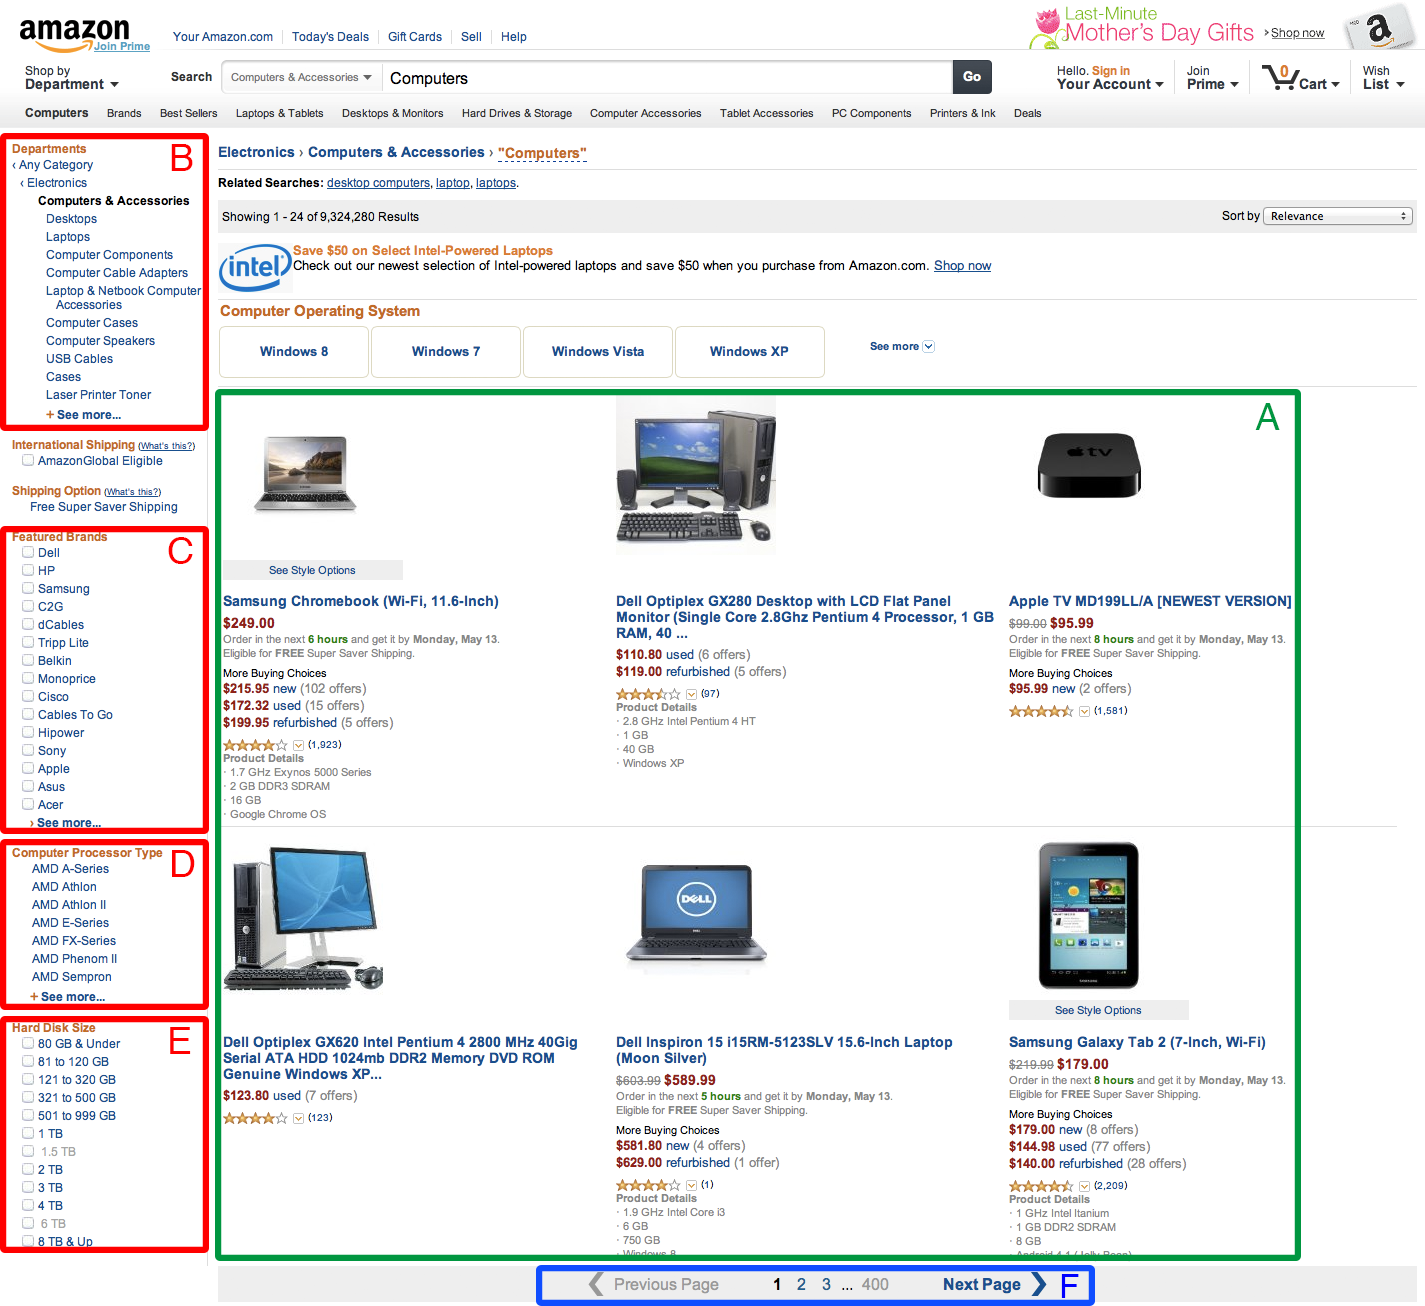
\includegraphics[scale=0.40]{imgs/chap_2/Amazon.png}
\caption{An example of Amazon Web page}
\label{fig:amazon1}
\end{figure}

Figure~\ref{fig:amazon1} shows an Amazon web page returned for the query \textit{Computer}. In such page it is possible identify several groups of structural data. In particular, links in structured data that describe the product listing (i.e., box A) allow us to obtain key information related to real-world entities (e.g., computers) while links contained in the other structured data (boxes B, C, D, E, F) allow us to navigate the organization of the website and identify meaningful connections among objects (e.g., identify computers belongs to the same brand).

Extracting such data records is useful in several application domains because it enables us to obtain and integrate data from multiple sources (websites and web pages) to provide value-added services, e.g., customizable web information gathering, comparative shopping, meta-search, etc. With more and more companies and organizations disseminating information on the Web, the ability to extract such data from
web pages is becoming increasingly important.

%Differently from traditional textual documents, structured data in web pages are enriched by hyperlinks that enable information to be splitted in multiple and interdependent web pages. These hyperlinks can be used to identify collections real-world entities (e.g., web pages of courses, professors, products, news, etc) and relationships among entities.  Figure~\ref{} shows an Amazon web page returned for the query \textit{Computer}. In such page it is possible identify several groups of structural data. In particular, links in structured data that describe the product listing allow us to obtain key information related to real-world entities (e.g., computers) while links contained in the other structured data allow us to navigate the organization of the website and identify meaningful connections among objects (e.g., identify computers belongs to the same brand). 

Although these data are easily identified by humans, machines are not able to directly access to structured data encoded in web pages. Moreover, since web documents are neither well structured such as database nor completely unstructured such as pure textual documents, traditional Data Mining or Text Mining techniques can not be directly applied on structured data encoded in web pages.

%In the first case, Data Mining techniques are based on the assumption that data used to learn models share a common schema and be independent among them. 
In the first case, Data Mining techniques are based on the assumption that data used for learning models share a common schema having well defined tables, attributes (columns), tuples (rows), keys, and constraints. Moreover, such data should be independent among them. 
Web pages break this assumption because structured data do not share a common schema and their hyperlinks define interdependence relationships among web records and web pages. Moreover, web pages are codified in HTML a markup language that, differently from other language markups used to store data such as XML, was projected just for data rendering. Consequently, the Web can be considered a modern legacy system because such a large body of data cannot be easily accessed and manipulated. 

In the second case, Text Mining techniques extract structured data in web pages analyzing recurrent patterns and named entities in word sequences~\cite{Sarawagi:2008}. Existing solutions for plain documents fail to learn accurate models because they are based on assumption that the document collection is written with a consistent writing style (e.g., news articles). Moreover, text mining approaches, considering documents as sequences of words, are not able to extract valuable information from different web page's representations. In fact, differently from textual documents, web pages have multiple representations which provide different information; one is the text representation written in HTML; the other is the visual representation rendered by a web browser. These sources of information are completely ignored by Text Mining approaches. As consequence, they are not able to handle complex information within web elements possessing various semantic roles (e.g., a navigation menu, main content, calendar, table, and logotype) and providing different functionalities (e.g., a link, button, and element with drag-and-drop function)~\cite{Qi:2009}. Finally differently from textual documents, web pages are enriched by hyperlinks that enable information to be splitted in multiple and interdependent web pages. These hyperlinks can be used to identify collections real-world entities (e.g., web pages of courses, professors, products, news, etc) and relationships among entities. Also this information is ignored by Text Mining. 

Consequently, there is a strong need in the computer science field of creating techniques and approaches that, using textual, structural, and visual information of web pages, are able to extract schema from structured data and align the data using that schema. 
Goal of Web Information Extraction is that to transform the Web from a legacy system to the biggest, structured, and easily accessible database. 

%\section{Structured Data in the Web}
%\label{sec:Structured Data in the Web}  
%\color{red}
%A large amount of information from the Web is represent in form of semi-structured data, that is a combination of unstructured text with data having a structure or a schema~\cite{Arasu:2002}. Structured data contained in web pages are typically \textbf{data records} generated dynamically from an underlying structured source like a relational database (e.g., product listing of an Amazon web page) or from a  static template (e.g., menus, navbars, etc.).

%Extracting such data records is useful in several application domains because it enables us to obtain and integrate data from multiple sources (websites and web pages) to provide value-added services, e.g., customizable web information gathering, comparative shopping, meta-search, etc. With more and more companies and organizations disseminating information on the Web, the ability to extract such data from web pages is becoming increasingly important.

%Differently from traditional textual documents, structured data in web pages are enriched by hyperlinks that enable information to be splitted in multiple and interdependent web pages.
%These hyperlinks can be used to identify collections real-world entities (e.g., web pages of courses, professors, products, news, etc) and relationships among entities. 
%Figure~\ref{} shows an Amazon web page returned for the query \textit{Computer}. In such page it is possible identify several groups of structural data. In particular, links in structured data that describe the product listing allow us to obtain key information related to real-world entities (e.g., computers) while links contained in the other structured data allow us to navigate the organization of the website and identify meaningful connections among objects (e.g., identify computers belongs to the same brand). 

%As mentioned above, since web documents are neither well structured such as database nor completely unstructured such as pure textual documents, traditional Data Mining or Text Mining techniques can not be directly applied on structured data encoded in web pages.
%In the first case, Data Mining techniques are based on the assumption that data used to learn models share a common schema and be independent among them. 
%In the first case, Data Mining techniques are based on the assumption that data used for learning models share a common schema having well defined tables, attributes (columns), tuples (rows), keys, and constraints. Moreover, such data should be independent among them. 
%Web pages break this assumption because they contain heterogeneous data and their hyperlinks define interdependence relationships. Moreover, web pages are codified in HTML a markup language that, differently from other language markups used to store data such as XML, was projected just for data rendering. From this reason, the Web can be considered a modern legacy system, since such a large body of data cannot be easily accessed and manipulated. 
%In the second case, Text Mining techniques fail to learn accurate models on web pages because they require collection of documents written with consistent styles (e.g., news articles) and are not able to handle complex information with elements possessing various semantic roles (e.g., a navigation menu, main content, calendar, table, and logotype) and providing different functionalities (e.g., a link, button, and element with drag-and-drop function)~\cite{Qi:2009}. 
%In fact, differently from textual documents, web documents have multiple representations which provide different information. One is the text representation written in HTML; the other is the visual representation rendered by a web browser. Text Mining algorithms focus on the text representation while ignore the visual information.   

%Consequently, there is a strong need in the computer science field of creating techniques and approaches that, using textual, structural, and visual information of web pages, are able to extract schema from structured data and align the data using that schema. 
%Then the goal of Web Information Extraction is that to transform the Web from a legacy system to the biggest, structured, and easily accessible database. 
\section{The role of Information Extraction}
\label{sec:The role of Information Extraction}
%\color{green} introduzione a IE, trovare strutture nascoste nelle pagine web (vedi anche abstract dakkar)
%    e.s. strutture nelle tabelle
%         strutture nelle liste\\
\color{red}
Information Extraction born originally as a natural language processing task used to extract relevant information both from structured text with tabular information and from free text such as news articles~\cite{Eikvil:1999}. Goal of Information Extraction is to identify patterns involving syntactic relationships between words or semantic classes of words. Extracted patterns can be used generate a relation of k-tuple (where k is the number of attributes in a record) or a complex object with hierarchically organized data~\cite{Chang:2006}.
An application example is to extract from a terrorist attack article key information about perpetrators, their affiliation, victims, location, etc \cite{Pio:2014}. 

With the growth of the Web researches tried to apply information extraction techniques on web pages. %As said in the previous section a web page is considered structured if each attribute in a data record can be correctly extract based on some uniform syntactic clue, such as delimiters, visual alignments, etc, while it is considered semi-structured if it is not possible extract directly a complete schema due data records with missing attributes, attributes with multiple values, attribute permutations, and exceptions. 
%Figure~\ref{fig:ebay} shows an example of semi-structured web page with several missing attributes in data records (e.g., item description, original price, etc.).  
%\begin{figure}[t!]
%\centering
%\includegraphics[scale=0.25]%{imgs/chap_1/ebay_semiStructuredSchema.png}
%\caption{An example of semi-structured web page}
%\label{fig:ebay}
%\end{figure}
As said in the previous section, web pages differ from textual documents for several aspects, such as absence grammatical structures, presence of hyperlinks, etc.
For this reason, traditional information extraction tools which use linguistic knowledge to extract key information are not suitable for web pages. For example, most of structured data in web pages are rendered using regular HTML tags patterns and information are splitted in interconnected web pages. For these web pages the analysis of regularity on their visual and structural representation and the analysis of the graph behind the website can be used for extracting structured data more accurately and efficiently than natural language processing methods. 

Information extraction systems on the Web require to solve five distinct problems:
\begin{itemize}
\item \textbf{Navigation problem}: finding target web pages, i.e., pages containing data to extract in a website following hyperlinks. Websites, especially data intensive websites, contain both target pages and navigational pages (i.e., web pages contain hyperlinks to target pages or to other navigational pages). A system for extracting structured data should explore web pages in a way to minimize the search space to target pages and as less navigation pages as possible.  
\item \textbf{Data extraction problem}: extracting relevant data records from web pages. Solutions to extract data records should analyze structural and visual properties of web elements to find recurrent patterns which describe data records.
\item \textbf{Schema synthesis problem}: generating schema behind extracted data- records. In this case  solutions are needed to extract and align attributes from data records. These solutions should be able to handle missing values, values embedded in plain text paragraphs, values hierarchically organized, etc.  
\item  \textbf{Data mapping}: aggregating data from several websites. This requires data be homogenized since different websites can follow different conventions for naming things, for expressing measured units (e.g. currency, weight of a product, etc.), etc.. Mapping discrete values (e.g. company names) into a standard format and transforms measured values in a common unit improves the quality of the extracted data. 
\item \textbf{Data integration}: merging data from separate web pages. Some websites, especially websites with a large amount of data (e.g. Ebay, Amazon, etc.), split structured data on multiple web pages for avoiding to overload a single page with too much information (e.g., splitting the products listing using the pagination list). Other times information about a single data record are splitted on multiple web pages (e.g., reviews of a product and  main information about the product self are stored on two different 
web pages). 
Large scale programs able to fetch tens of thousands of web pages per second are called \textit{crawler, spiders, web robots, or bots}.
\end{itemize}

To extract structured data from the Web, several types of wrappers have been created. A wrapper can be defined as a program that extracts structured data of a particular information source and translates them into a relational form~\cite{Kushmerick:1997}.
Existing wrappers can be categorized in three main groups:
\begin{itemize}
\item \textbf{Manual wrapper}: it involves the writing of ad hoc code. Human programmers identify syntactic patterns to extract structured data analyzing source codes (i.e. HTML code) of web pages and understanding their structure. Although this approach is simple, it suffers several disadvantages due Web features. The first drawback is due by heterogeneity and dimension of the Web; manual wrappers are not scalable %to a large number of websites 
because websites and web pages with different structures require different wrappers. Moreover, the Web is a dynamic environment where web pages are created, destroyed and modified; wrappers can not automatically adapt to these changes since they are based on a specified grammar and manual maintenance has high cost.  
\item \textbf{wrapper induction}: it consists in the automatic wrappers construction based on inductive learning methods. The first wrappers were created around 1995-1996. In this case,  supervised learning approaches are used to automatically generate rules which are then used to extract structured data from unseen web pages. Wrappers based on induction learning can be classified as \textit{zero-order} or \textit{first-order} depending on the inductive learning method used~\cite{Eikvil:1999}. Wrappers constructed using zero-order learning methods learn models in form of couples \textit{attribute-values}, that is, from database point of view as disconnected relations. Differently from zero-order wrappers, first-order wrappers are able to learn models in form of first-order predicates which describe relations and associations between these relations.   

The accuracy of learned rules, and consequently the accuracy of this type of wrappers, strongly depends both the number and the quality of examples (i.e. manually labeled pages and data records). Wrappers generated using supervised learning require a high cost for manual labeling of examples, for generating wrappers from websites with different structure, and for the maintenance in case changes in the websites structure.
\item \textbf{automatic extraction}: it consists in the automatic wrappers construction based on unsupervised learning. Differently from the previous approaches it is not required the manual labeling effort. This makes wrappers scalable to a large amount of websites and easily maintainable. Modern wrappers are based on this approach.
\end{itemize} 

\section{The role of information network analysis}
\color{green}
% Web as Heterogeneus Information Network
%\color{green}
%https://books.google.it/books?id=yqOeBQAAQBAJ&pg=PA7&lpg=PA7&dq=browse+search+navigate+paradigms+web&source=bl&ots=avDgal_C_I&sig=ZvEpsTbNffjgs0ug18M2KbvegaA&hl=it&sa=X&ved=0ahUKEwiy8uLw9rXJAhVIDSwKHWw_Dv8Q6AEIOTAD#v=onepage&q=browse%20search%20navigate%20paradigms%20web&f=false
\color{red}
    %Information networks are ubiquitous and form a critical component of modern information infrastructure. Most of data or informational objects, individual agents, groups, or components are interconnected or interact with each other, forming numerous, large, interconnected, and sophisticated networks.
%The Web can be considered the largest, complex, and unexplored information network. In fact, it contains billion of shared and public availabe documents related to a complete range of topics, from product to financial, public-record, scientific, hobby-related, and government.\\

Nowadays, most real phenomena can be represented as information networks, that is graphs where the nodes are real-world entities interconnected and interacting among them. 
Formally an information network can be defined as follow \cite{Sun:2012}:
\begin{definition}
\label{def:network}\textbf{Information Network:}
is defined as a directed graph $G = ( V , E )$ with an object type mapping function $\tau : V \rightarrow A$ and a link type mapping function $\phi : E \rightarrow R$, where each object $v \in V$ belongs to one particular object type $\tau (v) \in A$ , each link $e \in E$
belongs to a particular relation $\phi(e) \in R$ , and if two links belong to the same relation type, the two
links share the same starting object type as well as the ending object type. 
\end{definition}

\begin{figure}[h]
\centering
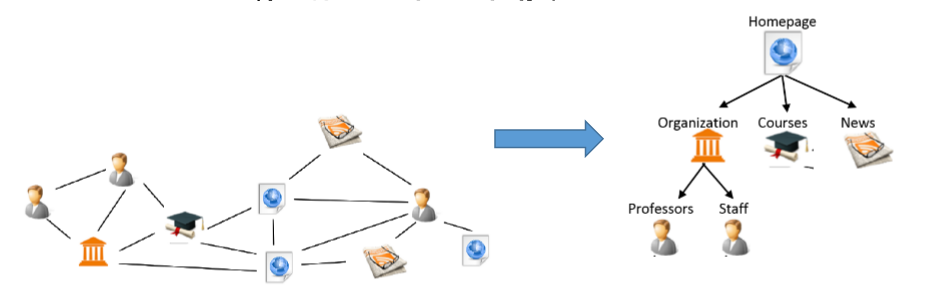
\includegraphics[scale=0.40]{imgs/chap_1/informationNetwork1.png}
\caption{An example of an information network of a website where nodes are web pages related to different entity types (e.g. people, news, organizations) and edges are hyperlinks}
\label{fig:informationNetw}
\end{figure}


The analysis of information networks %, or their special kinds, such as social networks \cite{Wasserman:1994} and the Web, 
has gained extremely wide attentions nowadays from researchers in several fields such as
computer science, social science, physics, economics, bioinformatics, and so on, with exciting discoveries and successful applications across all the disciplines. Goal of information network analysis is to extract patterns or regularities in relationships among interacting units which represent the structure of the network. 
For example, the application Data Mining or Graph Mining techniques on information networks allows researches to discover latent structures among nodes, such as the topics and communities they are involved in, the roles that different types of nodes play in these topics and communities, and the relations they potentially have with each other. These approaches can be used in the context of the Web for combining intra-page information (e.g. textual content, HTML structure) with inter-page information which describe the topological structure of websites.

Although several methods and approaches exist for extracting knowledge from the information networks, most of the existing studies are based on the assumption that  networks are homogeneous. %, that is nodes and relationships are of the same type. 
However, real information networks contain heterogeneous and structured data (e.g., relational database data) \cite{Sun:2012}. Although a single link in the network could be noisy, unreliable and sometimes misleading, valuable knowledge about the structure of networks can be discovered reliably analyzing massive connections between objects~\cite{Kargupta:2008}.
\section{Outline of the thesis}
%Vedere pagina 16 http://www0.cs.ucl.ac.uk/staff/J.Zhu/thesis.pdf

In this thesis I investigate the principles and methodologies for discovering novel and valuable knowledge from the Web.  I propose models and algorithms which exploit the main features of web pages and websites for extract structured information encoded in one or more web pages or hidden in the link structure of websites. Proposed methods involve several fields, ranging from Web Information Extraction to Information Network Analysis, Sequential Pattern Mining, Web Structure and Content Mining. Moreover, the methods and approaches analyzed and implemented in this thesis can contribute to give a structure to the Web exploiting and discovering properties and interactions among web pages that were previously unknow

%contibute to evaluate interactions among web pages, organize the content of websites and understand their structure. 

%and can contribute to give a structure to the Web and explore properties and interactions among web pages that were previously unknow. 

The major contributions are threefold. First, I propose a novel solution to extract structured data in form of \emph{web lists} splitted on multiple web pages. Although this task has been studied extensively, existing approaches are based on the assumption that lists are wholly contained in a web page. They do not consider that many websites span structured data of same semantic class (e.g. books, professors, product listing)  on several web pages and show for each of these only a partial view. Proposed method combine information intra-page (i.e web lists) and extra-page information (website structure) to extract a complete collection of structured data belonging to the same semantic class.

Second, a method to automatically discover sitemaps is realized. Actually  sitmaps are manually generated by web designer or automatically extracted by infomation network analysis tools. In the former, manual approaches extract static and deeper (with respect to automatic methods) hierarchies which are not able to capture evolutions in the website (e.g. generation of new sections, deletion of existing web pages, etc.). This makes sitemaps helpless and confusing for users after few time. In the latter, existing solution extract only a flat list of website's urls that do not show the hierarchical structure of a website or use only web pages' content ingnoring the website's link structure. Differently from existing automatic solutions, the proposed approach  is both automatic and effective. It explores navigation systems (e.g. menu, nav-bar, content list, etc.) contained in a website and exploits recurrent patterns of navigation systems to discover rich hierarchies that unveil relationships among web pages (e.g. relationships of super/sub category). For this scope, a novel sequential \emph{closed} pattern mining algorithm, called CloFAST, is implemented. CloFAST combines a new data representation of a sequence dataset  with a novel one-step technique to both generate sequences and to prune the search space. These features allows CloFAST to drastically reduce the number of
intermediate subsequences and then reduce the computational complexity of the sequence generation process while preserving the same
expressive power of patterns extracted by means of existing algorithms. Reducing the computational complexity of algorithms used the Web context is foundamental task.

Third, I focus on another challenging task in Web Mining: clustering of web pages. Web pages are characterized by different roles and several representations, based on textual, hyperlink and HTML formatting (i.e. HTML tags and visual) properties. Existing clustering algorithms use these information almost independently, mainly because it is difficult to combine them. Proposed solution is intended to be a contribution on clustering of web pages in a website by combining all this features into a single vector space representation. 






  

 




\chapter {Automatic Extraction of Logical Web Lists}
\label{chap:chap_1}
% !TEX encoding = UTF-8
% !TEX TS-program = pdflatex
% !TEX root = ./thesis.tex
% !TEX spellcheck = en

%************************************************

\section{Introduction}
The Web contains a large amount of structured data, most of which represent the main content of web pages. For example, given a Amazon web page that describes a DVD product, provided information about the item, such as prize, title, reviewers, ads, etc. are organized in a structured way. 

Although humans can easily understand how such information are structured (e.g., distinguish between the structured data and the rest of the web content),  machines cannot extract this semantic from
the HTML code.
Nowadays, to solve this issue two main approaches are applied: 
\begin{itemize}
\item Using data markups to encode machine-readable knowledge. These markups are not related to the formatting of data but they just make the metadata and text enclosed within the XHTML tags more meaningful to computers.   
\item Data Mining methods automatically extract structural data based on structural features, visual features or both. 
\end{itemize}
Although using data markups makes web pages machine-readable, there are several reasons why the first solution can not be applied on all websites. First, data intensive websites such as Deep Web Databases (e.g. Amazon.com, Trulia.com) are not favorable to make accessible all their information assets. Another important reason is that enriching web pages with XHTML tags requires human efforts which do not involve direct earnings for organizations' websites.\\
Several methods to extract structured data have been presented in the literature. The first approaches were hand-crafted web scrapers based on regular expressions. An obvious disadvantage of these approaches is that different rule expressions need to be manually created for each website. Furthermore, an individual website may also change its structure or layout over time
making this approach not scalable and in need of continuous maintenance. 
\\
Several supervised and unsupervised Data Mining methods were implemented later ~\cite{Liu2004,miao2009,Lerman2004,Gatterbauer2007,Liu2010}.
Although these methods close the challenge of automatic extraction of structured data from a web page, they fail to detect data record which span multiple web pages. \color{black}This is an open issue, because many websites, especially data-intensive (e.g. Amazon, Trulia, AbeBooks,\ldots), present their listings as \emph{logical list}, that is, a list spanning multiple pages (\textit{e.g.} computers, books, home listings)\footnote{The motivations behind this approach are as well technical (reducing bandwidth and latency), and non technical as avoiding information overload or maximizing page views.}. It is as if, each list represents a \emph{view} of the same \emph{logical list}. Similar to databases, where a \emph{view} can represent a subset of the data contained in a table partitioned over a set of attributes, a \emph{logical list} is split in multiple \emph{views} (web pages) in order to avoid information overload and to facilitate users' navigation. 

\begin{figure}[t!]
\centering
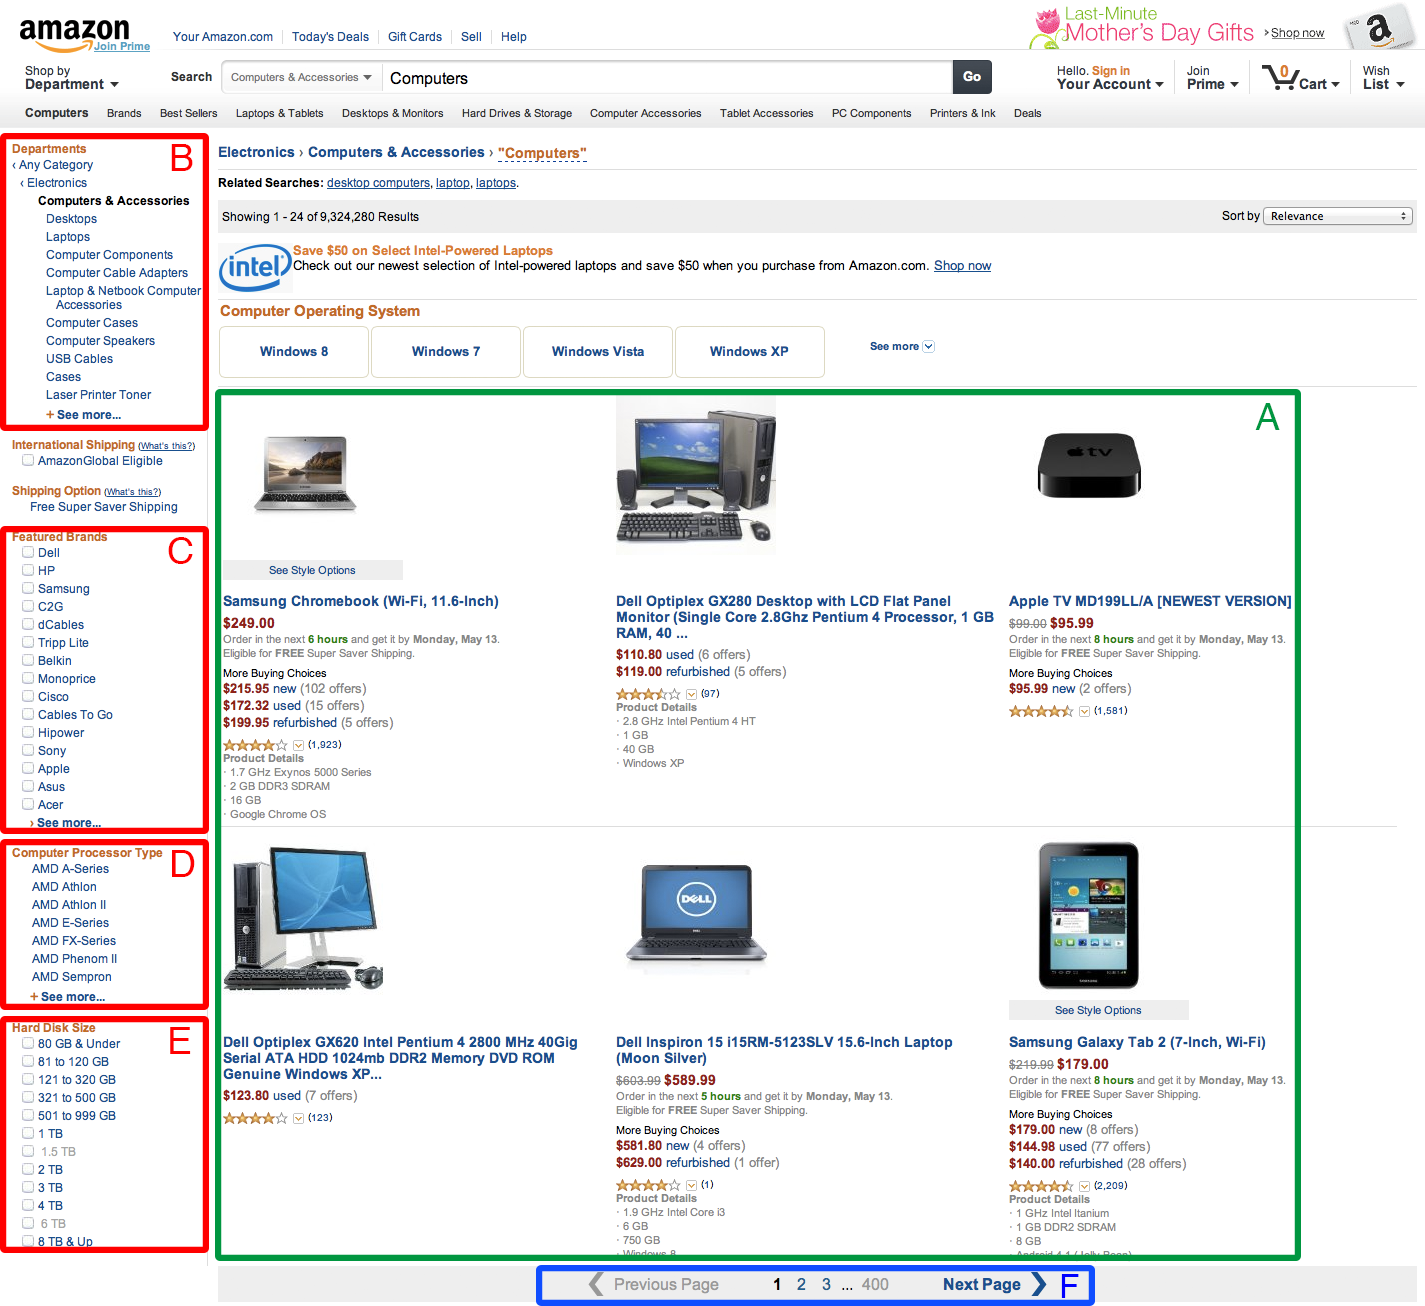
\includegraphics[scale=0.40]{imgs/chap_2/Amazon.png}
\caption{An example of Amazon web page}
\label{fig:amazon}
\end{figure}
For example, Fig.~\ref{fig:amazon} shows a web page from Amazon.com that contains the results for the query ``Computer''.
On this page, the boxes A, B, C, D, E, F are web lists. The list in the box A shows a \emph{view} of the ``Computers'' products, that is the top six sorted by relevance, and F allows us to navigate to the other views of the products ordered by relevance. Thus navigating the links in F we can generate the \emph{logical list} of the products for the query ``Computer''. Boxes B, C, D and E contain respectively the lists representing filters for ``Department'', ``Featured Brands'', ``Computer Processor Type'', and ``Hard Disk Size'', which are attributes of the \emph{virtual} table ``Computer''. Moreover, the anchor-text links in boxes B, C, D and E stores valuable information which can be used to annotate data records, and thus to individuate new attributes. For example, the anchor-text links of web list C can be used to index data records based on ``Computer brands''. Traditionally, search engines use the proximity of terms on a page as a signal of relatedness; in this case the computer brand terms are highly related to some data records, even though they are distant.

Providing automated techniques for \emph{logical list} extraction would be a significant advantage for data extraction and indexing services. Existing data record extraction methods~\cite{Liu2004,miao2009,Gatterbauer2007,Liu2010} focus only in extracting \textit{view} lists, while several commercial solutions\footnote{Lixto, Screen Scraper Studio, Mozenda Screen Scaper} provide hand-coded rules to extract \emph{logical lists}. 

In this chapter, I face this issue by proposing a novel unsupervised algorithm for automatic discovery and extraction of \emph{logical lists} from the Web. This method requires only one page containing a \emph{view list}, and it is able to automatically extract the \emph{logical list} containing the example \emph{view list}. Moreover, during the process, it enriches the list's elements with the pair \emph{$<$url, anchor-text$>$}  used for the extraction task. We have validated our method on a several real websites, obtaining high effectiveness.
\section{Definitions and Problem Formulation}
\label{2Definition}
In this section, I introduce a set of definitions that will be used through the thesis.

A web page is characterized by multiple representations, such as a textual representation (composed by web page terms), a visual representation (composed by information about rendered web page) and a structural representation (composed by HTML tags). For extracting logical lists both the visual and the structural representations are exploited. %For this reason, I provide in the following formal definitions which identify the sources of information exploited by the proposed method.

\begin{definition}
\label{def_chap2:structuralRepresentation}
A web page is characterized by a \textbf{Structural Representation} composed by web elements inscribed in HTML tags and organized in a tree-based structure. HTML tags can be applied to pieces of text, hyperlinks and multimedia data to give them different meaning and rendering in the web page.
\end{definition}
%Although a web page has a structural representation which distinguishes it from a plain and unstructured textual document, a web page can not be considered well structured such as a database because HTML is a language markup projected just for data rendering rather than for storing data such as XML.
 
\begin{definition}
\label{def_chap2:webLayout} The \textbf{ Web Page Rendering} is the process of laying out a spatial position of all the text/images and other web elements in a web page to be rendered.
\end{definition}


 
\begin{definition}
\label{def_chap2:visualRepresentation}
\textbf{Web Page Visual representation.} When a web page is rendered in a web browser (see Def.~\ref{def_chap2:webLayout}), the CSS2 visual formatting model~\cite{WiumLie99} represents the web page's elements by rectangular boxes that are laid out one after the other or nested inside each other by forming a tree, called \textbf{Rendered Box Tree}. By associating the web page with a coordinate system whose origin is at the top-left corner, the spatial position of each web page's element is fully determined by the tuple $(x,y,h,w)$, where $(x, y)$ are the coordinates of the top-left corner of its corresponding box (i.e. the position of the box in the rendered page), and $(h, w)$ are the box's height and width respectively (i.e. the size of the box in the rendered page). Therefore, the \textbf{Visual Representation} of a web page is given by its Rendered Box Tree.
\end{definition}

The rendered box tree can be generated by any web browser which follows W3C specifications for rendering~\cite{WiumLie99}. Moreover, the rendered box tree could have a completely different structure from that of the corresponding HTML tag tree. This because \emph{i) }a web page can be enriched of invisible elements (like the $<$head$>$ tag or elements that have \emph{display:none;} set), and \emph{ii}) the generation of the rendered box tree requires the execution of javascript and css code.
  
 \begin{figure*}
 \center
\subfloat[Box Structure]{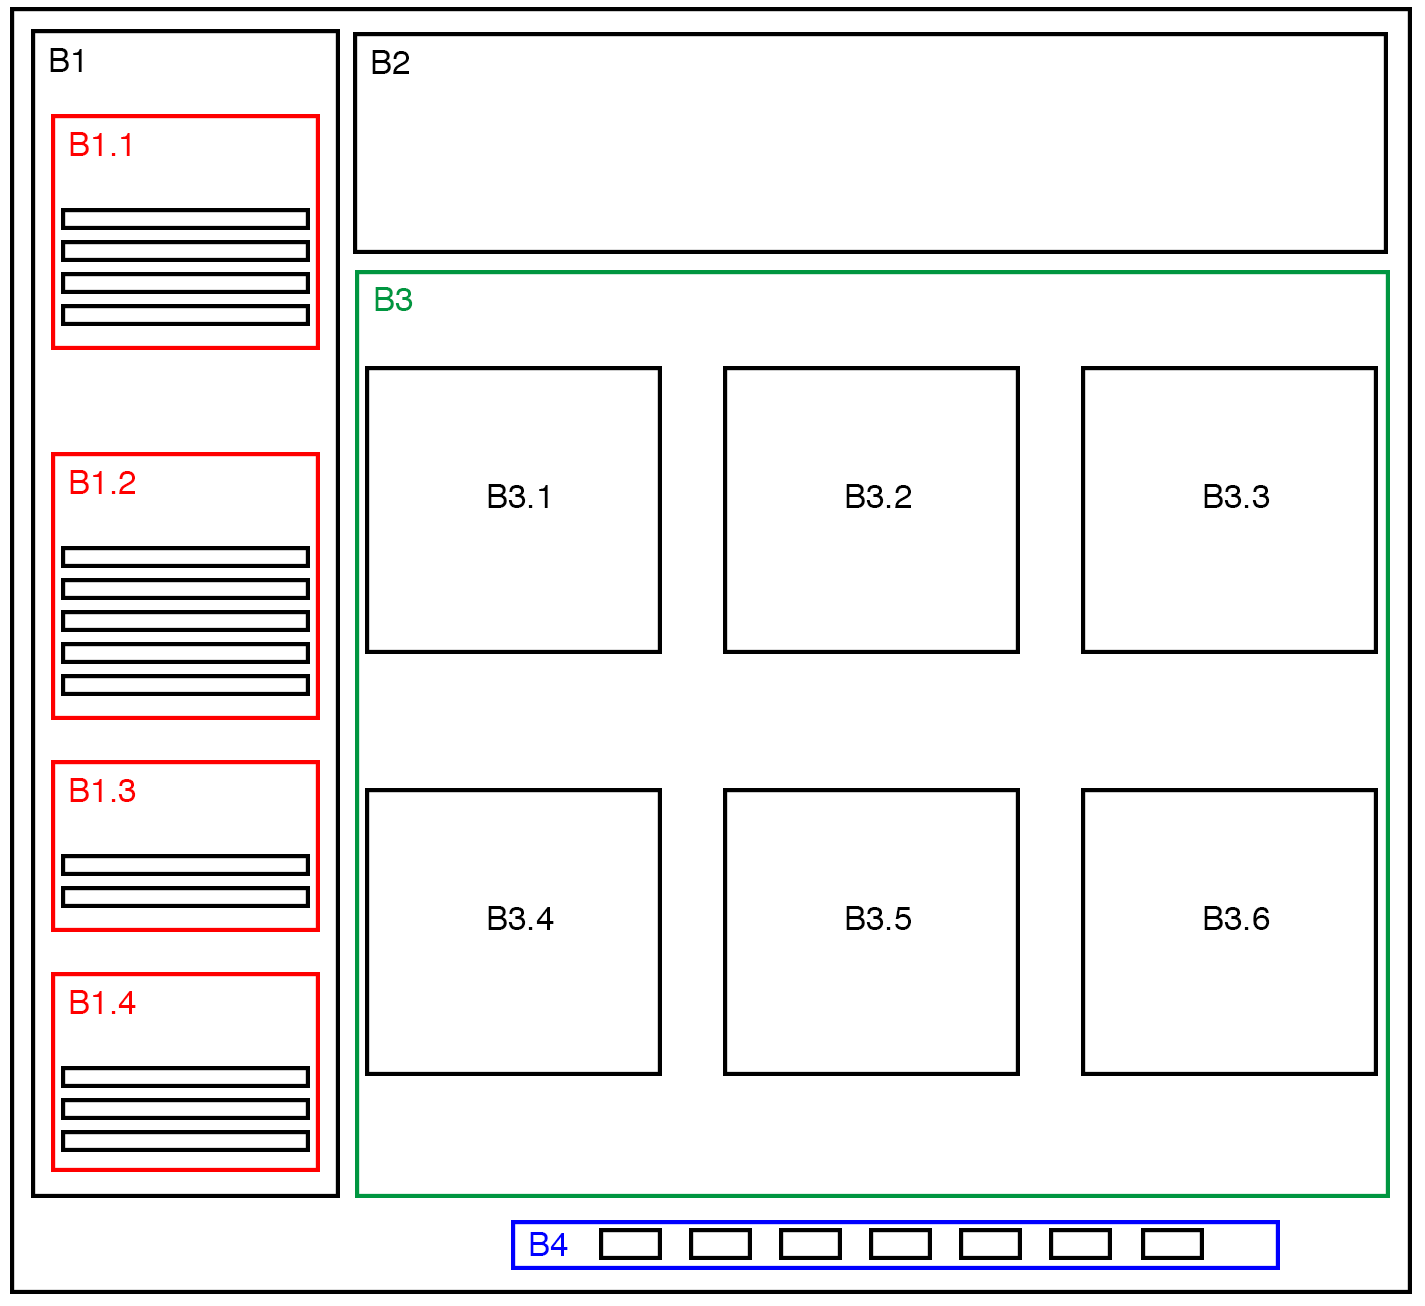
\includegraphics[scale=0.25]{imgs/chap_2/Rendered-box-tree1.png}} 
\subfloat[Rendered Box Tree]{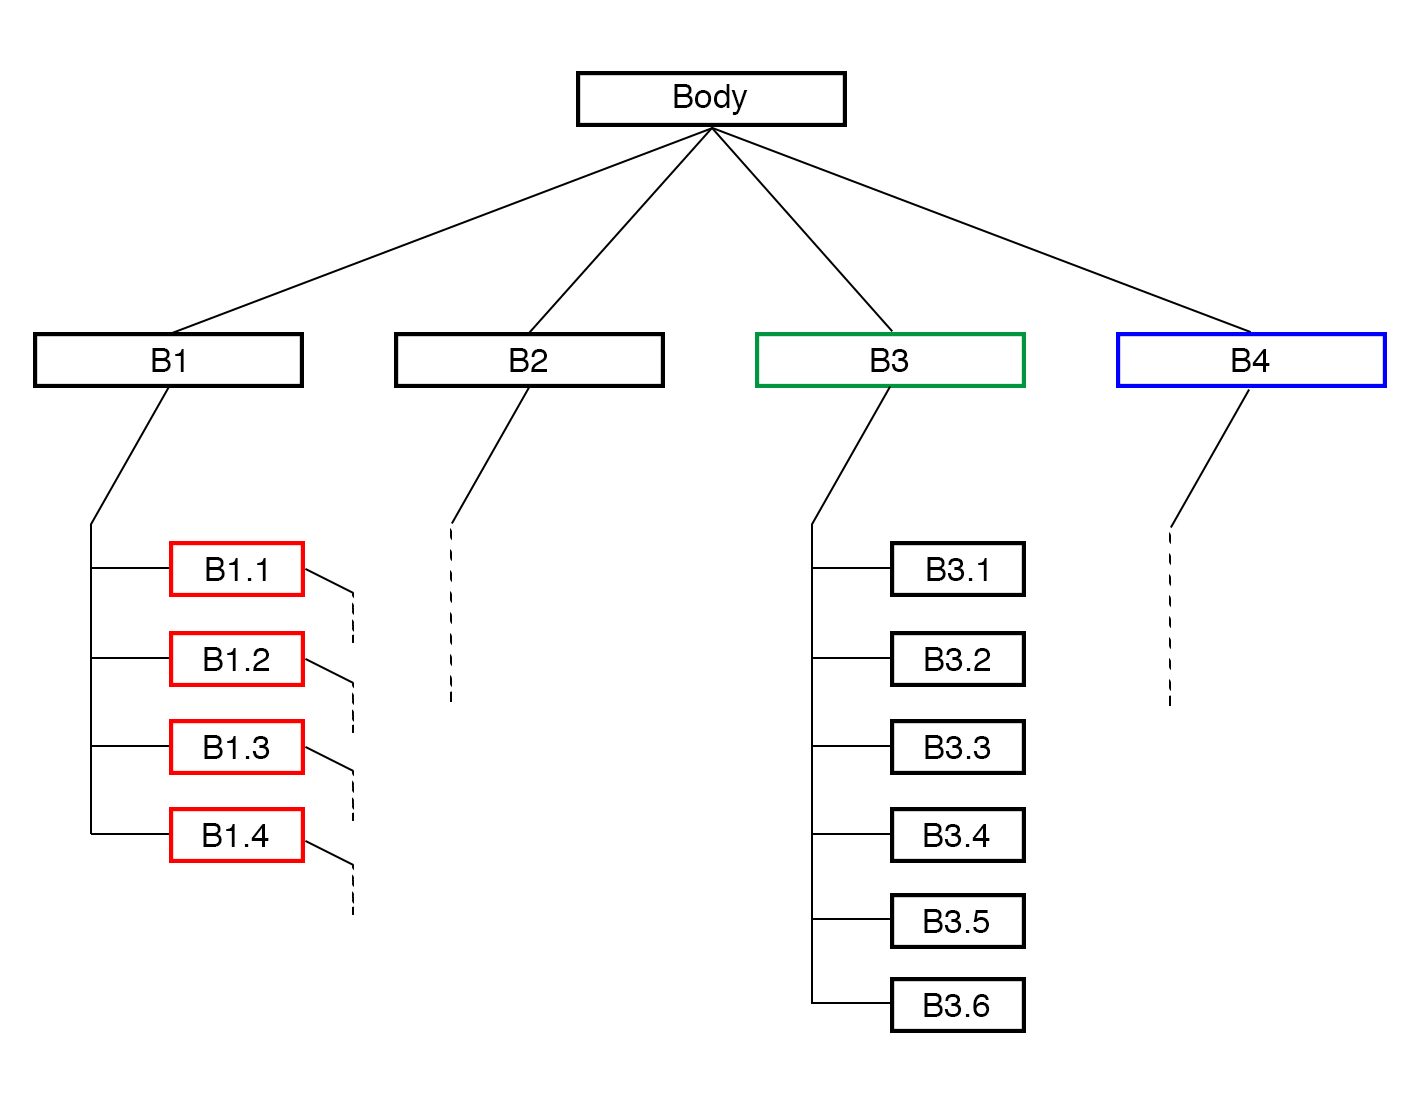
\includegraphics[scale=0.30]{imgs/chap_2/Rendered-box-tree2.png}}\
\subfloat[Structural Representation]{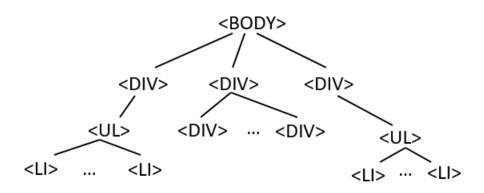
\includegraphics[width=2.5in]{imgs/chap_3/html}} 

\caption{}
\label{fig:Amazon2}
\end{figure*}

 
Figure~\ref{fig:Amazon2} shows an example of the structural and visual representations for the Amazon web page in Fig.~\ref{fig:amazon}. Leafs of the structural tree and the Rendered Block Tree represent the minimum semantic units that cannot be segmented further (e.g., images, plain texts, links).
Actually, the Rendered Block Tree is more complicated than what Figure~\ref{fig:Amazon2}(b) shows (there are often hundreds or even thousands of blocks in a Rendered Block Tree). 


Both Definition \ref{def_chap2:structuralRepresentation} and Definition \ref{def_chap2:visualRepresentation}, which are used to exploit the web page stucture, are used in the definition of web lists, which is crucial for the task of logical list extraction:

\begin{definition}
\label{def_chap2:list}
A \textbf{Web List} is a collection of two or more web elements (called data records) codified as rendered boxes having a similar HTML structure, and visually adjacent and aligned. This alignment can occur via the x-axis (i.e. a vertical list), the y-axis (i.e. horizontal list), or in a tiled manner (i.e. aligned vertically and horizontally)~\cite{Lanotte:2014}. 
\end{definition}

This definition requires an algorithm which is charge of checking whether two rendered boxes ``have a similar HTML structure''. Moreover, it also requires a formal definition of alignment and adjacency. These aspects are discussed in Section \ref{SecChap2:Methodology}.

From the Amazon web page, showed in Fig.~\ref{fig:amazon} it is possible to extract one tiled list (i.e., box A), one horizontal list (i.e., box F) and four vertical lists (i.e., boxed B, C, D, E). 

\begin{definition}
A \textbf{Data Record} identifies an element of a web list. Similar to the concept of data records into database, data records into a web page are a set of similar and structured objects containing information related to a real-world entity. 
\end{definition}

\begin{definition}
\label{def:logicalList}\textbf{Logical List}:
It is a list whose Data Records are distributed on more then one web pages. 
\end{definition}
An example is shown in Fig.~\ref{fig:amazonDiscovery}, where the boxes A1 and A2 represent a part of a \emph{logical list}.
\begin{definition}
\label{def:viewList}\textbf{View List}:
It is a view of a logical list, whose Data Records are all contained in same web page.
\end{definition}
List F in Fig.~\ref{fig:amazon} is an example of a view list. In fact, it contains only some of data records belonging to its logical list (that is the \textit{pagination list}).
\begin{definition}
\label{def:domList}\textbf{Dominant List:} It is the view list of interest, containing data records from the logical list that we want to extract.
%\textbf{Dominant List:} It is the view list of interest, containing the logical list's data records that we want to extract.
\end{definition}
%The list F in Fig.~\ref{fig:amazon} is an example of a view list. In fact it contains only some of data records belonging to its logical list (that is the \textit{pagination list}).
The choose of the dominant list strictly depends on the application goals. For example, if we want extract the whole product listing in an e-commerce website returned by a query, the dominant list is the web list containing products self (i.e. box A in Fig.~\ref{fig:amazon}). However, we could be interested to the navigation systems of a web page. In that case our dominant list could be for example its pagination list (i.e., box F in Fig.~\ref{fig:amazon}).  

%For example the list A in Fig.~\ref{fig:amazon} is the Dominant List for the given Web page.
%Finally in Figure~\ref{fig:amazonDiscovery}, where the boxes A1 and A2 represent a part of a \emph{logical list}.

\section{Methodology}
\label{SecChap2:Methodology}
In this section, I describe the methodology used for \emph{logical list} extraction process. The algorithm employs a three-step strategy.
Let $P$ a web page, it first extracts the set $L^P$ of the lists contained in $P$; in the second step, it identifies the \textit{dominant list} $l_{dom}^P \in L$; finally, it uses $l_{dom}^P$ to discover the \emph{logical list} $LL$ which includes $l_{dom}^P$ as sub-list. 
These steps are detailed in the following sub-sections.

\begin{figure}
\centering
	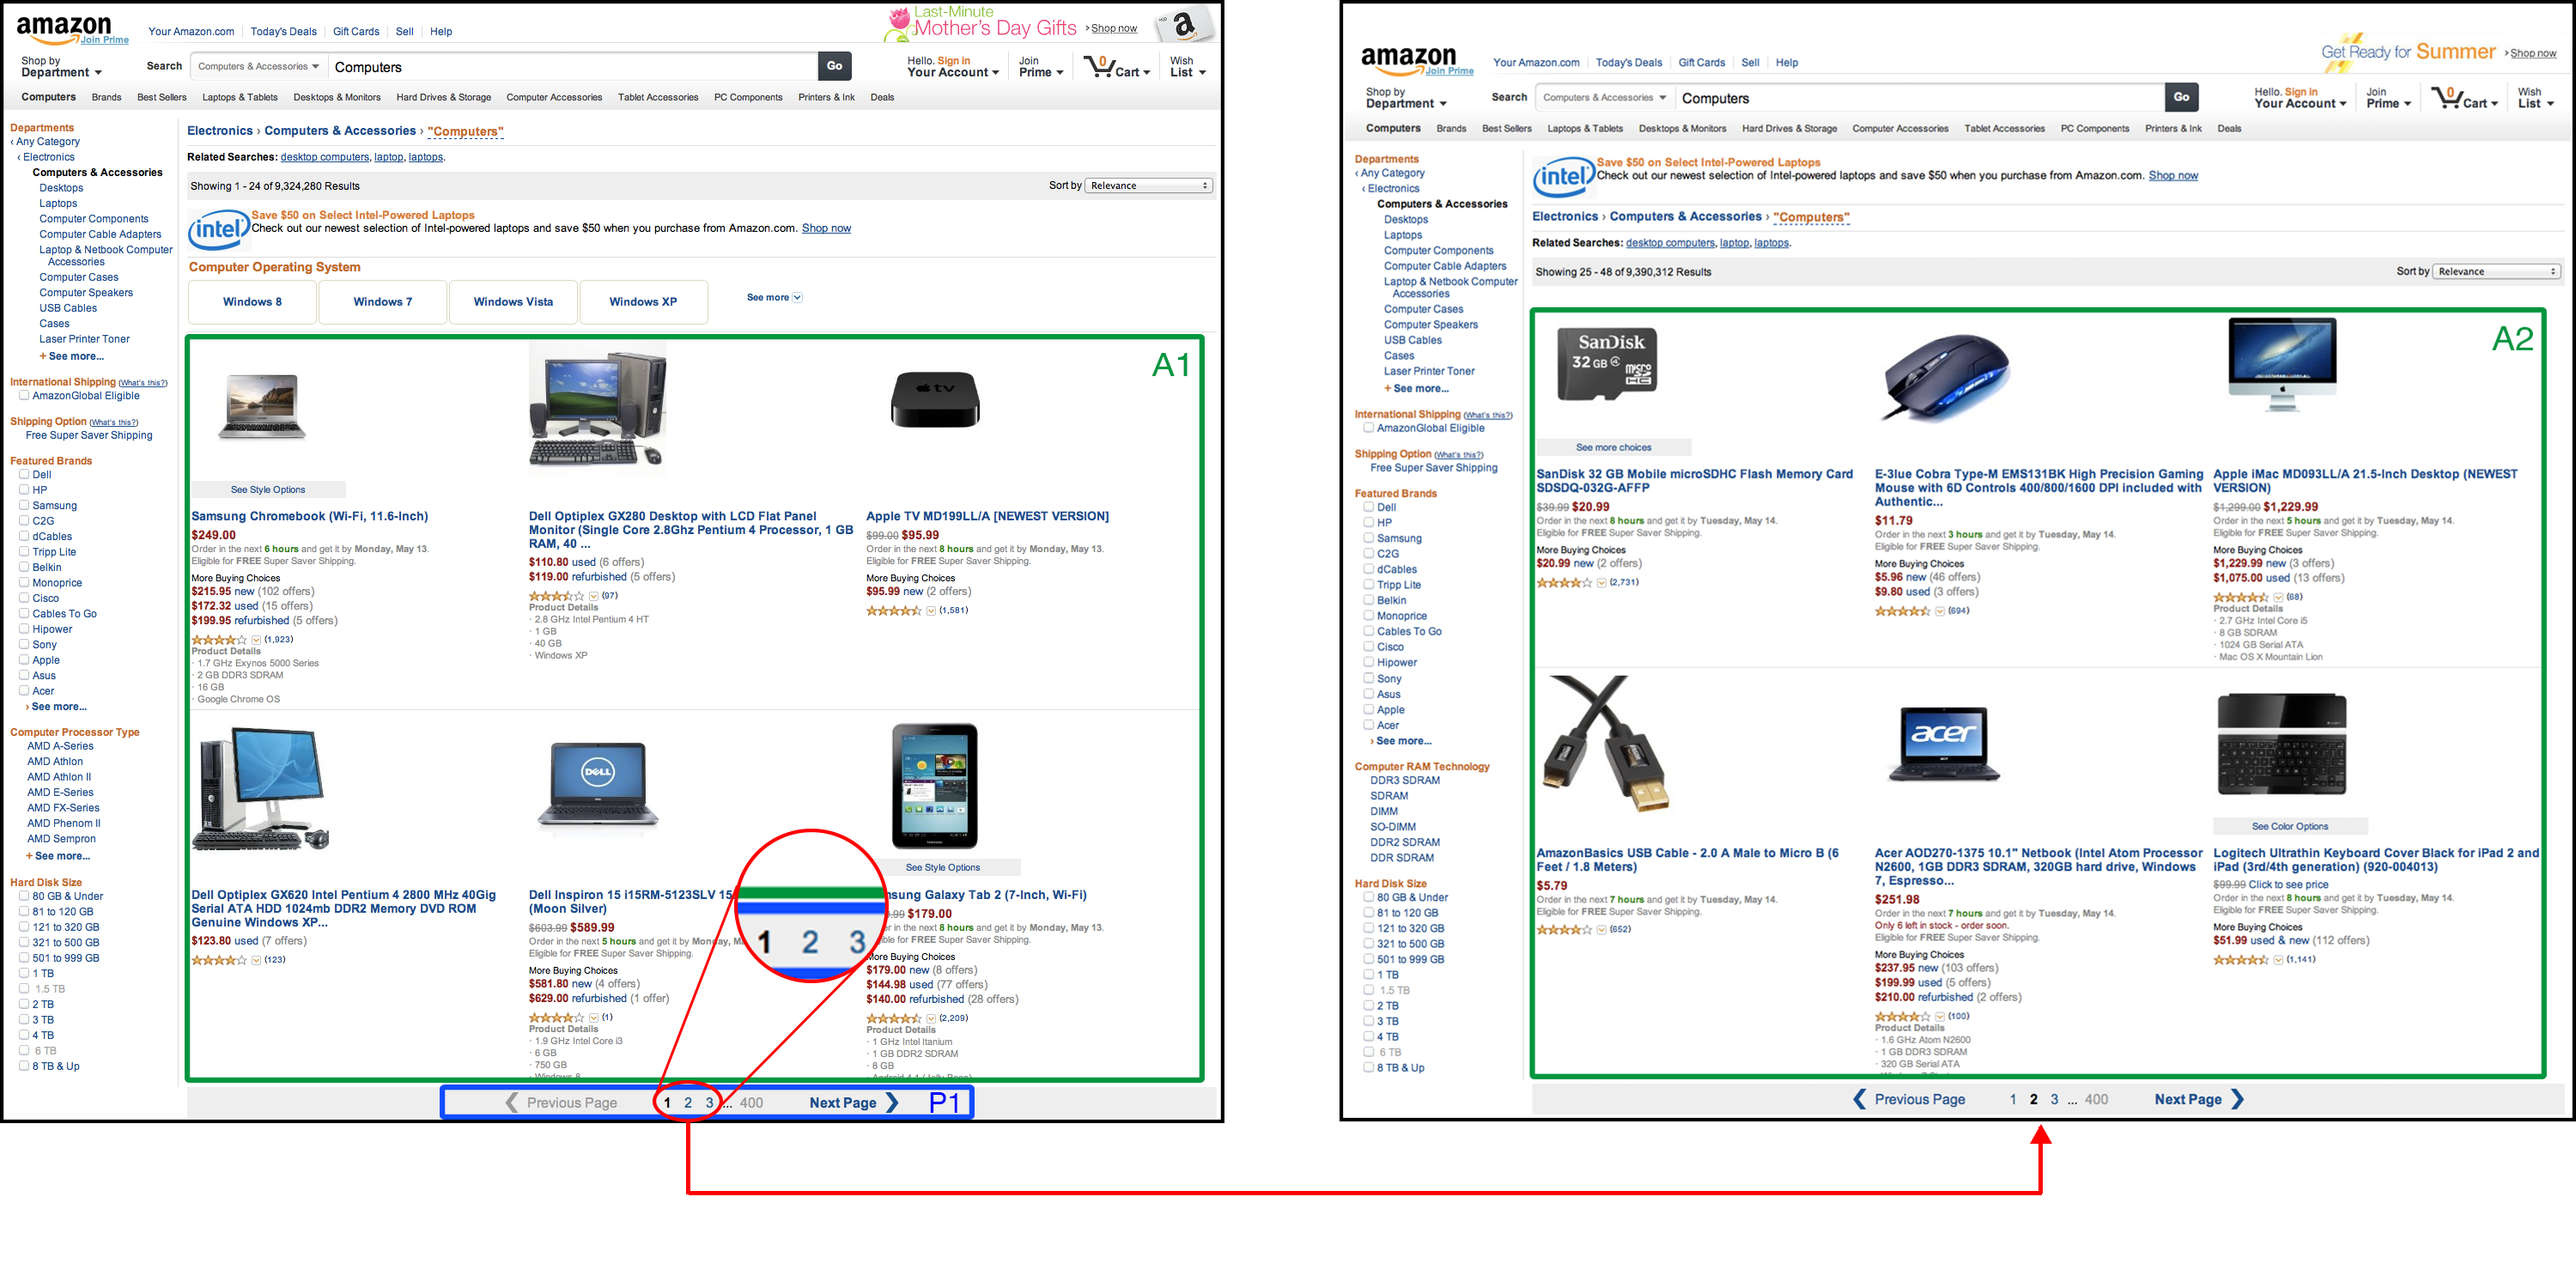
\includegraphics[scale=0.2]{imgs/chap_2/Amazon-discovery.png}
\caption{An example of \emph{logical list} for Amazon's products.}
\label{fig:amazonDiscovery}
\end{figure}

\subsection{List Extraction}
\label{2ListExtraction}
Given a web page $P$ as input, its web lists $L=\{l_1,l_2,\ldots,l_n\}$ are extracted. 
According to Definition \ref{def_chap2:list}, Algorithm \ref{chap2alg:extractWebLists} describes in detail the process of web list extraction. Before to analyze the implementative aspects of this algorithm we need to explore the concepts of \emph{structural similarity}, \emph{adjacency} and \emph{alignment}, between web elements, mentioned in Def.~\ref{def_chap2:list}. 

To check whether two web elements $e_i, e_j$ have similar HTML structure several distance measures can be applied. In the following we describe the measures used, throw this thesis, for computing the structural similarity among web elements:
\begin{itemize}
\item \textit{Normalized Edit Distance}. 
It measures the difference between two strings (or sequences) in terms of the minimum cost needed to transform a string $A$ into the string $B$ (through inserting, deleting or updating operations). This measure is then normalized for the maximum strings' length.
\begin{equation}
NormalizedEditDistance(A,B) = \frac{EditDistance(A,B)}{max(|A|,|B|)}
\end{equation}
For a survey on the Normalized Edit Distance and its variances see~\cite{Yujian:2007}.
For applying the normalized edit distance to two HTML tag trees (web elements) $e_i, e_j$, a conversion step to translate each HTML tag tree into a string format is required. For this scope, each HTML tag in the tree rooted at $e_i$($e_j$) is first codified into a unique character. Then, a string is extracted from the converted tree by applying a breadth search on its nodes. Figure~\ref{fig:NormalizedEditDistance} shows an example of an HTML tag tree rooted at tag $<body>$ and its converted tree. Applying a breadth search to the converted tree, we obtain the string $abbbcbbcdddd$.
Normalized edit distance is suitable to extract web lists whose data records have a simple and a very similar HTML structure (such as most web lists describing websites' navigation systems). To discover more complex web lists, in terms of structural representation, the normalized edit distance can be replaced by the \emph{Normalized Tree Edit Distance}
\item \textit{Normalized Tree Edit Distance.} Similar to the edit distance between strings, the tree edit distance between two trees $A$ and $B$ is the cost associated with the minimum set of operations needed to transform $A$ into $B$. 
Although tree edit distance algorithms are in general computationally more expensive than string edit distance algorithms, they are more accurate to extract web lists whose data records have deep and complex structural representations. %Therefore, if we want extract the product web list of a web page (e.g. box A in Fig.~\ref{fig:amazon}) the Normalized Tree Edit Distance should returns more accurate results than normalized edit distance.
For a survey on the Normalized Tree Edit Distance and its variances see~\cite{Demaine:2009}. For the scope of this thesis I have implemented the Tree Edit Distance proposed in \cite{Zhai:2005} and I have normalized it with the maximum number of nodes contained in $A$ or $B$.
\begin{equation}
NormalizedTreeEditDistance(A,B) = \frac{TreeEditDistance(A,B)}{max(|A|,|B|)}
\end{equation}
\end{itemize}

\begin{figure*}
 \center
\subfloat[Example of an HTML tag tree]{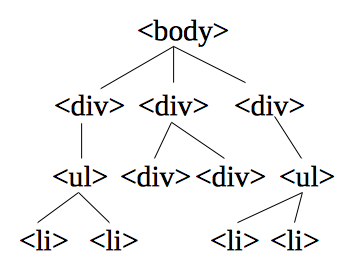
\includegraphics[scale=0.50]{imgs/chap_2/htmlTree.png}} 
\subfloat[Example of a converted HTML tag tree]{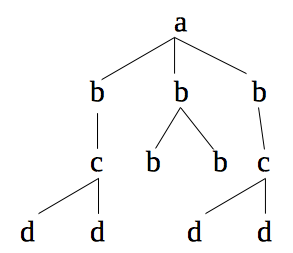
\includegraphics[scale=0.50]{imgs/chap_2/convertedTree.png}}
\caption{}
\label{fig:NormalizedEditDistance}
\end{figure*}
In addition to the structural similarity, other concepts required for the task of web list extraction are those of adjacency and alignment. 
In particular, two web elements $e_i, e_j$ are adjacent if they are siblings in the Rendered Box Tree and there is no  web element $e_w$, with $e_w \neq e_i \neq e_j$, which is rendered between them. Finally, two web elements $e_i, e_j$ are aligned on: \emph{i)} the x-axis if the have same $x$ coordinate, that is $e_i.x = e_j.x$; \emph{ii)} the y-axis if they share the same $y$ value, that is $e_i.y = e_j.y$; \emph{iii)}  both axes, that is $e_i.x = e_j.x$ and $e_i.y = e_j.y$.

After having defined the concepts of structural similarity, adjacency and alignment,  we can describe the method \emph{extractWebLists()} (Algorithm~\ref{alg:extractWebLists}). In particular, the algorithm starts analyzing all the nodes which, in the rendered box tree, are children of the rectangular box representing the \emph{body tag} element (line 2). For each node to analyze (line 4), only if the number of nodes in the subtree rooted in that node is relatively small, the algorithm tries to align its children (lines 9-30). Otherwise, it only enqueues the children for further processing. The rationale is that only small subtrees of the rendered box tree can represent weblists, whereas  subtrees rooted at the higher levels of the rendered box tree typically do not represent any structured data. For the experiments, the threshold value we use for the size of the tree (\emph{maxSize}) is 60. 
Only the nodes which are included neither in \emph{verticalLists} (which contains vertically aligned web elements) nor in \emph{horizontalLists} (which contains horizontally aligned web elements) are further explored by the algorithm (lines 27-28). 
The method \textit{getStructurallySimilar()} is the method that checks whether the elements in a list have similar HTML structure. In this chapter the normalized tree edit distance is applied.

\begin{algorithm}[H]
\caption{extractWebLists(P)}
\label{chap2alg:extractWebLists}
\begin{algorithmic}[1]
\renewcommand{\algorithmicrequire}{\textbf{Input:}}
\renewcommand{\algorithmicensure}{\textbf{Output:}}
\newcommand{\RETURN}[1]{\textbf{return} #1}
\renewcommand{\algorithmiccomment}[1]{$//$ \textit{#1}}
\renewcommand{\algorithmicforall}{\textbf{for each}}
\newcommand{\extractWebLists}[1]{ \textit{extractWebLists}(#1); }
\newcommand{\getChildren}[1]{ \textit{getChildren}(#1);}
\newcommand{\findElementByTagName}[1]{ \textit{findElementByTagName}(#1);}
\newcommand{\dequeue}[1]{ \textit{dequeue}(#1); }
\newcommand{\getVerticallyAligned}[1]{ \textit{getVerticallyAligned}(#1);}
\newcommand{\getHorizontallyAligned}[1]{ \textit{getHorizontallyAligned}(#1);}
\newcommand{\getStructurallySimilar}[1]{ \textit{getStructurallySimilar}(#1)}
\newcommand{\getNotAligned}[1]{ \textit{getNotAligned}(#1);}
\newcommand{\add}[1]{ \textit{add}(#1); }
\newcommand{\enqueue}[1]{ \textit{enqueue}(#1); }
\newcommand{\getUrls}[1]{ \textit{getUrls}(#1) }
%\SetKwFunction{FMain}{Main}
\REQUIRE web page P;
\ENSURE List$<$List$<$Web elements$>>$ L; //list of weblists.
\STATE body = webpage.\findElementByTagName{''body''}
\STATE notAligned = body.\getChildren{}
\REPEAT 
	
	\STATE node = notAligned.\dequeue{}
	\STATE children = node.\getChildren{}
	
	\IF{ node.getSize() $>=$ maxSize}
	\STATE notAligned.\enqueue{children}
	\ELSE 
	%\STATE verticalLists = children.groupBy(c $\rightarrow$ c.x)
	%\\.map(list $\rightarrow$ \getStructurallySimilar{list}) 
	%\\.filter(list $\rightarrow$ list.size $\geq$ 2)
    \STATE verticalAligned= children.groupByX();
    \STATE horizontalAligned = children.groupByY();
    
    \FORALL{list $\in$ verticalAligned}
    \STATE structurallySimilar = getStructurallySimilar(list);
    \IF{ structurallySimilar.getSize() $\geq$ 2}
    \STATE L.add(structurallySimilar);
    \ENDIF
	\ENDFOR 
	
	\FORALL{list $\in$ horizontalAligned}
    \STATE structurallySimilar = getStructurallySimilar(list);
    \IF{ structurallySimilar.getSize() $\geq$ 2}
    \STATE L.add(structurallySimilar);
    \ENDIF
	\ENDFOR 
	
	\STATE notIncluded = children - lists.getWebElements();
	\STATE notAligned.\enqueue{notIncluded}
	\ENDIF


\UNTIL{!notAligned.empty()}
\RETURN{L}


\end{algorithmic}
\end{algorithm}

\subsection{Dominant List Identification}

Given a web page $P$ and the set of list $L=\{l_1,l_2,\ldots,l_n\}$ extracted in the first step, three measures are used to identify the \textit{dominant list} of P: 
\begin{itemize}
\item \textbf{Centrality.} Given a list $l_i \in L$, the \emph{centrality} of $l_i$ w.r.t P is obtained by computing the Euclidean distance between the center of the parent-box of $l_i$ and the center of root-box of $P$.
\item \textbf{Area Ratio.} Given a list $l_i \in L$, the \emph{area ratio} of $l_i$ w.r.t P is the size of the box containing $l_i$ divided the size of root-box of $P$.
\item \textbf{Text-Tag Ratio.}  Given a list $l_i \in L$, and let $m$ the length of $l_i$, the \emph{text-tag ratio} of $l_i$ is computed as:
\begin{equation}
 \frac{1}{m}\sum_{j=0}^m \frac{chars(l_i[j])}{tag(l_i[j])}
\end{equation}
where $tag(l_i[j])$ is the number of HTML tags contained in the j-th data record of $l_i$ and $chars(l_i[j])$ is the total number of characters contained in $l_i[j]$. 
Before that the text-tag ratio is computed, \textit{script} and \textit{remark} tags
are removed because this information should be not considered in the count of non-tag text. 
\end{itemize}
In particular the \textit{Dominant list} of P is the list with  the highest sum of contributions:
\begin{equation}
\argmax_{{l_i \in L}} \frac{\alpha_1}{centrality(l_i)} + \alpha_2areaRatio(l_i)+ \alpha_3textTagRatio(l_i)
\end{equation}
where $centrality(l_i), areaRatio(l_i)$ and $textTagRatio(l_i)$ are respectively the centrality measure, area ratio and text-tag ratio of a list $l_i$ contained in L. $\alpha_1=\alpha_2=\alpha_3$ are set to $0.3$ to give the same weight to each measure.

%\begin{algorithm}
%\caption{\texttt{LogicalListDiscovery}}\label{alg:lld}
%
%\begin{algorithmic}[1]
%%\SetKwInOut{Input}{input}
%%\SetKwInOut{Output}{output}
%\renewcommand{\algorithmicrequire}{\textbf{Input:}}
%\renewcommand{\algorithmicensure}{\textbf{Output:}}
%\REQUIRE{ dominant list $l_{dom}^P$, set $L_{-}=\{L \setminus l_{dom}^P\}$}
%\ENSURE{ logical list $LL$}
%%\Input{ dominant list $l_{dom}^P$, set $L_{-}=\{L \setminus l_{dom}^P\}$}
%%\Output{ logical list $LL$}
%%\BlankLine
%		\STATE $LL = \{l_{dom}^P\}$%\;
%		\FORALL{$l \in L_{-}$}
%			\FORALL{$u \in l$}
%				$L_u \gets$ HyLiEn$(u)$%\;
%				$L_u$.filterSimilarity($l_{dom}^P,\alpha$)%\;
%				$LL$.add($L_u$)%\;
%	  \STATE $LL \gets LL$.flatMap()%\;
%	  \STATE $LL \gets LL$.removeDuplicates()\;
%	  \RETURN {$LL$}%\;
%\end{algorithmic}
%\end{algorithm}

\begin{algorithm}
\caption{\texttt{LogicalListDiscovery}}\label{alg:lld}

\begin{algorithmic}[1]
%\SetKwInOut{Input}{input}
%\SetKwInOut{Output}{output}
\renewcommand{\algorithmicrequire}{\textbf{Input:}}
\renewcommand{\algorithmicensure}{\textbf{Output:}}

\REQUIRE dominant list $l_{dom}^P$, set $L_{-}=\{L \setminus l_{dom}^P\}$
\ENSURE logical list $LL$
\STATE $LL = \{l_{dom}^P\}$
\FORALL{$l \in L_{-}$}
	\FORALL{$u \in l$}
		\STATE $L_u \gets$ HyLiEn$(u)$
		\STATE $L_u$.filterSimilarity($l_{dom}^P,\alpha$)%\;
		\STATE $LL$.add($L_u$)%\;
		\ENDFOR
		\ENDFOR

\STATE $LL \gets LL.$flatMap()%\;
\STATE $LL \gets LL$.removeDuplicates()%\;
\STATE \textbf{return} $LL$%\;
		
\end{algorithmic}
\end{algorithm}

\subsection{Logical List Discovery}
Identified the dominant list $l_{dom}^P$ of the web page P, the last step of the algorithm is to discover the logical list $LL$ containing $l_{dom}^P$. This is done by taking advantage of the regularities of wesites. As described by Crescenzi et al.~\cite{Crescenzi:2005}, web page links reflect the regularity of the web page structure. In other words, links that are grouped in collections with a uniform layout and presentation usually lead to similar pages. Link-based approaches are used in the literature for tasks strictly related to the one solved by our method. For instance, Lin et al.~\cite{Lin:2010} used web links to discover new attributes for web tables by exploring hyperlinks inside web tables. Lerman et al.~\cite{Lerman2004} uses out-links to ``detail web pages'' in order to segment web tables. In this champter, I successfully use links grouped as lists to navigate web pages and to discover \textit{logical lists}.
\color{black}

Algorithm~\ref{alg:lld} describes the approach used. It takes as input the dominant list $l_{dom}^P$, the minimum similarity threshold $\alpha$, and the set of the lists $L$ extracted from $P$. It iterates over all the lists in the set $L_{-}=\{L \setminus l_{dom}^P\}$ (line 1), and, for each url $u$ in $l_i$ it alternates, (i) the extraction of the set list $L_u$ contained in the web page $U$ having $u$ as url (line 4) to, (ii) the filtering of all the lists in $L_u$ which have a similarity with $l_{dom}^P$ lower than $\alpha$ (line 6). At each iteration, all the lists resulting from step (ii) are added to LL (line 7). Finally, LL is flattened and all the duplicate elements are merged (lines 8-9). 
Moreover, during the process all the anchor text of url $u$ are used as attributes to annotate the discovered \emph{view} lists and are reported in the final \emph{logical list} $LL$.
\section{Experiments}
In this section I present the empirical evaluation of the proposed algorithm. For this scope, a test dataset is manually generated and verified. In particular, for the experiment, I select 40 websites in different application domains (music shops, web journals, movies information, home listings, computer accessories, etc.) with list elements presented in different ways. For the deep-web databases, I performed a query for each of them and collected the first page of the results list;  for others website I manually selected a random web page. Table 1 shows in the first column the ground truth, that is, the number of data records which belong to the \textit{logical list} to be extracted.
The dataset is composed of 66.061 list elements extracted from 4405 web pages. In particular, the following steps are carried out to extract from an input page its logical list: (i)  the web page is rendered in a web browser, (i) the \emph{dominant list} is manually identified and its data records are included in the logical list, and (ii) the \emph{logical list} is enriched following the out-links of the other lists in the page. This task required around 7 days of 4 people.


%We rendered each Web page and we manually identified (i) \emph{dominant list} and, (ii) following the out-links of the other lists in the pages we annotated \emph{logical lists}. This task required around 7 days of 4 people.

To the best of my knowledge the task of \emph{Logical List Discovery} is novel, and there are not any other methods to compare with. So, I evaluated the effectiveness of our algorithm by using \emph{precision}, \emph{recall} and \emph{f-measure} metrics, computed over the number of \emph{logical list} elements to be extracted (manually verified) w.r.t to the algorithm results. In particular, the precision is the measure of, how many of the extracted \emph{view} lists belong to a \emph{logical list}. The recall allows us to measure how many of the discovered \emph{view} lists are true positive element of a \emph{logical list}. i also included the \emph{F-Measure} which is the weighted harmonic means of \emph{precision} and \emph{recall}. 
These metrics are evaluated counting how many data records of the \emph{logical list} are found in the \emph{view} lists.
\begin{equation}
precision= \frac{TP}{TP + FP},~
recall= \frac{TP}{TP + FN},\\
F-measure= \frac{2(precision \times recall)}{precision + recall}
\end{equation} 

\subsection{Results}
The execution of the algorithm requires two parameters which are empirically set to $\alpha=0.6$ and $\beta=50$. These parameters are need by the HyLiEn Algorithm. Our methods uses $\alpha$ during the \emph{Logical List Discovery} step.

Table 1 presents the main results. The first column holds for each logical list the number of data records to extract. The second and the third columns contain the number of true positive and the number of false negatives data records. I do not plot the number of false positives, because our algorithm outputted always 0 false positives during the experiment evaluation. Finally, the fourth, fifth and sixth columns show the values for precision, recall and f-measure.

In general, the experimental results show that our algorithm is able to discover \textit{logical lists} in a varying set of websites (that is, it is not domain dependent). Moreover, the quality of the results are not correlated to how the lists are rendered in web pages (i.e. horizontal, vertical and tiled). In average, it achieves $100\%$ for Precision, $95\%$ for Recall and a F-Measure $97\%$. With respect to the ground truth, the algorithm does not extract any False Positive, and it outputs only 466 False Negatives. 
In general, it returns perfect results ($100\%$ precision and recall) for several kind of websites spanning different applications domain, but there are some of them which presents values for recall ranging from $81\%$ and $91\%$. Considering ``last.fm'', which gave a recall equal to $81\%$, I found that the presentation of the data records is sometime quite different, because of the high variance in the number of the ``similar to'' tags (which are presented as HTML $<$a$>$ ) assigned to each listing. Analyzing other examples such as ``IlSole24Ore.it'' and ``RealEstateSource.au'' we found the same problem, that is, the presentation of the data records is quite variable across the web pages, and so the HyLiEn algorithm sometimes misses some of the data records. Anyway we see that the proposed algorithms is effective is able to discover \emph{logical lists} on different type of websites.

\begin{table}%[!htb]
 \centering
 \begin{tabular}{|l|c|c|c|c|c|c|}
  \hline
  \hline
  \textbf{Website} & $Ground$ & $TP$ & $FN$ & $Precision$ & $Recall$ & $F\text{-}measure$ \\
  \hline
  BariToday.it & 904 & 904 & 0 &100\% & 100\% & 100\% \\
  \hline
  Subito.it & 1000 & 1000 & 0 & 100\% & 100\% & 100\% \\
  \hline
  GitHub.com & 100 & 100 & 0 & 100\% & 100\% & 100\% \\
  \hline
  TestoLegge.it & 360 & 360 & 0 & 100\% & 100\% & 100\% \\
  \hline
  Zoopla.co.uk & 597 & 597 & 0 & 100\% & 100\% & 100\% \\
  \hline
  FindAProperty.co.uk & 60 & 60 & 0 & 100\% & 100\% & 100\% \\
  \hline
  Savills.co.uk & 232 & 232 & 0 & 100\% & 100\% & 100\% \\
  \hline
  AutoTrader.co.uk & 60 & 60 & 0 & 100\% & 100\% & 100\% \\
  \hline
  EbayMotors.com & 3925 & 3925 & 0 & 100\% & 100\% & 100\% \\
  \hline
  Doogal.co.uk & 38240 & 38240 & 0 & 100\% & 100\% & 100\% \\
  \hline
  RealEstateSource.com & 368 & 316 & 62 & 100\% & 85\% & 91\% \\
  \hline
  AutoWeb.co.uk & 180 & 180 & 0 & 100\% & 100\% & 100\% \\
  \hline
  TechCrunch.com & 434 & 422 & 12 & 100\% & 95\% & 98\% \\
  \hline
  Landsend.com & 1243 & 1243 & 0 & 100\% & 100\% & 100\% \\
  \hline
  TMZ.com & 300 & 300 & 0 & 100\% & 100\% & 100\% \\
  \hline
  IlSole24Ore.it & 510 & 445 & 65 & 100\% & 81\% & 86\% \\
  \hline
  GoBari.it & 350 & 340 & 10 & 100\% & 97\% & 98\% \\
  \hline
  AGI.it & 60 & 60 & 0 & 100\% & 100\% & 100\% \\
  \hline
  BBCNews.co.uk & 347 & 310 & 37 & 100\% & 89\% & 94\% \\
  \hline
  milano.corriere.it & 30 & 30 & 0 & 100\% & 100\% & 100\% \\
  \hline
  torino.repubblica.it & 70 & 68 & 2 & 100\% & 98\% & 99\% \\
  \hline
  Ansa.it & 1506 & 1479 & 27 & 100\% & 98\% & 99\% \\
  \hline
  LeMonde.fr & 445 & 418 & 27 & 100\% & 94\% & 97\% \\
  \hline
  Time.com & 377 & 377 & 0 & 100\% & 100\% & 100\% \\
  \hline
  aur.ArchLinux.org & 575 & 575 & 0 & 100\% & 100\% & 100\% \\
  \hline
  Immobiliare.it & 609 & 536 & 73 & 100\% & 86\% & 93\% \\
  \hline
  bitbucket.org & 130 & 130 & 0 & 100\% & 100\% & 100\% \\
  \hline
  MyMovies.com & 563 & 515 & 48 & 100\% & 92\% & 96\% \\
  \hline
  Trulia.com & 3300 & 3300 & 0 & 100\% & 100\% & 100\% \\
  \hline
  YouTube.com & 580 & 567 & 13 & 100\% & 98\% & 99\% \\
  \hline
  FileStube.com & 332 & 304 & 28 & 100\% & 91\% & 95\% \\
  \hline
  Last.fm & 60 & 41 & 19 & 100\% & 68\% & 81\% \\
  \hline
  Bing.com & 130 & 130 & 0 & 100\% & 100\% & 100\% \\
  \hline
  addons.mozilla.org & 984 & 939 & 45 & 100\% & 95\% & 97\% \\
  \hline
  AutoScout24.com & 840 & 840 & 0 & 100\% & 100\% & 100\% \\
  \hline
  Facebook.com & 2820 & 2820 & 0 & 100\% & 100\% & 100\% \\
  \hline
  SlideShare.net & 2037 & 2037 & 0 & 100\% & 100\% & 100\% \\
  \hline
  Gazzetta.it & 970 & 970 & 0 & 100\% & 100\% & 100\% \\
  \hline
  ElPais.es & 294 & 285 & 9 & 100\% & 98\% & 99\% \\
  \hline
  StackOverflow & 585 & 585 & 0 & 100\% & 100\% & 100\% \\
  \hline
  \hline
  Sums and  Averages & 66.527 & 66.061 & 466 & 100\% & 95\% & 97\% \\
  \hline
  \end{tabular}
 \label{table:results}
 \caption{Discovered \emph{logical list} elements for websites dataset.}
\end{table}



\chapter{Exploiting Web Sites Structural and Content Features for Web Pages Clustering}
% !TEX encoding = UTF-8
% !TEX TS-program = pdflatex
% !TEX root = ./thesis.tex
% !TEX spellcheck = en

%************************************************

The process of automatically organizing web pages and websites has always attracted extensive attention in several research areas because of its significant theoretical challenges and because of its great application and commercial potentials.
Clustering represents one of the most investigated techniques used to evaluate the interaction among web pages and organize them into groups such that web pages within the same group are more similar to each other than those belonging to different ones. As a consequence, clustering algorithms can be profitably used to organize the 
content of websites and to understand their hidden structure or, in Information Retrieval, to provide an effective representation of search engine results \cite{Zamir:1998}. 

Since a web page is characterized by several representations (i.e. textual representation,  structural representation based on HTML tags and visual features and structural representation based on hyperlinks) the existing clustering algorithms differ in their ability of using these representations.  

%Existing clustering algorithms used to group web pages typically organize them using either their content or their structure. To achieve this goal, clustering algorithms are able to exploit the content and/or the structural similarity between pages. 

In particular, clustering based on textual representation typically group web pages using words distribution~\cite{Chehreghani:2008, Haveliwala:2002, Zamir:1998}. 
%Solutions based on this approach manage web pages as plain text corpora, even if it is known that web pages contain richer and, sometimes, implicit information associated with them (e.g. their structure). 
Solutions based on this approach manage web pages as plain text corpora ignoring all the other information of which is enriched.
These algorithms turn to be ineffective in at least two cases: \emph{i)} when there is not enough information in the text of a page; \emph{ii)} when web pages have different content, but actually refer to the same semantic class.
The former case refers to web pages of poor of textual information, such as pages rich of structural data (e.g. pages from Deep Web Databases) or multimedia data, or when web pages have several script terms, which can be easily found also in other pages (e.g. pages from a CMS website). The latter case refers to web pages having the same semantic type (e.g. web pages related to professors, courses, books, lists of publications of a single researchers) but characterized by different distribution of terms. 
%The latter appear when page content can vary drastically across pages of one cluster 

On the other side, clustering based on structure typically considers the HTML formatting (i.e. HTML tags and visual information rendered by a web browser) \cite{Crescenzi:2005, Buttler:2004, Bohunsky:2010}. Algorithms, which use these information to organize web pages, are based on idea that web pages are automatically generated by programs that extract data from a back-end database and embed them into an HTML template. Web pages generated with this approach, show a common structure and layout, while differing in content. 
However, because tags are more often used for styling purposes than for content structuring, it can happen that most web pages in a website have the same structure, even if they refer to distinct semantic types. The effect is that the clustering algorithm will generate very few low-quality clusters.


These two solutions, however, only exploit within-page information. On the contrary, other solutions also exploit the graph  defined by the hyperlink structure of a set of web pages \cite{Lin:2010, Qi:2006}. 
Clustering on hyperlink structure is based on idea that web pages, differently from traditional textual documents, are enriched by hyperlinks that enable information to be split in multiple and
interdependent web pages. These hyperlinks can be used to identify collections of web pages semantically related and relationships among these collections. For example, the website of a computer science department may organize its web pages in collections of courses, research areas, and people; people may be further split into faculty, staff and students. Analyzing the link structure allow us to discover the hidden structure of website, which can be used to aid the navigation and the understanding of a website.
However the effectiveness of clustering algorithms strongly depends by links density and presence of noisy links.

Although there are several works that focus on web pages clustering, most of them analyze contents, web page structure (i.e. HTML formatting) and hyperlink structure of a website almost independently, mainly because different sources of information use different data representations. Over the last decade, some researchers tried to combine different sources of information. For example, \cite{He:2002, Modha:2000, Wang:2002, Drost:2005, Angelova:2006, Lin:2010} combine content and hyperlink structure for web page clustering, \cite{Glover:2002, Halkidi:2003, Calado:2003,Qi:2006, Zhu:2007} combine content and hyperlink structure for classification and \cite{Crescenzi:2005} combines web page and hyperlink structure for clustering purposes. 

This chapter is intended to be a contribution in the direction of performing clustering of web pages in a website by combining information about content, web page structure and hyperlink structure of web pages.
This goal is achieved analyzing web pages' HTML formatting to extract from each page collections of links, called \emph{web lists}, which can be used generate a compact and noise-free representation of the website's graph. Then, the extracted hyperlink structure and content information of web pages are mapped in a single vector space representation which can be used by any traditional and best-performing clustering algorithms.

Specifically, the proposed approach is based on the idea that two web pages are similar if they have common terms (i.e. \textit{Bag of words hypothesis} \cite{Turney:2010}) and they share the same reachability properties in the website's graph.
%In order to consider reachability, the solution we propose is inspired by the concept of Distributional hypothesis for words in natural language processing . This concept was proposed for the first time by Harris  \cite{} and famously articulated by Firth \cite{} as ''\textit{You shall know a word by the company it keeps}\rq\rq. In the context of the Web we can translate that citation in ''\textit{You shall know a web page by the paths it keeps}\rq\rq. According to this hypothesis two web pages are similar if they are involved in the same paths in the website's graph.
In order to consider reachability, the solution I propose is inspired by the concept of Distributional hypothesis, initially defined for words in natural language processing (i.e. ''\textit{You shall know a word by the company it keeps}\rq\rq)%\cite{Harris:1954, Firth:1957} 
\cite{Firth:1957} and recently extended to generic objects \cite{Gornerup:2015}. In the context of the Web it is possible to translate that citation in ''\textit{You shall know a web page by the paths it keeps}\rq\rq. According to this hypothesis two web pages are similar if they are involved in the same paths in the website's graph.
%Moreover, since a website's graph contains noisy links (e.g. short-cut hyperlinks), we use the web page structure (i.e. HTML formatting) to prune useless edges and improve the clustering process. 


This chapter is organized as follows: In the next section related work on clustering of web pages are described. In Section \ref{2sec:method} the proposed solution is detailed. Results empirically evaluated in Section \ref{2sec:Experiments}. %We conclude with main findings of the paper and future work in Section \ref{sec:Conclusion}.


\color{black}

\section{Related Work and Motivations}
Many techniques have been used for clustering large corpora of web pages. In particular, existing algorithms are based on two main approaches: \emph{content analysis} and \emph{structure analysis}.

%Textual content is the most straightforward feature that onemay consider to use. However, due to the variety of uncontrolled noise in web pages, directly using a bag-of-words representation for all terms may not achieve top performance

As clarified before, the most important clustering algorithms based on \textbf{web pages contents} treat web pages as independent textual documents. This is the case of ~\cite{Anami:2014, Chehreghani:2008, Haveliwala:2002, Zamir:1998}, where the words distribution is used to discover appropriate groups of interrelated web pages. %The advantage of this assumption is that many off-the-shelf clustering tools can be directly applied to the problem. In general, they use classical text mining techniques based on vector space model which describes some statistic information on the content, such as word frequency or tf-idf scores. 
 The advantage of this approach is that many off-the-shelf clustering tools based on vector space model can be directly applied.
%The most important clustering algorithms based on web pages contents are developed under the vector-space model~\cite{Chehreghani:2008, Haveliwala:2002, Zamir:1998}. Traditional Text Mining techniques are then applied to group web pages according to their topics. 
However, these approaches fail to learn accurate models %on web pages 
due the uncontrolled and heterogeneous nature of web page contents.
In fact, traditional clustering algorithms are based on the assumption that textual documents share consistent writing styles, provide enough contextual information, are plain and completely unstructured, and are independent and identically distributed. 
These limitations are more obvious for clustering of web pages belonging to different websites or whose content is created in a collaborative manner. In this case, in fact,  web pages related to the same topic could be contextually different, contain similar information into web elements with different semantic rules (e.g., navigational menu, main content, calendar, tables, and logotypes) and different functionalities (e.g., links, buttons, images, anchor-texts, etc.)~\cite{Qi:2009}. 
%Differently from textual documents, web pages have multiple representations which provide different information. 



On the contrary of plain text documents, web pages are characterized by structural properties such as HTML tags, visual features and hyperlinks which define the structural representations of web pages. It as been proved (see \cite{Zhu:2007, Crescenzi:2005, Bohunsky:2010, Lin:2010}) that such structural information provide different and complementary information respect to a textual representation.
%From this point of view, clustering methods that ignore the web page structure may not be suitable. 

A different perspective is represented by clustering algorithms that exploit structural properties. They can be organized in two main categories: \emph{i)} clustering based on HTML formatting and \emph{ii)} clustering based on hyperlink structure.   
Clustering based on \textbf{HTML formatting} takes advantage of the structural and visual information embedded in HTML tags, which are usually ignored by plain text approaches. 
In the literature several works (see, for instance \cite{Buttler:2004,Helmer:2012}) propose to organize web pages according with their structural information. They are mainly based on the assumption that HTML documents can be treated as XML documents. 
However, differently from XML tags, HTML tags are oriented towards data visualization rather than data representation. The consequence is that  it can appear that web pages of the same semantic type (e.g., web pages of professors) are codified and rendered using different tags structures or, viceversa, different types of web pages are codified with same tags structure. For example, structured data can be coded with a HTML table ($<$table$>$) tag or HTML list ($<$ul$>$) and have similar appearance. This defaces the quality of generated clusters.

To overcome this limit, in \cite{Bohunsky:2010, Crescenzi:2005}, the authors proposed to use visual information associated with HTML tags. %In~\cite{} (Clustering of Web Pages based on Visual Similarity) HTML tags are translated in four disjoint classes: group (table, ul, html, body, div), row (tr, li, h1, h2, hr, p), column (e.g., td) and text (other tags). Web pages are converted using these tag classes and the similarity between web pages is computed through the tree edit distance on converted web pages.
Specifically, in~\cite{Bohunsky:2010} clustering is based only on visual properties of web pages. Goal of this approach is to group web pages that could not have similar content, could not share the same HTML structure, but just look visually similar. 
In~\cite{Crescenzi:2005}  % the layout and presentation 
layout and visual properties associated with HTML tags are used to characterize the structure of the whole web page, and collections of hyperlinks in a web page are used to find pages with similar structural representation. 
%pointing to similar type of pages in terms of layout, presentation and regularities.  

Although visual information and HTML tags can improve the quality of web page clustering, algorithms based on HTML formatting  work well for well-structured and homogeneous web pages. This limits their usage to web pages  belonging to the same website and automatically generated from a back-end database (e.g., Deep Web Databases) or generated from dedicated content management systems (CMSs).
%web developers use different HTML structures for rendering similar information or viceversa use same HTML structure to represent different types of web page.   



Clustering algorithms based on the \textbf{hyperlink structure} work on a interrelated collection of web pages. The basic idea is that when two web pages are connected via a link, there is some semantic relationship between them, which can be the basis for the partitioning of the collection into clusters. %Hyperlinks allow us to represent a website as a graph of web pages interdependent among them where clustering algorithms can  be used to discover the hidden structure of a website.
%Exploiting link information to enhance web page organization has been studied extensively in the research community~\cite{}.
In general, such methods (see \cite{Cristo:2003}) only use direct links among web pages and, on the base of them, they use/define some similarity measures (e.g., bibliographic coupling~\cite{Kessler:1963}, co-citation~\cite{Small:1973}, etc.). 
% bibliographic coupling~\cite{Kessler:1963} (number of common out-link in two pages)~\cite{Kessler:1963}, co-citation (number of common in-link in two pages)~\cite{Small:1973},  Amsler (a measure that combines both co-citation and bibliographic coupling)~\cite{Amsler:1972} and Companion (a measure that, given a page, returns web pages in its neighborhood having the highest authority scores)
%all the web pages in its vicinity graph with  the highest authority scores) % (give a page returns all web neighbor pages having the highest authority scores as the pages that are most related to the start page u.) 
%\cite{Dean:1999}. %(Combining link-based and content based methods for web documents).
However, as claimed in \cite{Fisher:2003}, algorithms based on the hyperlink structure work well when the hyperlink structure is dense and noise-free.
%In fact, clustering based on hyperlinks structure suffers from the facts that pages without sufficient in-links or  out-links  could  not  be  clustered  and  results  in poor cluster quality.
In fact, clustering based on the hyperlink structure returns low quality results for web pages without sufficient amount of in-links or out-links. Moreover, not all the links are equally important for the clustering process: web pages are often enriched with noisy hyperlinks such as hyperlinks used to enforce the web page authority in a link-based ranking scenario or with short-cut hyperlinks. To overcome these issues several algorithms combine content information with link information (see  ~\cite{He:2002, Modha:2000, Wang:2002, Drost:2005, Angelova:2006, Lin:2010}). %(see  ~\cite{He:2002, Modha:2000, Wang:2002, Drost:2005, Angelova:2006, Lin:2010, Helmer:2012}).
%The earliest methods for combining text and link information for the clustering process are proposed in \cite{Angelova:2006} proposed an approach to linked document clustering by means of iterative relaxation of cluster assignments on a linked graph.. The first method uses the link information in the neighbors of a node in order to bias the term weights in a document. Term weights which are common between a document and its neighbors are given more importance in the clustering process. The second method is based on idea that the probability of a document to be assigned to a cluster depend from the content-based feature vector and the its neighbors' cluster memberships.

In this context, the earliest methods (for web page clustering) that 
try to combine textual information with co-citation and bibliographic coupling measures are \cite{Modha:2000, Wang:2002, Drost:2005}. Additionally, \cite{He:2002} faced the problem of noisy links, considering only hyperlinks among topically similar web pages and co-cited web pages. 
In particular, it associates a weight which combines the content similarity and co-citation to each edge $(i,j)$ connecting the web pages $i$ and $j$ in the website graph. Afterwards, a traditional clustering algorithm based on graph partitioning is adopted. The method has two main limitations: $i)$ textual information are used only to weight links, then two web pages sharing same distributional properties but having low textual similarity cannot be clustered together; $ii)$ the graph clustering algorithm is NP-hard.
In~\cite{Angelova:2006} a relaxation-labeling-based algorithm which first clusters
documents based on their contents and then re-assigns the computed labels using the hyperlink structure among immediate neighbors is developed. To avoid the potential increase in the level of noise,
only a subset of good neighbors are considered. %In~\cite{Helmer:2012} two types of links are considered: explicit links and implicit links. Explicit links   



An alternative approach to better organize web pages belonging to the same website and remove noisy links is to filter link collections having similar visual and/or structural properties~\cite{Crescenzi:2005, Qi:2006, Weninger:2013, Lin:2010, Lanotte:2014}. However, in my knowledge only~\cite{Crescenzi:2005} and \cite{Lin:2010} use information in link collections to improve clustering results. In~\cite{Lin:2010} the authors propose a similarity measure obtained combining textual similarity, co-citation and bibliography-coupling similarity and \emph{in-page link-structure} similarity. In this way, two web pages have a similar in-page link-structure if they appear more time together in a link collection. However, each measure needs a different representation space and their combinations is an open issue.

Previous solutions consider only direct relationships among neighbors, without analyzing the global structure of the website graph. \cite{Zhou:2010, Gornerup:2015, Tang:2015, Perozzi:2014} claim that the similarity between two graph's nodes can be expressed in terms of similarity of their respective contexts, that is, how they share surrounding nodes (which could not necessary immediately neighbors). 
In~\cite{Zhou:2010}, the authors propose a graph clustering algorithm that focuses on topological structure of a network and node properties, which can be textual or relational.
%In particular, a random walk-based distance metric is used in an augmented graph where nodes from the original graph are connected to new nodes that represent vertex attributes.
A set of attribute nodes and attribute edges are added to the original graph. With such graph augmentation, the attribute similarity is transformed to vertex vicinity in the graph: two vertices which share an attribute value are connected by a common attribute vertex. Then, a neighborhood random walk model, which measures the vertex closeness on the augmented graph through both structure edges and attribute edges, unifies the two similarities. 
%It is proved that the random walk model provide a good proximity score among nodes in the graph. 
Although the algorithm is able to combine structural and content information using a common representation, it cannot be applied to data having numerical values (e.g. tf-idf) or categorical attributes with a huge amount of distinct values.


 

In \cite{Perozzi:2014, Tang:2015} two embedding methods are proposed (DeepWalk and Line, respectively). They  exploit neural networks to generate a low-dimensional and dense vector representation of graph's nodes. DeepWalk~\cite{Perozzi:2014} applies the skip-gram method on truncated random walks to encode long-range influences among graph's nodes. However, this approach is not able to capture the local graph structure (i.e. nodes which can be considered similar because are strongly connected).
Line~\cite{Tang:2015} optimizes an objective function that
incorporates both the local (i.e. direct neighbors) and global (i.e. neighbors of neighbors) network structures. However, while DeepWalk is able to consider influences of arbitrary length, Line is able only to capture influence of length two. Moreover, both methods ignore node attributes (e.g. textual content). Consequently, clustering based on generated embedding might be difficult in graphs without sufficient in-links or out-links, but characterized by rich textual contents.

%\color{red}
%\begin{itemize}
%\item Such networks are often noisy, as many of the links and content features may not be relevant to the classification process. In addition, different portions of the network may be better suited to different kinds of classification models. For example, some portions of the network may be better classified with structure, whereas other portions may be better classified with content. We need to design a classifier, which can make such decisions in a seamless way, so that the appropriate parts of the network may be used most effectively for the classification process. (On Node Classification in Dynamic Content-based Networks)
%\item 1.  On the other hand, text-based algorithms have problems of high dimensionality and identification of different languages. To combine the advantages of both text based and hyperlink based approach hybrid document clustering approaches have been proposed.
%\item 2. But the link based clustering algorithms suffers from the facts that pages without sufficient in-links or out-links could not be clustered and results in poor cluster quality. 
%\item  Moreover most hyperlinks among different domains are used to increase the rank score of web pages in search engines.
%\item graph clustering: clustering results contain densely connected components within clusters. However, such methods usually ignore vertex attributes in the clustering process. \cite{Zhou:2010}
%\end{itemize}



%Continuare di qui: 
%http://citeseerx.ist.psu.edu/viewdoc/download?doi=10.1.1.118.3718&rep=rep1&type=pdf
%(http://citeseerx.ist.psu.edu/viewdoc/download?doi=10.1.1.118.3718&rep=rep1&type=pdf)
%http://link.springer.com.sci-hub.io/chapter/10.1007%2F978-3-642-22543-7_72
%http://dl.acm.org/citation.cfm?id=1934519 (Clustering Large Attributed Graphs: An Efficient Incremental Approach)
%(A Review on Web Pages Clustering Techniques )
% (Density link-based methods for clustering web pages)
%An equally important, but less-recognized result of the new problem definition is the need to automatically organize pages of the site into clusters, such that a single, high-quality wrapper can be induced for each cluster. 

\section{Methodology}
\label{2sec:method}
\noindent As anticipated, the problem I consider is that of clustering web pages belonging to the same website by combining content, web page structure and  hyperlink structure in a vector space representation. To achieve this goal, the proposed solution  implements a four steps strategy: in the first step website crawling is performed. Crawling uses web pages' structure information and exploits web lists in order to mitigate problems coming from noisy links. The output of this phase is the website graph, where each node represents a single page and edges represent hyperlinks. In the second step, I generate a link vector by exploiting Random Walks extracted from the website's graph. In the third phase content vectors are generated. In the last phase, a unified representation of pages is generated and clustering is performed on such representation. 



\subsection{Website crawling}
\label{3Crawling}
A Website can be formally described as a direct  graph $G = (V,E) $, where $V$ is the set of web pages and $E$ is the set of hyperlinks. In most cases, the homepage $h$ of a website representing the website's  entry  page  allows  the  website  to  be  viewed  as  a rooted directed graph. 



As claimed in \cite{Crescenzi:2005} not all links are equally important to describe the website structure. In fact, a website is rich of noisy links, which may not be relevant to clustering process, such as hyperlinks used to enforce the web page authority in a link-based ranking scenario, short-cut hyperlinks, etc. . Moreover, the website structure is codified in navigational systems which provide a local  view  of  the  website organization. Navigational systems (e.g. menus, navbars, product lists) are implemented as hyperlink collections having same domain name and sharing layout and presentation properties.
In this respect, the solution I propose, based on the usage of web lists, has a twofold effect: from one side it guarantees that only urls useful to the clustering process are considered; on the other side, it allows the method to implicitly take into account the web page structure which is implicitly codified in the web lists available web pages \cite{Crescenzi:2005, Qi:2006, Weninger:2013, Lanotte:2014}. 
\color{red}
%Since the website structure is codified in navigational systems (e.g. menus, navbars, product lists), that is,  hyperlink collections having same domain name and sharing layout and presentation properties, we select from the original graph $G$ a subset of hyperlinks $E' \subseteq E$ and nodes $V' \subseteq V$ obtaining a sub-graph $G' = (V', E') $.% In this way we try to mitigate problems coming from noisy links.
\color{black}
The crawling algorithm is described in Algorithm~\ref{3alg:crawlingWebsite}.
In particular, starting from the homepage $h$, the method \textit{extractWebLists()} (see Algorithm \ref{chap2alg:extractWebLists}) is iteratively applied to extract url collections having same domain of $h$ and organized in \emph{web lists} (see Def.~\ref{def_chap2:list}). Only web pages included in web lists are further explored. 

\begin{figure}
\centering
\includegraphics*[scale=0.48]{./imgs/chap_4/weblists}
\caption{In red rectangles the web lists extracted from a web page taken from \textit{www.cs.illinois.edu} are highlighted }
\label{fig:1}
\end{figure}




Fig.\ref{fig:1} shows, in red boxes, web lists extracted from the homepage of a computer science department which will be used to guide the website crawler. Links in box A will be excluded because their domains are different from the homepage's domain.

\begin{algorithm}[tb]
\caption{crawlingWebsite(homepage)}
\label{3alg:crawlingWebsite}
\begin{algorithmic}[1]
\renewcommand{\algorithmicrequire}{\textbf{Input:}}
\renewcommand{\algorithmicensure}{\textbf{Output:}}
\renewcommand{\algorithmiccomment}[1]{$//$ \textit{#1}}
\renewcommand{\algorithmicforall}{\textbf{for each}}
\newcommand{\extractWebLists}[1]{ \textit{extractWebLists}(#1); }
\newcommand{\filterNot}[1]{ \textit{filterNot}(#1); }
\newcommand{\dequeue}[1]{ \textit{dequeue}(#1); }
\newcommand{\getText}[1]{ \textit{getText}(#1); }
\newcommand{\contains}[1]{ \textit{contains}(#1) }
\newcommand{\add}[1]{ \textit{add}(#1); }
\newcommand{\enqueue}[1]{ \textit{enqueue}(#1); }
%\newcommand{\empty}[1]{ \textit{empty}(#1); }
\newcommand{\RETURN}[1]{\textbf{return} #1}

\REQUIRE URL homepage;
\ENSURE Set$<$(URL, URL)$>$ E; Set$<$(URL, String)$>$ V;
\STATE frontier = Set()
\STATE Q = Queue(homepage)
\REPEAT 
	\STATE currentPage = Q.\dequeue{}
	\STATE text = currentPage.\getText{}
	\STATE V.\add{(currentPage, text)}
	\STATE webLists = \extractWebLists{currentPage}
	\FORALL{list $\in$ webLists}
		\STATE pagesToAnalyze = list.\filterNot{page $\rightarrow$ frontier.\contains{page}}
		\STATE Q.\enqueue{pagesToAnalyze}
		\STATE frontier.\add{pagesToAnalyze}
		\FORALL{u $\in$ pagesToAnalyze}
		\STATE E.\add{(currentPage, u)}
		\ENDFOR

 	\ENDFOR
\UNTIL{!queue.empty()}
\RETURN {(V, E)}

\end{algorithmic}
\end{algorithm}
To identify from a web page the set of web lists Algorithm~\ref{chap2alg:extractWebLists} is used (see Section \ref{2ListExtraction}). Since our goal is to extract the navigation systems encoded in a web page which are charachterized by a simple and a very similar HTML structure, the normalized edit distance is used here to evaluate the structural similarity among web elements.

The output of website crawling step is the sub-graph $G' = (V', E')$, where $V'\subseteq V$ and $E' \subseteq E$, which will be used for link and content vectors generation steps.




\subsection{Link vectors generation through Random  Walks}
\label{sec:linkGen}
A random walk over a linked structure is based on the idea that the connections between nodes encode information about their correlations. Then, the effective semantic of any node in a graph is obtained by  analyzing how it is correlated to all other nodes. 
To capture and codify correlations among graph's nodes (i.e. web pages), which can be indirect, the Random Walk with Restart (RWR) approach is used. 
 
%RWR is a Markov chain describing the sequence of nodes visited by a random walker. In particular, a walker begins its path by selecting a random starting point $i$; then with probability ($1- \alpha$) it stochastically walks to a new, connected neighbor node or with probability $\alpha$ it restarts his walk from $i$.  
%Random walk model is one of the most successful techniques known to the academic communities [19]. This is because the proximity defined by the model yields the following benefits: (1) it captures the global structure of the graph[8], and (2) it captures multi-facet relationships between two nodes unlike traditional graph distances [21]. (per riferimenti vedi Fast and Exact Top-k Search for Random Walk with Restart).



RWR is a Markov chain describing the sequence of nodes (i.e. web pages) visited by a random walker: starting from a random  point $i$, with probability ($1- \alpha$) a walker stochastically walks to a new, connected neighbor node or, with probability $\alpha$, it restarts his walk from $i$. Algorithm~\ref{3alg:datasetGeneration} describes the generation process.



%In order to use the global structure to capture the correlation among nodes and group them in community, the generated random walks must be sufficiently long to gather enough information about the topology of the graph.
In order to use the topology of the graph for capturing correlations among nodes, the generated random walks must be sufficiently long to encode those information. However, on the other side, it is advisable to avoid the effect described in~\cite{Pons:2005}, that is, when the length of a random walk starting at vertex $i$ tends towards infinity, the probability of being on a vertex $j$ does not depend on the starting vertex $i$. In our solution, the 
length of the random walk, $rwrLength$, is defined by the user (following indications provided in ~\cite{Pons:2005}, in the experiments, I set $rwrLength = 10$).
%Then we can see a random walk as a document (i.e. topical unites) and each web page as word (i.e. topic indicators)


Inspired by the information retrieval universe, a web page can be seen as a word, that is, a topic indicator and each random walk as a document constituting the natural context of words (i.e. topical unity).
Then, continuing the information-retrieval metaphor, we can represent a collection of random walks as a document collection where topics intertwine and overlap. The idea is to apply any NLP or information retrieval algorithm which uses the distributional hypothesis on document's objects to extract new knowledge~\cite{Sahlgren:2008}. 



\begin{algorithm}[tb]
\caption{rwrGeneration(rwrLength, dbLength, G, $\alpha$)}
\label{3alg:datasetGeneration}
\begin{algorithmic}[1]
\renewcommand{\algorithmicrequire}{\textbf{Input:}}
\renewcommand{\algorithmicensure}{\textbf{Output:}}
\renewcommand{\algorithmiccomment}[1]{$//$ \textit{#1}}
\renewcommand{\algorithmicforall}{\textbf{for each}}
\newcommand{\getRandomVertex}[1]{ \textit{getRandomVertex}(#1); }
\newcommand{\getNextRandomVertex}[1]{ \textit{getRandomOutlink}(#1); }
\newcommand{\add}[1]{ \textit{add}(#1); }
\newcommand{\RETURN}[1]{\textbf{return} #1}

\REQUIRE int rwrLength, int dbLength, Graph G, float $\alpha$;
\ENSURE List$<$List$<$URL$>>$ randomWalks;
	\FORALL{i $\in$ Range(0, dbLength)}
	    \STATE w = List()
	    \STATE w[0] = G.\getRandomVertex{}
		\FORALL{j $\in$ Range(1, rwrLength) }
		\STATE $\lambda$ = Math.random()
		\IF{$\lambda > \alpha$}
		\STATE w[j] = G.\getNextRandomVertex{w[j-1]}
		\ELSE 
		\STATE w[j] = w[0]
		\ENDIF
		\ENDFOR
		\STATE randomWalks.\add{w}
 	\ENDFOR
\RETURN randomWalks

\end{algorithmic}
\end{algorithm}
 

For this scope, I apply a state-of-art algorithm, the skip-gram model \cite{Mikolov:2013} to extract a vector space representations of web pages that encode the topological structure of the website. In the skip-gram model we are given a word $w$ in a corpus of words $V_W$ (in our case a web page $w$ belonging to random walks) and their contexts $c \in V_C$ (in our case web pages in random walks which appear before and after the web page $w$).


We consider the conditional probabilities $p(c|w)$, and given a random walks collection $Rws$ generated by Algorithm~\ref{3alg:datasetGeneration}, the goal is to set the parameters $\theta$ of $p(c|w; \theta)$ so to maximize the following probability:
\begin{equation} 
\operatornamewithlimits{argmax}_{\theta} \prod_{L \in Rws; w \in L}\left [\prod_{c \in C_L(w)} prox_L(w,c)\cdot p(c|w;\theta) \right ] 
\label{eq:opt}
\end{equation}
where $L$ is a random walk in $Rws$, $w$ is a web page in $L$ and $C_L(w) = \{w_{i-k}, \dots , w_{i-1}, w_{i+1}, \dots, w_{i+k}\}$ is the set of contexts of web page $w$ in the list $L$. 
Moreover,  $prox_L(w,c)$ represents the proximity between $w$ and $c \in C_L(w)$. This is necessary since the  skip-gram model gives more importance to the nearby context words than distant context words.

One approach for parameterizing the skip-gram model follows the neural-network language models literature, and models the conditional probability $p(c|w;\theta)$ using
soft-max:
\begin{equation}
\label{eq:softmax}
p(c|w;\theta) = \frac{e^{v_c \cdot v_w}}{\sum_{c' \in V_C} e^{v_{c'} \cdot v_w} }
\end{equation}
where $v_c$, $v_{c'}$ and  $v_w \in \mathbb{R}^d$ are vector representations for $c, c'$ and $w$ respectively ($d$ is defined by the user). Therefore, the optimization problem \eqref{eq:opt} leads to the identification of the web page and context matrices $W = \{v_{w_i}| w_i \in V_W \}$ and $C= \{v_{c_i}| c_i \in V_C \}$.  They are dependent each other and we only use $W$ to represent web pages (coherently with what proposed in \cite{Mikolov:2013} for words).


Equation~\ref{eq:softmax} is computationally expensive due the summation $\sum_{c' \in V_C}$. One way of making the computation more tractable is to replace the softmax with an \emph{hierarchical softmax}. It uses a binary tree representation where words (web pages in our case) are leaves and each node stores the relative probabilities of its child nodes. Using this representation it is possible to evaluate only  $\sim log_2(V_C)$ nodes rather than $V_C$ \cite{Mikolov:2013}.



An alternative approach to hierarchical softmax is represented by the softmax negative-sampling approach (SGNS). In this case the objective function can be formalized as follows:
\begin{equation} 
\operatornamewithlimits{argmax}_{\theta} \prod_{(w,c) \in D}p((w,c)\in D| c,w; \theta) \prod_{(w,c) \not \in D'}p((w,c)\in D| c,w; \theta)
\end{equation}
where:
\begin{itemize}
\item $D$ is the set of all web pages and context pairs which are extracted from the website; 
\item $D'$ is the set of random pairs, assuming they are not present in the web site (i.e. negative examples). In \cite{Mikolov:2013} authors suggest a number of negative examples of 5-20 pairs (for each $w$) for small corpus data and 2-5 pairs (for each $w$) for big corpus data;
\item $p((w,c) \in D|c,w; \theta) = \frac{1}{1 + e^{-v_c \cdot v_w}}$ is the probability that the pair $(w, c)$ comes from the corpus data;
\item $p((w,c) \not \in D|c,w; \theta) = 1 - p(D=1|c,w; \theta)$ is the probability that the pair $(w, c)$ does not come from the corpus data;
\end{itemize}

Therefore, given in input to skip-gram model a corpus data composed by the collection of random walks, it returns 
the matrix $W$ which embeds each web page into a dense and low-dimensional space $\mathbb{R}^d$.% Moreover the embeddings are learned in the way that web pages having similar neighborhood will have similar 


\subsection{Content vectors generation}
In this section I describe the process for generating a vector representation of web pages using textual information. 
On the contrary of from traditional documents, web pages are written in HTML and contain additional information, such as HTML tags, hyperlinks and anchor text or other than textual content visible in a web browser. To apply on web pages a bag-of-words representation we need to compute a preprocessing step, in which the following operations are performed:
\begin{itemize}
\item Remove HTML tags. However, I maintain terms in anchor, title and metadata since they contribute to better organize web pages \cite{Fathi:2004}
\item Unescape escaped characters;
\item Eliminate non-alphanumeric characters;
\item Eliminate too frequent ($>90\%$) and infrequent ($<5\%$) words; 
\end{itemize}
After preprocessing, each web page is converted in a plain textual document and we can apply the traditional \emph{TF-IDF} weighting schema to obtain a content-vector representation.
Due the uncontrolled and heterogeneous nature of web page contents, vector representation of web pages based on content is characterized by high-dimensional sparse data. To obtain a dense and low-dimensional space the Truncated SVD algorithm is applied. It is a low-rank matrix approximation based on random sampling~\cite{Halko:2011}. In particular, given the \emph{TF-IDF matrix} of size $|V'|\times n$  and the desired dimensionality of content vectors $m$, where $m << n$, the algorithm returns a denser and lower-dimensional matrix of size $|V'|\times m$. 


\subsection{Content-link coupled Clustering}
\label{sec:Clustering}
Once the  content vector $v_c \in \mathbb{R}^m$ and the link vector $v_l \in \mathbb{R}^d$ of each web page in $V'$ have been generated, the last step of the algorithm is to concatenate them in a new vector having dimension $m+d$. Before the concatenation step I normalize each vector with its Euclidean norm. In this way we ensure that components of $v_l$ having highest weights are as important as components of $v_c$ having highest weights.

The matrix generated by concatenation step preserves both structural and textual information and can be used in traditional clustering algorithms based on vector space model. In this study I consider K-MEANS~\cite{Jain:2010} and H-DBSCAN~\cite{Campello:2013} because they are well known and present several complementary properties (distance vs. density-based).


\section{Experiments}
\label{2sec:Experiments}
In order to empirically evaluate the proposed approach, I performed experiments on several real websites. Specifically, I used  four computer science department's websites: \emph{Illinois} (cs.illinois.edu), \emph{Princeton} (cs.princeton.edu), \emph{Oxford} (www.cs.ox.ac.ou), \emph{Stanford} (cs.stanford.edu). The motivation behind this choice is related to our competence in manually labelling pages belonging to this domain. This was necessary in order to create a ground truth for the evaluation of the clustering results. 


This evaluation has been performed in order to answer to specific research questions: 1) Which is the real contribution of combining content and hyperlink structure in a single vector space representation with respect to using only either textual content or hyperlink structure? 2) Which is the real contribution of exploiting web pages structure (i.e. HTML formatting) and, specifically, the role of using web lists to reduce noise and improve clustering results?




In Table~\ref{tab:websites} the dimension of each dataset is described. In particular, to correctly analyze the contribution of web lists in the clustering process, I compare only the web pages extracted both by crawling websites using web lists and by traditional crawling (first column of Table~\ref{tab:websites}). Moreover, I report the dimension of the edge set obtained with traditional crawling (second column) and crawling using web lists (third column). Finally the last column describes the number of clusters manually identified.

\begin{table}[]
\centering
\caption{Description of Websites}
\label{tab:websites}
\begin{tabular}{|l|l|l|l|l|}
\hline
Website  & \#pages & \#edges & \#edges using web lists &\#clusters \\
\hline
\hline
Illinois & 563 & 9415 & 5330 & 10  \\ \hline
Oxford & 3480 & 44526 & 35148 & 19\\ \hline
Stanford  & 167 & 12372 & 30087 & 10\\ \hline
Princeton  &  3132 & 122493 &  104585 & 16 \\ \hline
\end{tabular}
\end{table}

I evaluated the effectiveness of the proposed approach by using the following measures:
\begin{itemize}
\item Homogeneity~\cite{vMeasure}: each cluster should contain only data points that are members
of a single class. This measure is computed by calculating the conditional entropy
of the class distribution given the proposed clustering. It is bounded below by 0.0 and above by 1.0 (higher is better).
\item Completeness~\cite{vMeasure}: all of the data points that are members of a given class should be elements of the same cluster. Symmetrically to Homogeneity it is computed by the conditional entropy of the proposed
cluster distribution given the real class. It ranges between 0 and 1 (higher is better).
\item V-Measure~\cite{vMeasure}: harmonic mean between homogeneity and completeness. 
\item Adjusted Mutual Information (AMI): it is a variation of the Mutual Information MI.
$
MI = \sum_{i \in K} \sum_{j \in C} log \frac{ P(i,j)}{P(i)P(j))}
$ where C is the set of real classes, K is the set of learned clusters, $P(i,j)$ denotes the probability that a point belongs to both the real class $i$ and the learned cluster $j$ and $P(i)$ is the a priori probability that a point falls into $i$. However MI is generally higher for two clusterings with a larger number of clusters, regardless of whether there is actually more information shared. The Adjusted Mutual Information represents an adjustment of this metric to overcome this limitation.    
\item Adjusted Random Index (ARI)~\cite{ARI}: it represents a similarity measure between two clusterings by considering all pairs of samples and counting pairs that are assigned in the same or different clusters in the predicted and true clusterings.
$
RI = {(a + b)}/{\binom{n}{2}}
$
where $a$ is number of pairs of points that are in the same class and learned cluster and $b$ is number of pairs of points that belong to different class and learned cluster. As in the case of $AMI$, the $ARI$ is an adjustment which ensures to have a value close to 0.0 for random labeling independently of the number of clusters and samples and exactly 1.0 when the clusterings are identical. 
\item Silhouette: it measures how similar an object is to its own cluster (cohesion) compared to other clusters (separation). The silhouette ranges from -1 to 1, where a high value indicates that the object is well matched to its own cluster and poorly matched to neighboring clusters. 
%If most objects have a high value, then the clustering configuration is appropriate. If many points have a low or negative value, then the clustering configuration may have too many or too few clusters.
\end{itemize}




To response to the previous research questions I ran the proposed algorithm with different configurations depending on the crawling type (with or without web list constrains) and web pages' information used for the vectors generation. I enumerate the used configurations as follows: 
\begin{itemize}
\item \textit{Text}. I generate a vector space representation, having dimension $m=120$, using only web pages' textual information;
\item \textit{RW-List}. I generate a vector space representation of size $d=120$ using only hyperlink structure extracted by crawling the website using web lists. For this scope I ran the \emph{rwrGeneration} algorithm (see Section~\ref{sec:linkGen}) setting the input parameters to $\alpha = 1$, $rwrLength = 10$ and $dbLength = 100k$;
\item \textit{RW-NoList}. I generate a vector space representation of size $120$ using only the hyperlink structure obtained with traditional crawling. I ran  \emph{rwrGeneration}  with the same parameters of RW-List;
\item \textit{Comb-Lists}. I combine, as defined in Section \ref{sec:Clustering}, the content vector of size $m=60$ and hyperlink structure vector of size $d=60$ generated by crawling the website using web lists. For link vector generation I use the same parameters of other configurations.      
\item \textit{Comb-NoLists}. As in the Comb-Lists configuration I combine textual  and  hyperlink  structure of web pages in a single vector space representation having size $120$. However, on the contrary of Comb-Lists, I use traditional crawling.
\end{itemize}
Since the goal is not that of comparing clustering algorithms, I set for K-MEANS the parameter $K$ (i.e. total number of clusters to generate) to the number of real clusters, while I set for H-DBSCAN the \emph{minimal cluster size} parameter to 5. Finally, since at the best of my knowledge there is no work which uses the skip-gram model to analyze the topological structure of websites, I ran both of skip-gram versions (i.e hierarchical softmax and SGNS) for generating link vectors. However, since experiments do no show relevant defferences between the two approaches, I report only results for SGNS (setting the window size to 5).


Tables \ref{tab:illinois}, \ref{tab:princeton}, \ref{tab:oxford} and \ref{tab:stanford} present the main results. In general, the experiments show that best results are obtained combining textual information with hyperlink structure. This is more evident for Illinois and Oxford websites, where content and hyperlinks structure codify complementary information for clustering purpose. However, for the Stanford website using the textual information decreases the clustering performance.
The importance of combining content and hyperlink structure is confirmed by Nemenyi post-hoc test (see Figure~\ref{tab:Nemenyi}) and Wilcoxon signed Rank test (see Table~\ref{tab:Wilcoxon}). This behaviour is quite uniform for all the evaluation measures considered (see Table~\ref{tab:Wilcoxon}). 

For the last research question, results do not show a statistical contribution in the use of web lists for clustering purpose (see Figure~\ref{tab:Nemenyi} and Table~\ref{tab:Wilcoxon}). This can be motivated by the fact that analyzed websites are very well structured and poor of noisy links. This can be observed in Table~\ref{tab:websites}, where there is not a big difference in terms of edges number between the real web graph and that one extracted using web lists. However, as expected the Completeness is higher for Comb-Lists, confirming that clusters have higher ''precision'' in the case of crawling based on web lists (see Figure \ref{tab:Nemenyi} b).
\begin{landscape}

\begin{table*}[h]
\centering
\caption{Experimental result for Illinois's website}
\label{tab:illinois}
\begin{tabular}{|l|l|l|l|l|l|l|l|}
\hline
Configuation  & Clustering & Homogeneity & Completeness & V-Measure & ARI & AMI & Silhouette \\ \hline \hline
Text &  KMEANS & 0.84 & 0.62 & 0.71 & 0.4 & 0.61 & 0.33\\ \hline
Text &  H-DBSCAN & 0.72 & 0.53 & 0.61 & 0.4 & 0.5 & 0.21\\ \hline
\hline
RW-Lists  & KMEANS & 0.72 & 0.53 & 0.61 & 0.27 & 0.51 & 0.42 \\ \hline
%RW-Lists & h. softmax & KMEANS & 0.73 & 0.54 & 0.62 & 0.27 & 0.52 & 0.43 \\ \hline
RW-Lists &  H-DBSCAN & 0.81 & 0.47 & 0.6 & 0.18 & 0.43 & \textbf{0.43} \\ \hline
%RW-Lists & h. softmax & H-DBSCAN & 0.83 & 0.47 & 0.6 & 0.2 & 0.43 & \textbf{0.47} \\ \hline
RW-NoLists  &  KMEANS & 0.71 & 0.52 & 0.6 & 0.25 & 0.5 & 0.42 \\ \hline
%RW-NoLists  & h. softmax & KMEANS & 0.73 & 0.54 & 0.62 & 0.28 & 0.52 & 0.41\\ \hline
RW-NoLists  &  H-DBSCAN & 0.8 & 0.45 & 0.58 & 0.17 & 0.41 & 0.42\\ \hline
%RW-NoLists & h. softmax & H-DBSCAN & 0.81 & 0.46 & 0.59 & 0.18 & 0.42 & 0.44\\ \hline
\hline
Comb-Lists &  KMEANS & \textbf{0.9} & \textbf{0.69} & \textbf{0.78} & \textbf{0.54} & \textbf{0.68} & 0.4 \\ \hline
%Comb-Lists & h. softmax & KMEANS & 0.86 & 0.64 & 0.74 & 0.41 & 0.63 & 0.39 \\ \hline
Comb-Lists &  H-DBSCAN & 0.83 & 0.51 & 0.63 & 0.27 & 0.48 & 0.34 \\ \hline
%Comb-Lists & h. softmax & H-DBSCAN & 0.86 & 0.5 & 0.63 & 0.24 & 0.46 & 0.39 \\ \hline
Comb-NoLists &  KMEANS & 0.84 & 0.62 & 0.71 & 0.37 & 0.6 & 0.38\\ \hline
%Comb-NoLists & h. softmax & KMEANS & 0.89 & 0.66 & 0.76 & 0.42 & 0.65 & 0.39\\ \hline
Comb-NoLists & H-DBSCAN & 0.83 & 0.52 & 0.64 & 0.27 & 0.49 & 0.29\\ \hline
%Comb-NoLists & h. softmax & H-DBSCAN & 0.84 & 0.49 & 0.62 & 0.23 & 0.46 & 0.3\\ \hline

\end{tabular}
\end{table*}


\begin{table*}[h]
\centering
\caption{Experimental results for the Princeton's website}
\label{tab:princeton}
\begin{tabular}{|l|l|l|l|l|l|l|l|}
\hline
Configuation  & Clustering & Homogeneity & Completeness & V-Measure & ARI & AMI & Silhouette \\ \hline \hline
Text  &KMEANS & 0.71 & \textbf{0.59} & \textbf{0.64} & \textbf{0.68} & \textbf{0.58} & 0.21\\ \hline
Text  & H-DBSCAN & 0.36 & 0.31 & 0.34 & 0.12 & 0.28 & -0.21\\ \hline
\hline
RW-Lists &  KMEANS & 0.56 & 0.37 & 0.45 & 0.27 & 0.36 & 0.18\\ \hline
%RW-Lists & h.softmax & KMEANS & 0.42 & 0.26 & 0.32 & 0.12 & 0.25 & 0.16\\ \hline
RW-Lists &  H-DBSCAN & 0.49 & 0.3 & 0.37 & 0.12 & 0.26 & -0.05\\ \hline
%RW-Lists & h.softmax & H-DBSCAN & 0.51 & 0.3 & 0.37 & 0.12 & 0.25 & 0\\ \hline
RW-NoLists &  KMEANS & 0.55 & 0.36 & 0.43 & 0.24 & 0.35 & 0.15\\ \hline
%RW-NoLists & h.softmax & KMEANS & 0.48 & 0.3 & 0.37 & 0.16 & 0.29 & 0.15\\ \hline
RW-NoLists & H-DBSCAN & 0.48 & 0.3 & 0.37 & 0.1 & 0.26 & -0.09\\ \hline
%RW-NoLists & h.softmax & H-DBSCAN & 0.49 & 0.3 & 0.37 & 0.1 & 0.26 & -0.04\\ \hline
\hline
Comb-Lists &  KMEANS & 0.76 & 0.54 & 0.63 & 0.55 & 0.53 & 0.14\\ \hline
%Comb-Lists & h.softmax & KMEANS & 0.65 & 0.42 & 0.51 & 0.26 & 0.41 & 0.12\\ \hline
Comb-Lists &  H-DBSCAN & 0.47 & 0.52 & 0.49 & 0.36 & 0.45 & \textbf{0.37}\\ \hline
%Comb-Lists & h.oftmax & H-DBSCAN & 0.45 & 0.5 & 0.47 & 0.36 & 0.43 & 0.21\\ \hline
Comb-NoLists & KMEANS & \textbf{0.78} & 0.54 & \textbf{0.64} & 0.49 & 0.53 & 0.13\\ \hline
%Comb-NoLists & h.softmax & KMEANS & 0.7 & 0.45 & 0.55 & 0.31 & 0.44 & 0.11\\ \hline
Comb-NoLists &  H-DBSCAN & 0.47 & 0.52 & 0.49 & 0.37 & 0.45 & 0.38\\ \hline
%Comb-NoLists & h.softmax & H-DBSCAN & 0.45 & 0.32 & 0.37 & 0.06 & 0.28 & -0.15\\ \hline
\end{tabular}
\end{table*}

\begin{table*}[h]
\centering
\caption{Experimental results for the Oxford's website}
\label{tab:oxford}
\begin{tabular}{|l|l|l|l|l|l|l|l|}
\hline
Configuation  & Clustering & Homogeneity & Completeness & V-Measure & ARI & AMI & Silhouette \\ \hline \hline
Text & KMEANS & 0.74 & 0.6 & 0.66 & 0.48 & 0.59 & 0.25\\ \hline
Text & H-DBSCAN & 0.43 & 0.41 & 0.42 & 0.07 & 0.37 & -0.06\\ \hline
\hline
RW-Lists & KMEANS & 0.65 & 0.55 & 0.6 & 0.48 & 0.54 & 0.32\\ \hline
%RW-Lists & h.softmax & KMEANS & 0.58 & 0.48 & 0.53 & 0.45 & 0.47 & 0.31\\ \hline
RW-Lists &  H-DBSCAN & 0.6 & 0.44 & 0.51 & 0.26 & 0.41 & 0.22\\ \hline
%RW-Lists & h.softmax & H-DBSCAN & 0.58 & 0.41 & 0.48 & 0.23 & 0.37 & 0.17\\ \hline
RW-NoLists & KMEANS & 0.67 & 0.57 & 0.62 & 0.51 & 0.56 & \textbf{0.35}\\ \hline
%RW-NoLists & h.softmax & KMEANS & 0.6 & 0.49 & 0.54 & 0.44 & 0.48 & 0.32\\ \hline
RW-NoLists & H-DBSCAN & 0.6 & 0.45 & 0.51 & 0.27 & 0.41 & 0.18\\ \hline
%RW-NoLists & h.softmax & H-DBSCAN & 0.57 & 0.41 & 0.48 & 0.22 & 0.37 & 0.17\\ \hline
\hline
Comb-Lists &  KMEANS & 0.79 & 0.67 & 0.73 & \textbf{0.56} & 0.67 & 0.34\\ \hline
%Comb-Lists & h.softmax & KMEANS & 0.78 & 0.66 & 0.72 & 0.54 & 0.66 & 0.32\\ \hline
Comb-Lists & H-DBSCAN & 0.58 & 0.49 & 0.53 & 0.15 & 0.47 & 0.08\\ \hline
%Comb-Lists & h.softmax & H-DBSCAN & 0.65 & 0.52 & 0.58 & 0.25 & 0.5 & 0.17\\ \hline
Comb-NoLists &  KMEANS & \textbf{0.81} & \textbf{0.68} & \textbf{0.74} & 0.53 & \textbf{0.68} & 0.28\\ \hline
%Comb-NoLists & h.softmax & KMEANS & 0.79 & 0.67 & 0.72 & 0.56 & 0.66 & 0.31\\ \hline
Comb-NoLists & H-DBSCAN & 0.62 & 0.53 & 0.57 & 0.23 & 0.51 & 0.08\\ \hline
%Comb-NoLists & h.softmax & H-DBSCAN & 0.62 & 0.51 & 0.56 & 0.25 & 0.48 & 0.13\\ \hline
\end{tabular}
\end{table*}

\begin{table*}[h]
\centering
\caption{Experimental results for the Stanford's website}
\label{tab:stanford}
\begin{tabular}{|l|l|l|l|l|l|l|l|}
\hline
Configuation  & Clustering & Homogeneity & Completeness & V-Measure & ARI & AMI & Silhouette \\ \hline \hline
Text  & KMEANS & 0.37 & 0.43 & 0.39 & 0.08 & 0.28 & 0.3\\ \hline
Text  & H-DBSCAN & 0.18 & 0.62 & 0.28 & 0.07 & 0.16 & 0.43 \\ \hline
\hline
RW-Lists  & KMEANS & \textbf{0.59} & 0.58 & \textbf{0.58} & \textbf{0.27} & \textbf{0.52} & 0.31\\ \hline
%RW-Lists & h.softmax & KMEANS & 0.62 & 0.58 & 0.6 & 0.3 & 0.51 & 0.33\\ \hline
RW-Lists & H-DBSCAN & 0.28 & 0.4 & 0.33 & 0.1 & 0.22 & 0.15\\ \hline
%RW-Lists & h.softmax & H-DBSCAN & 0.1 & 0.54 & 0.17 & 0.02 & 0.08 & 0.39\\ \hline
RW-NoLists & KMEANS & 0.47 & 0.54 & 0.5 & 0.14 & 0.39 & 0.53\\ \hline
%RW-NoLists & h.softmax & KMEANS & 0.47 & 0.52 & 0.5 & 0.15 & 0.4 & 0.5\\ \hline
RW-NoLists &  H-DBSCAN & 0.34 & 0.6 & 0.43 & 0.13 & 0.29 & \textbf{0.55}\\ \hline
%RW-NoLists & h.softmax & H-DBSCAN & 0.36 & 0.58 & 0.45 & 0.13 & 0.3 & 0.54\\ \hline
\hline
Comb-Lists& KMEANS & 0.42 & 0.46 & 0.44 & 0.12 & 0.34 & 0.22\\ \hline
%Comb-Lists& h.softmax & KMEANS & 0.55 & 0.56 & 0.55 & 0.21 & 0.48 & 0.22\\ \hline
Comb-Lists&  H-DBSCAN & 0.21 & \textbf{0.63} & 0.31 & 0.07 & 0.17 & 0.46\\ \hline
%Comb-Lists& h.softmax & H-DBSCAN & 0.22 & \textbf{0.63} & 0.32 & 0.08 & 0.18 & 0.48\\ \hline
Comb-NoLists  & KMEANS & 0.53 & 0.56 & 0.54 & 0.17 & 0.46 & 0.35\\ \hline
%Comb-NoLists & h.softmax & KMEANS & 0.47 & 0.51 & 0.49 & 0.14 & 0.39 & 0.38\\ \hline
Comb-NoLists & H-DBSCAN & 0.34 & 0.51 & 0.4 & 0.12 & 0.28 & 0.27\\ \hline
%Comb-NoLists & h.softmax & H-DBSCAN & 0.41 & 0.49 & 0.45 & 0.13 & 0.34 & 0.35\\ \hline

\end{tabular}
\end{table*}

\begin{table*}[h]
\centering
\caption{Wilcoxon pairwise signed Rank tests. (+) indicates that the second model wins. (-) indicates that the first model wins. The results are highlighted in bold if the difference is statistically significant (at $p$-value=0.05). The tests have been performed by considering the results obtained with both hierarchical softmax and SGNS skip-gram models.}
\label{tab:Wilcoxon}
\begin{tabular}{|l|l|l|l|l|l|l|}
\hline
&Homogeneity & Completeness & V-Measure & Adj Rand index & Adj Mutual info & Silhouette \\ \hline \hline
Text vs Comb & \textbf{(+) 0.000} & (-) 0.055 & \textbf{(+) 0.000} & (+) 0.342 & \textbf{(+) 0.003} & \textbf{(+) 0.020}\\ \hline
RW vs Comb & \textbf{(+) 0.002} & \textbf{(+) 0.000} & \textbf{(+) 0.000} & \textbf{(+) 0.000} & \textbf{(+) 0.000} & (+) 0.229\\ \hline
NoLists vs Lists & (-) 0.342 & (-) 0.970 & (-) 0.418 & (+) 0.659 & (+) 0.358 & (-) 0.362\\ \hline
\end{tabular}
\end{table*}

\begin{figure*}[h]
\centering
  \begin{tabular}{@{}cc@{}}
    \hspace{-1cm}\includegraphics*[scale=0.5]{./imgs/chap_4/Homogeneity}&
    \includegraphics*[scale=0.5]{./imgs/chap_4/Completeness} \\
    \scriptsize{(a) Homogeneity}& \scriptsize{(b) Completeness}\\
    \hspace{-1cm}\includegraphics*[scale=0.5]{./imgs/chap_4/V-Measure}&
    \includegraphics*[scale=0.5]{./imgs/chap_4/Adj_Mutual_info} \\
    \scriptsize{(c) V-Measure}& \scriptsize{(d) AMI}\\
    \hspace{-1cm}\includegraphics*[scale=0.5]{./imgs/chap_4/Adj_Rand_index} &
    \includegraphics*[scale=0.5]{./imgs/chap_4/Silhouette}\\
    \scriptsize{(e) ARI}& \scriptsize{(f) Silhouette}\\
  \end{tabular}
  \caption{Results of the Nemenyi post-hoc test for the results in terms of Homogeneity, Completeness, V-Measure, AMI, ARI, Silhouette. Better algorithms are positioned on the right-hand side, and those that do not significantly differ in performance (at $p$-value=0.05) are connected with a line. The tests have been performed by considering the results obtained with both hierarchical softmax and SGNS skip-gram models.}
  \label{tab:Nemenyi}
\end{figure*}


\end{landscape}





 ----------------------------------------------------------------


\chapter{Automatic Generation of Sitemaps Based on Navigation Systems}
% !TEX encoding = UTF-8
% !TEX TS-program = pdflatex
% !TEX root = ./thesis.tex
% !TEX spellcheck = en

%************************************************

One of the recognized problems in the web mining community  concerns the automatic construction of web pages hierarchies, typically called \emph{sitemaps}.
A sitemap represents an explicit specification of the design concept codified by User Experience Designers and Information Architects to define the knowledge organization of a website through grouping of related content \cite{Nielsen:2006}. This hierarchical organization of the content is coherent with the approach typically followed in the website navigation, where users start with the homepage or a web page found through a search engine or linked from another website, and then use the \emph{navigation systems}\footnote{A navigation system is a common set of hyperlinks implemented using similar layout which assist users during website's navigation (e.g. navbars, menus, product lists, etc.) \cite{Crescenzi:2005}.} provided by the website to find the desired information~\cite{Fang:2007}. %Studies reveal that users not randomly explore web pages in a website, but proceed in a top-down fashion, from a more general page to a detailed page using links of navigation systems with higher frequency compared to the other links of web graph~\cite{Anderson:2001,Amadieu:2010, Wang:2011, Weninger:2012}.  
Sitemaps help \emph{users} by: \emph{i)} increasing the user experience of a website; \emph{ii)} providing a complementary tool to the \emph{keyword-based search} for the information retrieval process.
In the first case, sitemaps organizing the website content in a top-down fashion, from a more general page to a detailed page, help users to understand, at glance, contextual information such as relationships among web pages (e.g. relationships of super/sub category), facilitates the discovery and the access of information and creates a better sense of orientation. %Sitemaps are particularly useful for websites with a great amount of contents and different types of visitors. In fact, in these cases embedded navigation systems are not able to codify every information needed for every visitor in every situation, whereas a sitemap could help.
In the second case, sitemaps help users when they do not know what they are looking for until the available options are presented or their information needs cannot be formulated in keywords~\cite{Lee:2005, Olston:2003}. In fact, in the keyword-based paradigm the search engine, given one or several key terms, returns an ordered list of web pages in descending order of relevance and accuracy. However, users have to express their information needs in form of keyword sequences which  should be as much discriminative as possible. For example, a sitemap can be useful in an university website to look for all professors or research areas. This kind of query is hard to answer by a search engine, but very simple to extract from a well designed sitemap.
%Moreover, by means of the automatic extraction of sitemaps, it is possible to extract the information asset of an organization, as it is available on its website, without access to the underlying organization's databases. 

Moreover, sitemaps help \emph{search engine bots} to extract the information asset of an organization, as it is available on its website, without access to the underlying organization's databases. For example, given an organization website, it is possible to discover all its affiliate companies, products, employees, etc. Finally, a sitemap can be used, in addition to the motivations reported before, also to improve existing applications like search engines integrating taxonomies in the presentation of search results~\cite{Keller:2013}, or to cluster web pages having same semantic type (e.g. web pages related to professors, courses, books, lists of publications of a single researchers)~\cite{Lin:2010b}. 

%Sitemaps are particularly useful for websites with a great amount of contents and different types of visitors. In fact, in these cases embedded navigation systems are not able to codify every information needed for every visitor in every situation, whereas a sitemap could help. In this view, sitemaps can be used, in addition to motivations reported before, also to improve existing applications like search engines, to create new applications that integrate taxonomies in the presentation of search results~\cite{Keller:2013}, or to cluster web pages having same type~\cite{Lin:2010b}. 
The sitemap construction is not a simple process, especially for websites with a great amount of content and with  wide and deep logical hierarchies.  Before the introduction of the Google Sitemap Protocol (2005), sitemaps were mostly manually generated. However, as websites got bigger, it became difficult for web-masters to keep the sitemap page updated (e.g. by inserting, removing pages or adding new sections in the website), as well as list all the pages and all the contents in community-building tools like forums, blogs and message boards. This means that manually generated sitemaps could do not describe the correct and current structure of the website, becoming soon helpless and confusing for users. As regards search engines, they cannot keep track of all this material, skipping information as they crawl through changing websites. To solve this issue several automatic tools were proposed on the Web~\footnote{http://slickplan.com/, http://www.screamingfrog.co.uk, https://www.xml-sitemaps.com/}. These services generate an XML sitemap, used by search bots, which enumerate a \emph{flat} list of urls and do not output the hierarchical structure of websites.

Automatic generation of \emph{(hierarchical)} sitemaps solves this problem, helping both the web designer to track evolutions in the website's hierarchy and users to have always updated views of the content of the website. Moreover, analyzing the web log files and comparing them with the real sitemap of a website, it is possible to understand if users browse the website in ways that are different from the designer's expectations and view the website link structure differently from the designer~\cite{Anderson:2001}. 

Several works face the problem of the automatic extraction or generation of sitemaps (also called hierarchies or taxonomies). They are usually based on analysis of text, hyperlinks, urls structure, heuristics or a combination of these features~\cite{Liu:2004, Yang:2009, Lin:2011, Weninger:2012}. 
The most prominent works, however, are mainly based on the textual content of the web pages. This approach, although proved to be effective in the generation of reasonable sitemaps,  turn to be ineffective in at least two cases: \emph{i)} when there is not enough information in the text of a page; \emph{ii)} when web pages have different content, but actually refer to the same semantic class.
The former case refers to web pages of poor of textual information, such as pages rich of structural data (e.g. pages from Deep Web Databases) or multimedia data, or when web pages have several script terms, which can be easily found also in other pages (e.g. pages from a CMS website). The latter case refers to web pages having the same semantic type but characterized by different distribution of terms.
In this case, it is hard to organize web pages of the same type in the same branch of the sitemap.
This aspect can be explained with an example: consider a Computer Science department website. Sitemaps generated on the basis of the textual content can be led to organize the web page of a \emph{professor} as a child of its \emph{research area} web page rather than as a child of the \emph{professors} web page. In this way, web pages clustered together as siblings in the hierarchy by web masters are split in different parts of the extracted hierarchy (i.e. different research areas).


This chapter is intended to be a contribution in the direction of extracting sitemaps automatically by combining information on web page structure and the hyperlink structure of websites.
This goal is achieved by analyzing web pages' HTML formatting (i.e. HTML tags and visual information rendered by a web browser) to extract from each page collections of links, called \emph{web lists}, a compact and noise-free representation of the website's graph. Then, the extracted hyperlink structure is used to study the reachability properties in the website's graph.


%In order to consider reachability, the solution we propose is inspired by the concept of Distributional hypothesis for words in natural language processing . This concept was proposed for the first time by Harris  \cite{} and famously articulated by Firth \cite{} as ''\textit{You shall know a word by the company it keeps}\rq\rq. In the context of the Web we can translate that citation in ''\textit{You shall know a web page by the paths it keeps}\rq\rq. According to this hypothesis two web pages are similar if they are involved in the same paths in the website's graph.
In order to consider reachability, the solution we propose exploits the random walk theory and the concept of frequent sequences of web pages in random walks. The basic idea is that of Distributional hypothesis, initially defined for words in natural language processing (i.e. ''\textit{You shall know a word by the company it keeps}\rq\rq)%\cite{Harris:1954, Firth:1957} 
\cite{Firth:1957} and recently extended to generic objects \cite{Gornerup:2015}. In our context we  translate this idea in ''\textit{You shall know a web page by the paths it keeps}\rq\rq. According to this hypothesis, two web pages are 
sibling in the hierarchy if they share the same most frequent path from the homepage in the website's graph.








The algorithm we propose, named \emph{SMAP} alternates a four-steps strategy that: 1. generates the web graph using web-lists, 2. extracts sequences which represent navigation paths by exploiting random walk theory, 3. mines frequent closed sequential patterns through the application of an algorithm for sequential pattern mining, and 4. transform discovered patterns in order to extract the sitemap in the form of an hierarchy. As anticipated before, on the contrary of other approaches for sitemap generation that use the  hyperlink structure, SMAP uses also the web page structure (i.e. web lists), which allow us to concentrate %(reduce the search space) 
on a subset of links which describe website's navigational systems. Moreover, SMAP uses the concept of frequent paths to provide statistical support to the structure of the generated sitemap.


\section{Related Work}

The motivation for this work comes from research reported in the literature on sitemap extraction, application of sequential pattern mining algorithms in the context of web mining and automatic extraction of web lists. In the following, I discuss related works in these three research fiedls. 

\subsection{Sitemap Extraction}
The  problem  of  generating  website  hierarchies  is  part  of a more the  general research topic of Web Mining.  Although  extracting website's  sitemaps  is  an  important  task  for  many  web applications,  few  studies specifically focus  on  this  problem.  In the following I revise some related works done in web mining research area, even if not directly related to the specific task of sitemaps generation. I classify them on the basis of the input data the proposed methods use.



The \emph{first category} includes algorithms of Web Content Mining which take as input a collection of textual documents.  Hierarchies  obtained  by  these  methods, which typically simply perform hierarchical clustering,  represent the topical organization of web pages (see \cite{Aggarwal:2012} for a survey). However, most of the existing techniques assume that web pages share  consistent writing  styles, provide  enough  contextual  information,  are plain and completely unstructured, and are independent and identically  distributed. The  problem  with hierarchy  induction only based on text is  that words often have multiple meanings and for heterogeneous websites it is  difficult  disambiguate  words and construct the proper taxonomy. This is especially true for web pages poor of textual information or web pages written in collaborative manner and then having different distribution of terms. Differently from traditional textual documents, web pages are characterized by structural features, such as the hyperlinks or the HTML structure which provide different and complementary information. 


The \emph{second category} includes algorithms of Web Structure Mining which take as input a graph where nodes represent web pages and edges represent hyperlinks. Here, researchers and practitioners have used the hyperlink structure to organize web pages for many years. The basic idea of web structure mining algorithms is that if there is a hyperlink between two pages, then some semantic relation may exist between them \cite{Crescenzi:2005}. %\cite{Crescenzi:2005, Lin:2011, Lanotte:2014}. 
A web structure mining na\"ive solution for sitemap  generation  is  the application of the simple breadth search algorithm. In the breadth search, starting from the homepage, links can be traversed level-wise and each webpage is  put  onto  a  conceptual  level  of  the first time it is encountered. In this way, the hierarchy represents the shortest path from the homepage to each page. The problem with this method is that the shortest path from  the  homepage  to  a  page  does  not  necessarily  match super/sub category relationships among pages in the path. This is due by the presence of short-cut links which connect web pages belonging to deeper levels of the hierarchy from shallow levels. 



A more sophisticated approach is presented in \cite{Lin:2011}, where the authors present a system based on the HITS algorithm for the automatic generation of hierarchical sitemaps from websites. The idea is to split web pages into blocks and identify those having high frequency and hub value which describe the sitemap. %The method is able to extract shallow hierarchies and require complex and time consuming tasks to extract blocks.
The accuracy of the method strongly depends on the task of blocks extraction. In fact, the algorithm requires that blocks have the same structure on the web pages. This assumption holds for blocks which are part of the navigation system at the web pages which are firstly accessed by the user and typically represent the main content of the web site, but it is not true for more specific and pages at deeper levels of the website. In fact, 
%in general navigation systems  representing the layout template of web pages tend to stay in a constant position for enhancing consistency among web pages. However 
many websites change the the layout of secondary menus in deeper web pages to provide users a sense of progression through the website. For this type of websites the proposed algorithm may fail in properly identifying nodes of the sitemaps which correspond to pages at deeper levels of the web site. Another drawback is due by the presence of false positive blocks that are included because recurrent, albeit not belonging to the navigation system (e.g., advertisements).

In \cite{Keller:2012} the authors focus on the problem of extraction structured data such as menus to identify the main hierarchical structure and website boundaries analyzing cliques among in the web graph. As in \cite{Lin:2011}, the algorithm segments web pages of a given website in blocks and identifies blocks that compose the maximal cliques as main menus of the website. Although the method is unsupervised and then suitable for the analysis of heterogeneous websites, it may suffer from the same limitations of \cite{Lin:2011} when processing deeper levels of the website.




Other state-of-art algorithms combine the hyperlink structure with content information of web pages to extract the hierarchical organization of a website. 
In \cite{Yang:2009} a classifier is learned to extract topic-hierarchies using several features such as URL structure, content and navigation features, information about anchors, text and heuristics. Although the method is simple and results seem to be enough accurate, labeling examples requires a lot of effort. Therefore, the solution is not directly applicable in huge and heterogeneous websites. 
In \cite{Weninger:2012} a method that extracts document-topic hierarchies from websites is proposed. This method  combines information from text and hyperlinks %Goal of this algorithm is to select the best parent for each document using  
by alternating two steps: 1) Random walking with restart from homepage and assigning an initial multinomial distribution to each node (i.e., document); 2) updating the multinomial distribution when the walker reaches a node. These steps are realized using Gibbs sampling algorithm. Several thousand Gibbs-iterations are usually required before
a hierarchy emerges.
The resulting hierarchy is obtained selecting, for each node, the most probable parent, in the way that higher nodes  in the hierarchy contain more general terms, and lower nodes  in the hierarchy contain more specific terms.




\subsection{Sequential pattern mining for web mining}
This work has also connections with works in the Web Usage Mining field. Goal of these approaches is to apply sequential pattern mining algorithms for identifying patterns in web log files which describe how users  navigate the website~\cite{Baumgarten:1999, Mobasher:2007}. In general, web usage mining algorithms which extract hierarchies based on user behaviors analyze two different types of patterns: \textit{sequential patterns} and \textit{contiguous sequential patterns}~\cite{Mobasher:2007}. 
Sequential patterns are sequences of items that frequently occur in a sufficiently large proportion of transactions, while contiguous sequential patterns are a special form of sequential patterns in which the items appearing in the sequence must be adjacent with respect to the underlying ordering followed by the users during navigation.


%This work has also connections with works presented in \cite{Mobasher:2007} and \cite{Nakagawa:2003} which apply sequential pattern mining techniques on log data generated by web and application server, for understanding the users' navigational behavior. %Goal of the proposed algorithm is extracting the site topology based on frequent sequential pattern of web pages accessed by users. 
%These works analyze two different types of patterns: \textit{sequential patterns} and \textit{contiguous sequential patterns}. Sequential patterns are sequences of items that frequently occur in a sufficiently large proportion of transactions, while contiguous sequential patterns are a special form of sequential patterns in which the items appearing in the sequence must be adjacent with respect to the underlying ordering~\cite{Schechter:1998, Spiliopoulou:1999}. 

In \cite{Nakagawa:2003} the authors compare models based on sequential and contiguous sequential patterns for predicting the next page that the user will navigate. They claim that models based on contiguous sequences better perform on  websites  with  deeper  structure  and  longer  paths, while prediction models based on sequential patterns are better suited for personalization in websites with a higher degree of connectivity and shorter navigation depth (i.e., shallow  hierarchies).  However,  at the best of  our  knowledge,  there  is no  study  that analyzes these models in  the  context  of  sitemap  generation, via hyperlink analysis. In any case, algorithms for the generation of web page hierarchies based on users' behavior cannot be directly applied to sitemap generation because they typically create multiple hierarchies (i.e., one for each user profile) and only consider web pages having a user-specified number of visitors.
%Our goal is are not to provide a dynamic hyperlink structure, we will concentrate on the study of building a static optimal website structure

\subsection{Automatic extraction of web lists}
As claimed in \cite{Crescenzi:2005}, not all the links are equally important to describe  the  website  structure.
Several works in the field of Web Mining exploit web pages taking the advantage of the structural and visual information embedded in HTML tags. In \cite{Crescenzi:2005, Lin:2010b, Lanotte:2014} collections of hyperlinks having similar visual and/or structural properties can be used to filter noisy links and collect web pages belonging to same semantic type. 

In this research line, \cite{Crescenzi:2005, Lin:2010b} identify web lists and exploit them for the task of web page clustering. Specifically, in 
\cite{Crescenzi:2005} the authors rely on the layout properties of link collections available in the pages (they use the set of paths between the root of the page and the HTML tags $<a>$ to characterize the structure) to find structurally-similar web pages.
In  \cite{Lin:2010b} the  authors  propose a similarity measure obtained combining textual similarity, co-citation and bibliography-coupling similarity and in-page link-structure similarity.  In  this  way,  two  web  pages  have a similar in-page link-structure  if  they  frequently appear together in link collections. Differently, in \cite{Lanotte:2014} the authors define the concept of logical web lists (i.e. web lists that collect structured data spanned in multiple pages of the same website) for information extraction purposes.


I follow this basic idea: using visual and/or structural properties for the identification of the most promising nodes for sitemap extraction. The aim is to codify, in this way, the navigation systems of a website and, accordingly, reduce the search space during sitemap extraction.

\section{Extraction of Sitemaps: Preliminary Definitions}
\label{sec:extractionSitemaps}
Before describing the proposed methodology for automatic sitemap extraction, I provide some formal definitions. Such definitions characterize the web page structure and the hyperlink structure of web pages.
%\begin{definition}\label{def:web_page_layout}
%When an HTML document is rendered in a Web Browser, the CSS2 visual formatting model~\cite{WiumLie99} represents the elements of the document by rectangular boxes that laid out one after the other or nested inside each other by forming a tree. By associating the document with a coordinate system whose origin is at the top-left corner, the spatial position of each text/image element on the Web page is fully determined by both the coordinates $(x,y)$ of the top-left corner of its corresponding box, and the box's height and width. The spatial positions of all text/image elements in a Web page define the \textbf{Web page layout}.
%\end{definition}

%\begin{definition}
%Each Web page layout has a tree structure, called \textbf{Rendered Box Tree}, which reflects the hierarchical organization of HTML tags in the Web page. More precisely, let $\mathcal{H}$ be the set of occurrences of HTML tags in a Web page $p$, $\mathcal{B}$ the set of the rendered boxes in $p$, and $map:\mathcal{H \rightarrow B}$ a bijective function which associates each $h \in \mathcal{H}$ to a box $b \in \mathcal{B}$. The markup text in $p$ is expressed by a rooted ordered tree, where the root is the unique node which denotes the whole document, the other internal nodes are labeled by tags, and the leaves are labeled by the contents of the document or the attributes of the tags. The bijective map defines an isomorphic tree structure on $\mathcal{B}$, so that each box $b \in \mathcal{B}$ can be associated with a parent box $u \in \mathcal{B}$ and a set $CB=\left \{ b_1,b_2,\cdots, b_n \right \}$ of child boxes. 
%\end{definition}
%Thanks the above definitions we can introduce the concept of \emph{Web Lists}.

As detailed in Section~\ref{2Definition}, a web page is characterized by multiple representations: \emph{i)} a textual representation composed by web page terms; \emph{ii)} a visual representation, composed by its rendered box tree (see Definition~\ref{def_chap2:visualRepresentation}); \emph{iii)} a structural representation, composed by HTML tags (see Definition~\ref{def_chap2:structuralRepresentation}). %The proposed method takes into  account both the visual and the structural representations. 
Figure~\ref{fig:Stanford} shows an example of multiple representations of a web page.

\begin{figure*}
\center
\subfloat[The Stanford Computer Science homepage]{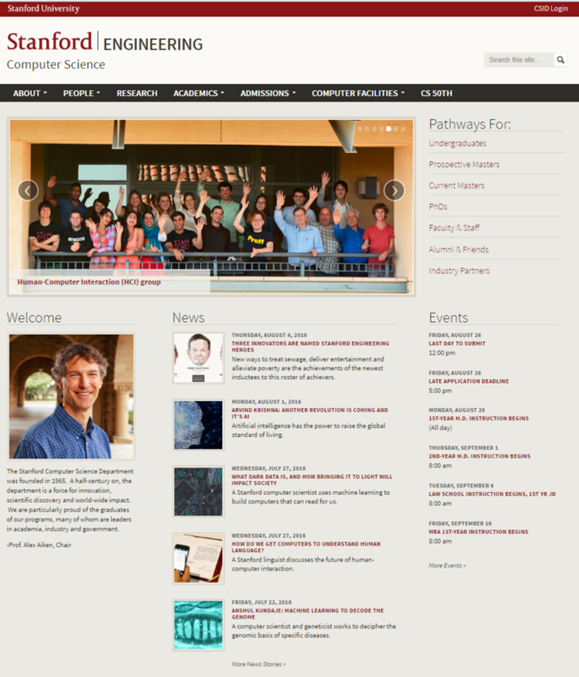
\includegraphics[scale=0.50]{imgs/chap_3/StanfordWebsite}} 
\subfloat[Box Structure]
{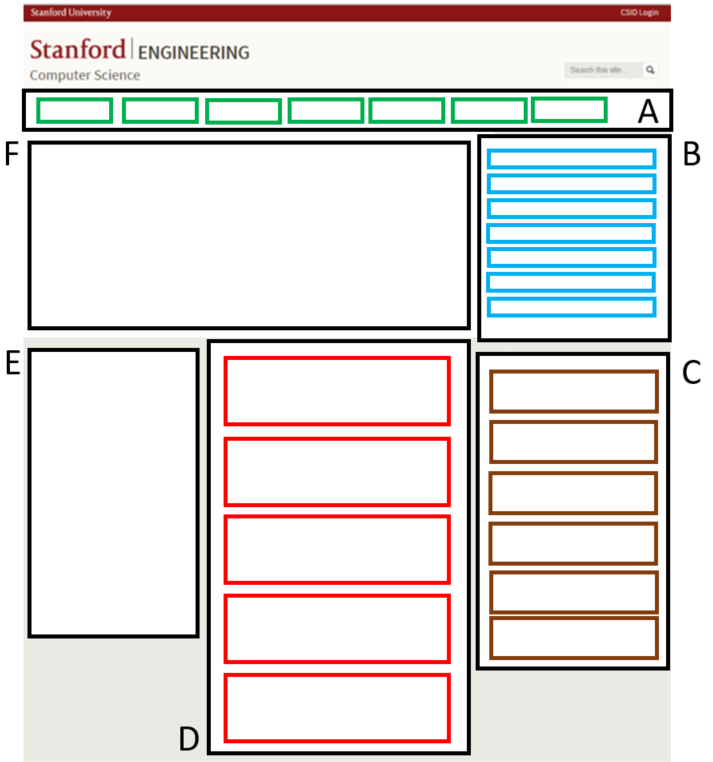
\includegraphics[scale=0.45]{imgs/chap_3/StanfordWebsiteBoxes}}\    
\subfloat[Structural Representation]
{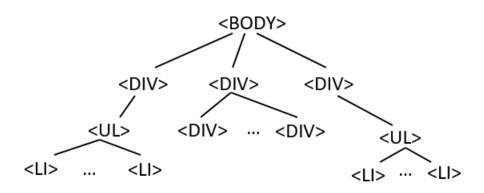
\includegraphics[scale=0.70]{imgs/chap_3/html}} 
\subfloat[Rendered Box Tree]
{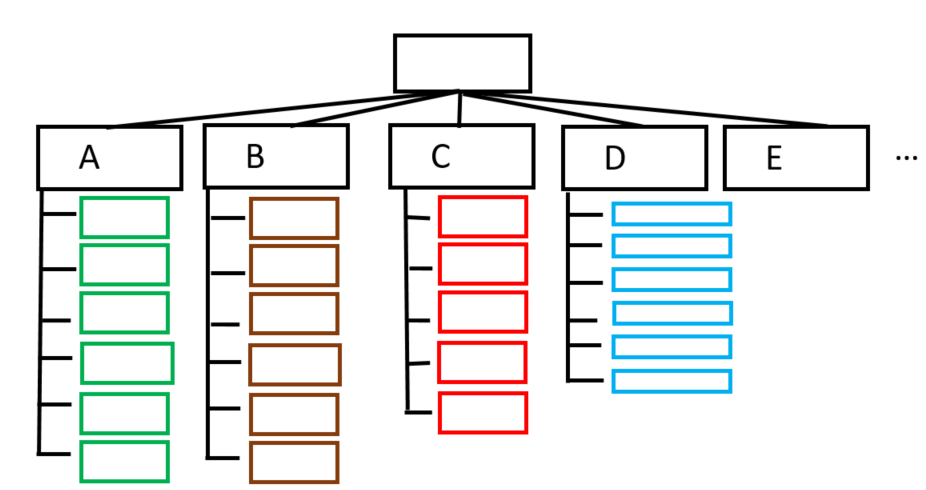
\includegraphics[scale=0.35]{imgs/chap_3/boxTree}}

\caption{}
\label{fig:Stanford}
\end{figure*}


Another important source of information proposed approach uses is the hyperlink structure of the website, which is formally introduced by the following definition:


\begin{definition}\label{def:website}A \textbf{Website} is a directed graph $G = (V, E)$, where $V$ is the set of web pages and $E$ is the set of hyperlinks. In most cases, the homepage $h$ of a website represents the website's entry page and, thus, allows the website to be viewed as a rooted directed graph. 
\end{definition}



As anticipated, the algorithm for the automatic identification of sitemaps exploits a sequential pattern mining step. The main  rationale behind this choice is to see a navigation path in a website as a sequence of urls and use sequences of urls to identify common (and frequent) navigation paths. Formally, a sequence is defined as follows:


\begin{definition}\label{def:sequence}\textbf{Sequence}:
Let $G = (V, E)$ be a website, a sequence $S$ is defined as $S=\langle t_1,t_2,\ldots,t_m \rangle$, where each item $t_j \in V$ denotes the web page at the $j$-th step in the navigation path $S$.
\end{definition}

A sequence $S=\langle t_1,t_2,\ldots,t_m \rangle$ is a \textbf{sub-sequence} of a sequence $S'=\langle a_1,a_2,\ldots,a_n \rangle$, if and only if integers $i_1, i_2, \dots, i_m$ exist, such that $1 \leq i_1 < i_2 < \dots < i_m \leq n$ and $t_1 = a_{i1}, t_2 = a_{i2}, \dots t_m = a_{im}$. We say that $S'$ is a \textbf{super-sequence} of $S$ or that $S'$ contains $S$.
\begin{example}
The sequence $S' = \langle a, b, d \rangle$ is a super-sequence of $S = \langle a,d \rangle $. On the contrary, $S'$ is not a super-sequence of $S'' = \langle e \rangle $, since the item $e$ is not equal to any item of $S'$.
\end{example}
Given a database of sequences $SDB$ and a single sequence $S$ the \emph{absolute support} of $S$ in $SDB$ is the number of sequences in $SDB$ which contain $S$, while its \emph{relative support} is the absolute support divided by the size of database (i.e., $|SDB|$).
With the term support I will refer to the relative support, unless otherwise specified:

\begin{equation}
\sigma(S) = \frac{|\{t \in SDB: S \textit{ is a  sub-sequence of } t\}|}{|SDB|}
\end{equation}

\noindent
A sequence is frequent if its support is greater than a user defined threshold. In our case the support defines the relationship strength among web pages.


Following the suggestion provided in \cite{Mobasher:2007}, we also exploit the definition of contiguous sequence which is formally defined as follows:

\begin{definition}\label{def:contiguousSeq}\textbf{Contiguous Sequence}: Given a sequence $S=\langle t_1,t_2,\ldots,t_m \rangle$ created from $G=(V,E)$, $S$ is contiguous if each item $t_i$ appears in $G$ contiguously to item $t_{i-1}$ (i.e. there is an edge between $t_{i-1}$ and $t_{i}$). 
\end{definition}


% Given a database of sequences $SDB$ and a single contiguous sequence $S$, the relative support of $S$ is defined as follows:
% \begin{equation}
% \sigma_{c}(S) = \frac{|\{t \in SDB: S \textit{ is a contiguous subsequence of } t\}|}{|SDB|}
% \end{equation}

The task of sequential pattern mining indicates the task of discovering frequent (sub-)sequences (contiguous sequences) from $SDB$. This is considered computationally challenging because  algorithms have to generate and/or test a combinatorially explosive number of intermediate sub-sequences. For this reason, we consider the simpler problem (in terms of time complexity) of identifying \textit{closed} sequential patterns which are compact and provide a lossless representation of all sequential patterns. A closed sequential pattern (or, simply, a closed sequence) is defined as follows:

\begin{definition}\label{def:closedSeq}\textbf{Closed Sequence}: %Given two sequences (contiguous sequences) $S_i$ and $S_j$, if $S_i$ is a supersequence of $S_j$ and their support in $SDB$ is the same, we say that $S_i$ absorbs $S_j$. 
A sequential pattern (contiguous sequential pattern) $S_j$ is \textbf{closed} if and only if it is frequent and its support is different from all of its frequent super-sequences.
\end{definition}
\begin{example}
Figure \ref{fig:myfigs}(b) shows an example of a database of sequences. Sequence $\langle h \rangle$ is closed because no super-sequences of $\langle h \rangle$  with the same support exist. 
On the contrary, the sequence $\langle h, d \rangle$ is not closed because the super-sequence $\langle h, b, d \rangle$ has the same support of $\langle h, d \rangle$.
\end{example}
\noindent



The last definition we have to provide before discussing technical details of the method is that of sitemap. This definition is particularly important since it defines the goal of the proposed method.



\begin{definition}\label{def:sitemap}\textbf{Sitemap}:
Given a web graph $G = (V,E)$ where $h\in V$ is the homepage, a user-defined threshold $t$ and a weight function $w:~E~\rightarrow~\mathbb{R} $, then $T = \argmax_{{T_i}}{\Phi(T_i)}$ is a sitemap if:
\begin{enumerate}
\item $T_i= (V_i',E_i')$ is a tree rooted in $h$, where $V_i' \subseteq V$ and $E_i' \subseteq E$;
\item $ \Phi(T_i) = \sum_{e \in E_i'} w(e)$;
\item  $\forall~e = (j_1,j_2) \in E_i', j_2 \in webList(j_1)$, that is, the url of the web page $j_2$ is contained in some \textit{web list} of the web page $j_1$ (See Def. \ref{def_chap2:list}); 
\item $\forall e \in E_i',~w(e) \geq t$. 
\end{enumerate} 
\end{definition}


\noindent

What remains unspecified in this (general) definition is the meaning of $w(\cdot)$ and the way the tree $T$ is generated. These aspects are discussed in the following section where we describe the method and instantiate aspects intentionally kept as parameters in Definition \ref{def:sitemap}.
We only anticipate that our solution does not need to enumerate all possible trees $T_i \subseteq G$ to optimize $\Phi(\cdot)$, yet it is able to extract directly $T$ analyzing a sub-graph of the website.

\section{Methodology}
\label{sec:methodology}


The problem we consider is that extracting the website's sitemap, defined according to Definition \ref{def:sitemap}. To achieve this goal, I combine different techniques which have roots in  web and data mining research areas: \emph{i)} Information extraction for identifying potential navigation systems in web pages in form of web-lists; \emph{ii) } Random Walk theory to extract navigation paths; \emph{iii)} Sequential pattern mining for finding the most frequent paths which describe the hierarchical structure of the website. 


In the first step of the proposed methodology we perform website crawling. Crawling uses web pages' structural and visual information to extract web lists in order to mitigate problems coming from noisy links. 
The output of this phase is the website graph $G$, where each node represents a single page and edges represent hyperlinks. Details of this step are described in Section~\ref{3Crawling}.
In the second phase we generate sequences of urls (i.e., web pages), which describe navigation paths. This is done by exploiting random walks extracted from the crawled website's graph. In the third phase we mine closed frequent sequences of urls (i.e., closed frequent navigation paths) in form of a tree.
In the last step the tree of closed sequences is analyzed in order to extract the sitemap. This step requires the transformation of the tree of sequences in a tree of web pages such that the obtained tree has the homepage as root and a web page appears only once, that is, it is not possible to have multiple paths that connect the homepage with a web page. 

% Finally, in the last phase is applied a pruning step to filter, for each node $v \in V'$, the best path which connect the homepage to $v$. The extracted tree is the website sitemap.


\subsection{Sequence Database Generation}
\label{dbGeneration}

To capture and codify correlations among graph's nodes (i.e. web pages) I use the Random Walk with Restart from Homepage (RWRH) approach. It can be considered a 
particular case of Random Walk with Restart, obtained setting a single node (i.e. the homepage) as starting vertex. Random walk with restart is widely adopted in several works to infer structural properties of nodes in a graph through the analysis of the global structure of the whole network.

Using this approach, web pages closer to the homepage have higher probability to be reached than those at deeper levels. %Moreover, the random walker with restart assigns higher probabilities to web pages closer to the homepage than those at deeper levels. 
This is coherent with the organization typically followed in the website navigation where navigation systems closer to the homepage belong to shallower levels of the website hierarchy.

Therefore, given the web graph $G$ extracted in the previous step, and two number $rwrLength, dbLength \in  \mathbb{N} $, the random walk theory is used to navigate the web graph $G$ from the homepage $h$. 
The output of this phase is a sequence database $SDB$ composed by $dbLength$ random walks having length $rwrLength$ and starting from $h$. As defined in \cite{Pons:2006}, increasing the length $rwrLength$ of a random walk starting at node $i$, the probability to reach a node $j$ tends to depend on the degree of $j$. As suggested in \cite{Pons:2006} we generate short random walks in the way that the random walker tends to get "trapped" into densely connected parts of the graph corresponding to communities (i.e. sibling pages in the sitemap) and for avoiding to infer false correlations among web pages due the nodes' degree.
Algorithm~\ref{3alg:datasetGeneration} describes the generation process of the sequence dataset.
Figure~\ref{fig:SDB} shows a sequence database obtained from the web graph in Figure~\ref{fig:graph}


\begin{algorithm}[tb]
\caption{rwrGeneration(rwrLength, dbLength, G, $\alpha$)}
\label{3alg:datasetGeneration}
\begin{algorithmic}[1]
\renewcommand{\algorithmicrequire}{\textbf{Input:}}
\newcommand{\RETURN}[1]{\textbf{return} #1}
\renewcommand{\algorithmicensure}{\textbf{Output:}}
\renewcommand{\algorithmiccomment}[1]{$//$ \textit{#1}}
\renewcommand{\algorithmicforall}{\textbf{for each}}
\newcommand{\getRandomVertex}[1]{ \textit{getRandomVertex}(#1); }
\newcommand{\getNextRandomVertex}[1]{ \textit{getRandomOutlink}(#1); }
\newcommand{\add}[1]{ \textit{add}(#1); }

\REQUIRE int rwrLength, int dbLength, Graph G, float $\alpha$;
\ENSURE List$<$List$<$URL$>>$ randomWalks;
	\FORALL{i $\in$ Range(0, dbLength)}
	    \STATE w = List()
	    \STATE w[0] = G.homepage
		\FORALL{j $\in$ Range(1, rwrLength) }
		\STATE $\lambda$ = Math.random()
		\IF{$\lambda > \alpha$}
		\STATE w[j] = G.\getNextRandomVertex{w[j-1]}
		\ELSE 
		\STATE w[j] = w[0]
		\ENDIF
		\ENDFOR
		\STATE randomWalks.\add{w}
 	\ENDFOR
\RETURN randomWalks

\end{algorithmic}
\end{algorithm}
  
%For this reason, we generate short random walks, in the way that the random walker tends to get “trapped” into densely connected parts of the graph corresponding to communities and to avoid the effect predicted in \cite{Pons:2006}.
%it is be too influenced by nodes degree .

\subsection{Closed sequential patter mining}
Given the sequence database (SDB), extracted in the Section~\ref{dbGeneration}, and a user defined threshold $t$ (i.e. minimum support), we apply a closed sequential pattern mining algorithm to extract all the frequent sequences. In this phase we used the algorithm CloFAST~\cite{Fumarola:2015} as closed sequential pattern mining algorithm. It  showed to provide compact results, saving computational time and space if compared with other closed sequential pattern mining algorithms.
CloFast returns a tree $T_{CloFAST} = (V', E')$ and a weight function $\sigma : E' \rightarrow \mathbb{R} $ which associates each edge $e=(j_1,j_2)\in E'$  with the \textit{relative} support of the sequence $\langle h, \ldots, j_1,j_2\rangle$ in $T_{CloFAST}$.

Figure~\ref{3fig:tree1} shows an example of tree extracted by CloFAST for the input sequence dataset in figure~\ref{3fig:sf1}. 

\begin{figure*}
\center
\subfloat[]{
\label{3fig:tree1}
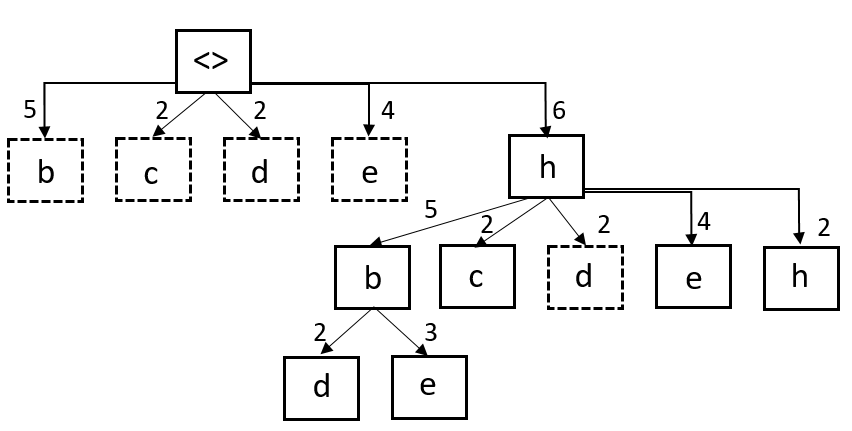
\includegraphics[scale=0.45]{imgs/chap_3/clofast}} \
\subfloat[]{
\label{3fig:tree2}
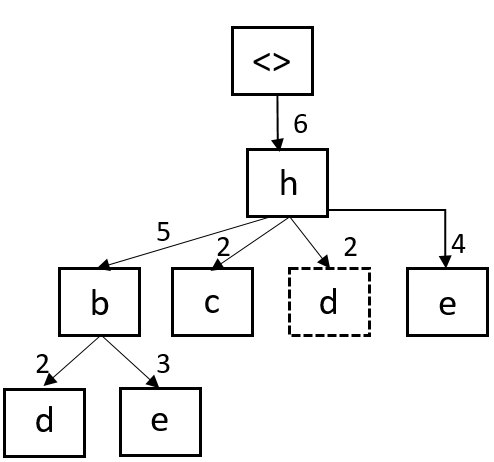
\includegraphics[scale=0.45]{imgs/chap_3/clofastPruned}}
\subfloat[]{
\label{3fig:tree3}
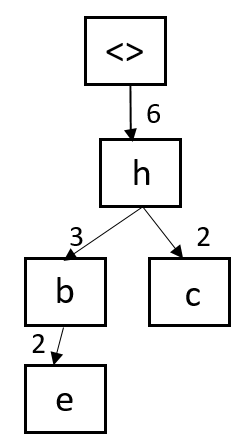
\includegraphics[scale=0.45]{imgs/chap_3/clofastContiguous}}
\caption{(a) Frequent sequence tree extracted by CloFAST with absolute minsup = 3 and SDB in fig. \ref{fig:myfigs}(b). Nodes with
dashed borders represent non-closed nodes; (b) Frequent sequences tree extracted by extended version of CloFAST and having the support as weight function; (c) Contiguous sequences tree extracted by extended version of CloFAST and having the contiguous support as weight function.}
\label{3fig:clofast}
\end{figure*}

Since a contribution of this chapter is to compare the sitemaps extracted considering two different types of sequences (i.e. sequential patterns and contiguous sequential pattern), I extend CloFAST by allowing it to also extract contiuous sequential patterns. 

To extract the weighted tree of contiguous sequences from $T_{CloFAST}$ I benefit of the data structure, called \textit{Vertical id-List} (VIL) provided by CloFAST for support counting purpose and for extracting frequent sequences. In the following we give a brief definition of a VIL:
\begin{definition}[Vertical Id-list]
Let $SDB$ be a sequence database of size \emph{n} (i.e. $|SDB| = n$), $S_j \in SDB$ its j-th sequence ($j \in \{1,2,\ldots,n\}$), and $\alpha$ a sequence associated to a node of the tree, its \emph{vertical id-list}, denoted as $VIL_{\alpha}$, is a vector of size $n$, such that for each $j=1,\ldots,n$
\begin{displaymath}
VIL_\alpha[j] = \left\{ \begin{array}{ll}
\textrm{$[pos_{\alpha,1}, pos_{\alpha,2}, \ldots, pos_{\alpha,m}]$ }\ \ \ \ & \textrm{if $S_j$ contains $\alpha$}\\
null & \textrm{otherwise}
\end{array} \right.
\end{displaymath}
where \emph{$pos_{\alpha,i}$} is the end position of the $i$-th occurrence ($i\leq m$) of $\alpha$ in $S_j$. 
\end{definition}

\begin{example}
\label{ex:vil}
Figure \ref{3fig:VILhb} shows the $VIL$ of the sequence $\alpha = \langle h , b \rangle$. Values in $VIL_{\alpha}$ represent the end position of the occurrences of the sequence $\alpha$ in the sequences of Figure \ref{fig:SDB}. In particular, the first element (list with only value 2) represents the position of the first occurrence of web page $b$, after the web page $h$ (i.e. $b$ is the last item in $\alpha$), in the first sequence $S_1$. The second element is (list with values 2 and 4) the position of the first item $b$ (after $a$) in the sequence $S_2$.
The other values are respectively list with only value 3 (for sequences $S_3$), list with only value  2 (for $S_4$) \emph{null} (for $S_5$) and list with only value 3 (for $S_6$).  In particular, the fifth element is null since $\alpha$ is not present in $S_5$.
Finally, the support of $\alpha$ is the number of not null elements in $VIL_{\alpha}$, that is 0.71.
\end{example}
\begin{figure}[tb]
  \centering
  \subfloat[]{\label{3fig:sf0}
  	\centering
    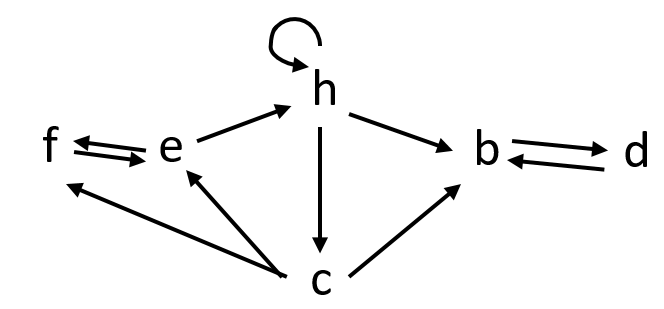
\includegraphics[scale=0.40]{imgs/chap_3/graph}
    \label{fig:graph}}
  \centering
  \subfloat[]{\label{3fig:sf1}
  	\centering
    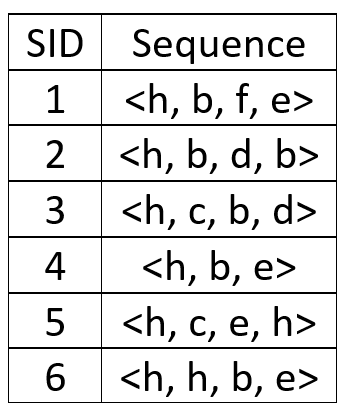
\includegraphics[scale=0.40]{imgs/chap_3/sequences.png}
    \label{fig:SDB}}
  \subfloat[]{\label{3fig:sf2}
  	\centering
  	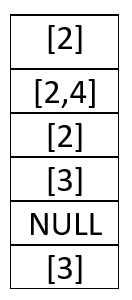
\includegraphics[scale=0.40]{imgs/chap_3/VILhb.png}
    \label{3fig:VILhb}}
  \caption{(a) Web Graph rooted at h; (b) Sequence Database (SDB), that is, a set of tuples (SID, Sequence), where SID is a sequence-id and Sequence is a random walk with restart from the homepage; (c) VIL for the sequence $\alpha = \langle h,b \rangle$.}
  \label{fig:myfigs}
\end{figure}
We modify the CloFAST implementation creating two pruning method that: \emph{i)} stop the generation of frequent sequences which start from a node different from the homepage; \emph{ii)} extract contiguous sequences. In particular, starting from the root of $T_{CloFAST}$, the function \textit{contiguous($\cdot$)} (see Algorithm~\ref{alg:contiguos}) is iteratively applied to update the node's VILs. It looks for possible holes in the sequences by botton-up clibing the sequence tree $T_{CloFAST}$. An hole is found when the condition at line 10 is not satisfied. Returned VIL of a node $n$ is used to calculate its contiguous support without scanning the sequence database SDB:
$\sigma_c(n) = \{j|vil = contiguous(n, T_{CloFAST}) \wedge  vil[j][1]= h\}$.
Therefore, if the contiguous support of $n$, $\sigma_c(n)$, is greater of the threshold $t$, the function is applied to its children, otherwise the node is pruned. We call the returned tree $T'_{CloFAST}$

\subsection{Sequence Pruning}
The trees $T_{CloFAST}$ (for sequential patterns) and $T'_{CloFAST}$ (for contiguous sequential patterns), extracted in the previous step, may contain multiple frequent paths to reach, from the homepage, a given node (web page). For example, in Figure~\ref{3fig:tree2} the web page $e$ can be reached using the frequent patterns $h\rightarrow b \rightarrow e$ and $h\rightarrow e$.
Since in the sitemap each web page can be reached by only one path starting from the homepage, the last task of the sitemap generation is the pruning process. Therefore, the goal of this step is to select for each web page included in the frequent sequence (contiguous sequence) tree, the best path to reach it.

A sequence  $\alpha = \langle u_1, \dots, u_i, u_{i+1}, \dots, u_n \rangle \in T_{CloFAST}$ is pruned if:
\begin{enumerate}
%\item $u_1 \neq h$, with $h$ the website's homepage;
\item $\nexists~(u_i, u_{i+1}) \in E$, with $1 \leq i < n$ and $u_1 = h$;
\item $\exists \beta = \langle h, \dots, u_n \rangle \in T_{CloFAST}$ ($T'_{CloFAST}$) and $\beta \neq \alpha$ such that 
\begin{equation}
\label{eq:pruning}
\sum_{e' \in T_{\beta}}w(e') + w(\beta) > \sum_{e \in T_{\alpha}}w(e) + w(\alpha)
\end{equation}
\end{enumerate}
%The first constraint prunes all frequent sequences which start from a node different from the homepage.
The first constraint ensures that frequent paths that do not exist in the crawled graph G are removed (see Def.~\ref{def:sitemap}.3).  The second constraint allows us to select for each node in $V'$ which can be reached by multiple frequent sequences, starting from the homepage, the best path. 
 In particular, for each node $u_n$, ending node of multiple frequent sequences (e.g. $\alpha$ and $\beta$), we compare all the sub-trees of $T_{CloFAST}$ ($T'_{CloFAST}$) having $u_n$ as root (e.g. $T_\alpha$ and $T_\beta$). From them, we only keep that one which maximize the sum of its edges plus the weight of the path starting from \emph{h} and reaching $u_n$ (e.g. $w(\alpha)$ and $w(\beta)$). For the case of sitemap extraction using sequential patterns we associate to the weight function $w(\cdot)$, defined in Def.~\ref{def:sitemap}, the support function $\sigma(\cdot)$ returned by CloFAST. For the case of sitemap extraction using contiguous sequential patterns we associate to $w(\cdot)$ the contiguous support function $\sigma_c(\cdot)$ calculated by Algorithm~\ref{alg:contiguos}. 

\begin{algorithm}[tb]
\begin{algorithmic}[1]
\renewcommand{\algorithmicrequire}{\textbf{Input:}}
\renewcommand{\algorithmicensure}{\textbf{Output:}}
\newcommand{\RETURN}[1]{\textbf{return} #1}
\renewcommand{\algorithmiccomment}[1]{$//$ \textit{#1}}
\newcommand{\getPos}[1]{ \textit{getPos}(#1); }
\newcommand{\length}[1]{ \textit{length}(#1); }
\newcommand{\shift}[1]{ \textit{next}(#1); }
\newcommand{\getVil}[1]{ \textit{getVil}(#1); }
\newcommand{\getParent}[1]{ \textit{getParent}(#1); }
\REQUIRE $T$: a sequence tree extracted by CloFAST; n: node of $T$
\ENSURE vil: the VIL of the sequence at node n such that the contiguous condition is satisfied.

\STATE vil = \getVil{n}
\STATE parent = \getParent{n}
\REPEAT 

	\STATE parentVil = \getVil{parent}
	\FORALL{ $j = 1 \ldots$\length{vil}}
		\STATE i=0; 	contiguous =  $FALSE$;
		\REPEAT
				\STATE z=0;
				\REPEAT
				\IF{ vil[j][i] = parentVil[j][z]+1 }
					\STATE vil[j] = parentVil[j][z..(len(parentVil[j])-1)];
					\STATE contiguous = $TRUE$ ;
				\ENDIF
			\UNTIL{$++z \leq i $ AND !contiguous}
			\IF{!contiguous}
				\STATE vil[j] = $NULL$\;				
			\ENDIF
		\UNTIL{$++i < len(vil[j])$ AND !contiguous }
	\ENDFOR
\STATE n = parent
\STATE parent = \getParent{n}\;
\UNTIL{parent != root(T)}
\RETURN vil;
\caption{contiguous(T,n)}
\label{alg:contiguos}
\end{algorithmic}
\end{algorithm}




\section{Experiments and Discussion}
\label{sec:experiments}
The aim of this chapter is to answer to the following research questions: 1) Which is the real contribution of combining the random walk teory with structured data with respect to use the content and the whole hyperlink structure? 2) Which is the real contribution of extracting hierarchies based on  sequential patterns with respect to extract hierarchies based on $contiguous$ sequential patterns. 
For this reason we compare the performances of SMAP (i.e. sitemap generation through sequential patterns) and $SMAP_{sc}$ (i.e. sitemap generation through $contiguous$ sequential patterns) with a state-of-art algorithm, that is HTDM~\cite{Weninger:2012}.

The empirical evaluation of these algorithms was not a trivial task because, at the best of our knowledge, there is no dataset generated for the specific task of sitemap extraction. 
Thus, two solutions were possible: \emph{i)} involving human experts to extract the hierarchical organization of websites and generating a ground truth dataset for each considered website; \emph{ii)} using existing sitemap pages, which are manually generated by web masters and provided by some website, as ground truth. 


In the first case, the involvement of experts requires extensive human effort and working time. This is not feasible in the context of the Web especially for websites having a great amount of web pages strongly connected and websites having deep hierarchies. In the second case, sitemap pages are in general manually created by web designers. Therefore, the risk is that sitemap pages are not updated (i.e. they can contain links to non-existent pages or they ignore the existence of new sections) or are very abstract (i.e. contain shallow hierarchies composed by few pages). For this reason, to empirically evaluate SMAP, I have performed experiments on following websites which provide updated sitemap pages: \emph{cs.illinois.edu}, \emph{www.cs.ox.ac.uk}, \emph{www.cs.princeton.edu}, and \emph{www.enel.it}. 

The evaluation has been performed in terms of Precision, Recall and F-measure of edges. In particular, the Precision measures how many of the extracted edges belong to the real sitemap. The Recall measures how many edges, belonging to the real sitemap are extracted.
%the discovered edges are true positive elements of the real sitemap.
I also included the F-Measure which is the weighted harmonic means of Precision and Recall. These measures are evaluated counting how many edges of the real sitemap are found by the algorithm under analysis (i.e. SMAP, $SMAP_{cs}$, HDTM).
More formally:


\begin{equation}
Precision= \frac{|\{e| e\in SMAP(G) \wedge e\in GT\_Sitemap \}| }{|\{e| e\in SMAP(G) \}| }
\end{equation} 

\begin{equation}
Recall=\frac{|\{e| e\in SMAP(G) \wedge e\in GT\_Sitemap \}| }{|\{e| e\in GT\_Sitemap \}| }
\end{equation} 


\begin{equation}
F = \frac{2(precision \times recall)}{precision + recall}
\end{equation} 

\noindent In these formulas $SMAP(G)$ represents the set of edges extracted by $SMAP$, whereas $GT\_Sitemap$ represents the set of edges in the real sitemap (ground truth).



%We analyzed the effectiveness of proposed approach (SMAP) with four real websites: \textit{cs.illinois.edu, www.cs.ox.ac.uk, www.cs.princeton.edu}, and \textit{www.enel.it}.  Each analyzed website contains a sitemap provided by the website's organization which allows us to have a ground truth and evaluate the extracted sitemaps in terms of precision, recall and F-measure of edges.
%The results are compared with those obtained by HDTM~\cite{Weninger:2012}. For HDTM  we set $\gamma = 0.25$ (to avoid too shallow or too deep hierarchies) and $5,000$ Gibbs iterations, as suggested by the authors in their paper. 
Table \ref{tableResSitemap} presents the main results. For HDTM  I set $\gamma = 0.25$ (to avoid too shallow or too deep hierarchies) and $5,000$ Gibbs iterations, as suggested by the authors in their paper. For SMAP and $SMAP_{cs}$ I set $rwrLength =10 $ and $dbLength=500.000$ (See Section \ref{dbGeneration}). Moreover, I analyze the effectiveness of SMAP and $SMAP_{cs}$ varying the minimum support. It is interesting to note that when the minimum support threshold decreases, we are able to obtain deeper and wider sitemaps. While, as expected, by reducing the minimum support threshold, precision increases and recall decreases. 
This is due to the fact that, by decreasing the support, the number of generated sequences increases and the extracted hierarchy becomes deeper and wider, including website sections which are not included in the sitemap page. This behaviour can be observed by analyzing the F-measure which, from website to website, shows different trends for different values of minimum support.

Interestingly, both versions of our algorithm significantly outperform HDTM, independently of the website and of the minimum support threshold. 
This can be motivated by the different nature of the two algorithms: on the contrary of our approach, HDTM organizes website's pages in a hierarchy using the distribution of web pages' terms. Then, it can happen that, for example, for a Computer Science department website HDTM organizes the web page of a \emph{professor} as a child of its \emph{research area} web page rather than as a child of the \emph{professors} web page. In this way, web pages clustered together as siblings in the hierarchy by web masters are split in different parts of the extracted hierarchy.

Finally comparing the sitemaps extracted using sequential patterns and $contiguous$ sequential patterns we can observe that in general SMAP outperforms $SMAP_{sc}$. This is due by the fact that $SMAP_{sc}$ extracts narrower and shallower hierarchies compared with $SMAP$. In fact, setting low support thresholds $SMAP_{sc}$ obtain better results than SMAP in terms of Recall but, since it is unable to extract the deepest levels, it obtains lower results in terms of Precision.

%What is interesting is that F-measure depends on the website and, more precisely, on the level of details of the ground truth (real sitemaps). 

\begin{table}[t]

\centering

\begin{tabular}{|c|c|c|c|c|c|}
\hline
Website & Algorithm & min. supp. & Precision & Recall & F-Measure  \\
\hline
cs.illinois.edu & SMAP & 0.005  & 0.38 & \textbf{0.78} & 0.51 \\
cs.illinois.edu & $SMAP_{cs}$ & 0.005  &0.1	& 0.65	& 0.17 \\
cs.illinois.edu & SMAP & 0.001  & 0.66 & 0.48 & \textbf{0.56} \\
cs.illinois.edu & $SMAP_{cs}$ & 0.001  & 0.35& 0.76 & 0.48  \\
cs.illinois.edu & SMAP & 0.0005 & 0.66 & 0.33 & 0.44 \\
cs.illinois.edu & $SMAP_{cs}$ & 0.0005  & 0.35 & 0.33  & 0.34  \\
cs.illinois.edu & SMAP & 0.0001 & \textbf{0.75} & 0.26  & 0.38 \\
cs.illinois.edu & $SMAP_{cs}$ & 0.0001  & 0.61 & 0.35  & 0.45  \\
cs.illinois.edu & HDTM & $-$ &  0.12 & 0.1 & 0.11 \\
\hline
cs.ox.ac.uk &  SMAP & 0.005  & \textbf{0.72} & 0.3 & \textbf{0.42} \\
cs.ox.ac.uk &  $SMAP_{cs}$ & 0.005  & 0.27 & \textbf{0.41} & 0.33 \\
cs.ox.ac.uk &  SMAP & 0.001 & \textbf{0.72} & 0.21 & 0.33 \\
cs.ox.ac.uk &  $SMAP_{cs}$ & 0.001  & 0.60& 0.18 &1.28  \\
cs.ox.ac.uk &  SMAP & 0.0005  & 0.72 & 0.21 & 0.33 \\
cs.ox.ac.uk &  $SMAP_{cs}$ & 0.0005  & 0.60& 0.17 &0.27  \\
cs.ox.ac.uk &  SMAP & 0.0001  & \textbf{0.72} & 0.21 & 0.33 \\
cs.ox.ac.uk &  $SMAP_{cs}$ & 0.0001  & 0.60& 0.17 &0.27  \\
cs.ox.ac.uk &  HDTM & $-$ & 0.37 & 0.15 & 0.21 \\
\hline
cs.princeton.edu &  SMAP & 0.005  & 0.61 & \textbf{0.55} & \textbf{0.58} \\
cs.princeton.edu &  $SMAP_{cs}$ & 0.005  & 0.1& 0.22 & 0.14 \\
cs.princeton.edu &  SMAP & 0.001  & 0.89 & 0.23 & 0.36 \\
cs.princeton.edu &  $SMAP_{cs}$ & 0.001  & 0.6&  0.55& 0.58 \\
cs.princeton.edu &  SMAP & 0.0005  & 0.89 & 0.2 & 0.33 \\
cs.princeton.edu &  $SMAP_{cs}$ & 0.0005  & 0.6 &0.32  &0.41  \\
cs.princeton.edu &  SMAP & 0.0001 & \textbf{0.9}1 & 0.13 & 0.23 \\
cs.princeton.edu &  $SMAP_{cs}$ & 0.0001  & 0.73 & 0.18 & 0.29  \\
cs.princeton.edu &  HDTM & $-$ & 0.36 & 0.08 & 0.13 \\
\hline
enel.it & SMAP & 0.005 & 0.31 & 0.74 & 0.43 \\
enel.it &  $SMAP_{cs}$ & 0.005  &0.1 & 0.47 & 0.16  \\
enel.it & SMAP & 0.001  & 0.36 & 0.72 & 0.48 \\
enel.it &  $SMAP_{cs}$ & 0.001  & 0.31& 0.73 & 0.43 \\
enel.it & SMAP & 0.0005  & 0.8 & 0.73 & 0.76 \\
enel.it &  $SMAP_{cs}$ & 0.0005  & 0.31 & 0.73  & 0.43  \\
enel.it & SMAP & 0.0001  & \textbf{0.8} & 0.73 & 0.76 \\
enel.it &  $SMAP_{cs}$ & 0.0001  & 0.77 & \textbf{0.8}  & \textbf{0.79}  \\
enel.it & HDTM & $-$ & 0.35 & 0.75 & 0.48 \\
\hline
\end{tabular}
\caption{Experimental results of SMAP, $SMAP_{cs}$ and HDTM.}
\label{tableResSitemap}
\end{table}
%vedi questo link per intro su navigation system e search
%\url{https://books.google.it/books?hl=it&lr=&id=mDI72_9-bw0C&oi=fnd&pg=PR14&ots=yVrdtw7tEv&sig=TzAHTw_xuAJeBn75iuFZxNOLtvU#v=onepage&q&f=false}

\chapter{CloFAST: Closed Sequential Pattern Mining using Sparse and Vertical Id-Lists}
\input{chap_5/CloFAST}


\chapter{Conclusion}

The World Wide Web, in its current form, is modern legacy system where data cannot be automatically accessed and manipulated. Goal of Web Mining is therefore to discover and to extract valuable information in the way to improve and automate the information gathering process. 

In this thesis I face the problem of mining structured data encoded in web pages or hidden in the topological structure of a website. 
 This is due analyzing the most important representations of a web page (i.e. textual, visual, structural representation) and combining the extracted intra-page information with inter-page information (i.e. hyperlink structure).  
In particular this thesis focus on two main open challenges, that is combining structured data splitted on multiple web pages and organizing web pages semantically similar.

In the first case,  similar to databases, where a view can represent a subset of the data contained in a table, websites split a logical list in multiple views in order to avoid information overload and to facilitate users' navigation. However, the data stored in such \emph{logical list} need to be automatically extracted to enable building services for market intelligence, synonyms discovery, question answering and data mashup. The approach presented in this thesis solves this open issue.
Experimental results show that the algorithm is extremely accurate and it is able to extract \textit{logical lists} in a wide range of domains and websites with high precision and recall.
Part of this future work will involve tasks such as indexing the Web based on lists and tables, answering queries from lists, and entity discovery and disambiguation using lists.

In the second case, web pages can be grouped based on different types of features. To solve this open issue, I present two unsupervised and domain-independent approaches. In particular, the first method combines information about content, web page structure and hyperlink structure in a single vector space representation which can be used by any traditional and best-performing clustering algorithms. To take into account the hyperlink structure I exploit recent advances in natural language processing by adapting the skip-gram model. %In the evaluation I have analyzed two research questions: 1) Which is the real contribution of  combining  content  and  hyperlink  structure  in  a  single vector space representation with respect to using only either textual content or hyperlink structure? 2) Which is the real contribution  of  exploiting  web  pages  structure  (i.e.  HTML formatting)  and,  specifically,  the  role  of  using  web  lists  to reduce noise and improve clustering results? 
Experiments results show that content and hyperlink structure of web pages provide  different  and  complementary  information which can improve the efficacy of clustering algorithms. Moreover, experiments do not show statistical differences between results which use web lists and results obtained ignoring web page structure. 
The second approach proposed in this thesis is related with the automatic sitemap generation. A sitemap represents an explicit specification of the design concept and knowledge organization of a website. Intuitively, sibling Web pages this hierarchy should be of the same type (e.g. professors web pages, courses web pages, etc.), and parents and children pages should be of more general and more specific types respectively. For this purpose I propose a new method which automatically discovers the hierarchical organization of a website by using the content and the hyperlinks structure of web pages. Experimental results prove that the proposed approach outperforms HDTM, a state-of-art algorithm which extract the hierarchical structure of a website through the analysis of contents and hyperlinks 




\bibliographystyle{alpha} %mettere plain o alpha
\bibliography{bibliography}

% ----------------- Insert index
%\addcontentsline{toc}{chapter}{Index of terms}
%\printindex
%\input{tesi.ind}
\clearpage
\vspace*{6cm}

% ----------------------------------------------------------------
\end{document}
% ----------------------------------------------------------------
